\documentclass[a4paper,12pt]{report}

\usepackage{geometry}
\geometry{a4paper,left=18mm,right=18mm, top=3cm, bottom=2cm}

\usepackage{lmodern}
\usepackage[T1]{fontenc}
\usepackage{eurosym}
\usepackage{setspace}
\usepackage[latin1]{inputenc}
\usepackage{graphicx}
\usepackage[ngerman]{babel}
\usepackage[solution_on]{mathematik} % solution_on/off
\usepackage{blindtext}
\setcounter{Zufall}{0}


\pagestyle{empty} %PAGESTYLE: empty, plain, fancy
\onehalfspacing %Zeilenabstand
\setcounter{secnumdepth}{-1} % keine Nummerierung der �berschriften



%
%
%%%%%%%%%%%%%%%%%%%%%%%%%%%%%%%%%%%%%%%%%%%%%%%%%%%%%%%%%%%%%%%%%%%%%%%%%%%%%%%%%%%%%%%%%% DOKUMENT - ANFANG %%%%%%%%%%%%%%%%%%%%%%%%%%%%%%%%%%%%%%%%%%%%%%%%%%%%%%%%%%%%%%%%%%%%%%%%%%%%%%%%%%%%%%%
%
%
\begin{document}
\section{K1 - DZ.ef - 2 - Stellenwerte - OA - QueUnb}

\begin{beispiel}{0} %PUNKTE DES BEISPIELS
				Schreibe die Zahl mit Hilfe von Stellenwerten auf!\leer
					
					$40,003047=$ \antwort{4Z\,3t\,4ht\,7m}
\end{beispiel}%
\hrule  \leer

\section{K1 - DZ.ef - 3 - Runden auf Hundertstel - OA - QueUnb}

\begin{beispiel}{0} %PUNKTE DES BEISPIELS
				Runde die Dezimalzahl auf Hundertstel!\leer
					
					$3,4089\approx$ \antwort{3,41}
\end{beispiel}%
\hrule  \leer

\section{5 - MAT - WS 2.2, WS 3.1, WS 3.3 - Mathematikschularbeiten - BIFIE Aufgabensammlung}

\begin{langesbeispiel} \item[0] %PUNKTE DES BEISPIELS
Wenn in der Oberstufe in einem Semester höchstens zwei Mathematikschularbeiten vorgesehen sind, muss jede versäumte Schularbeit nachgeholt werden.
				Ein Mathematiklehrer hat auf Basis seiner langjährigen Erfahrung die untenstehende Tabelle erstellt. Dabei beschreibt $h(n)$ die relative Häufigkeit, dass bei einer Schularbeit insgesamt $n$ Schüler/innen fehlen.\vspace{0,3cm}
				
\begin{center}
				\begin{tabular}{|c|c|c|c|c|c|c|c|c|c|} \hline
				$n$&0&1&2&3&4&5&6&7&>7\\ \hline
				$h(n)$&0,15&0,15&0,2&0,3&0,1&0,05&0,03&0,02&0\\ \hline
				\end{tabular}	
\end{center}%Aufgabentext

\begin{aufgabenstellung}
\item %Aufgabentext

\Subitem{Gib an, mit wie vielen Fehlenden der Mathematiklehrer im Durchschnitt bei jeder Schularbeit rechnen muss.} %Unterpunkt1
\Subitem{Lässt sich aus dem errechneten Durchschnittswert mit Sicherheit behaupten, dass bei jeder Mathematikschularbeit mindestens eine Schülerin/ein Schüler fehlt? Begründe deine Antwort.} %Unterpunkt2

\item %Aufgabentext

\Subitem{Kreuze die beiden zutreffenden Aussagen an!
	
	\multiplechoice[5]{  %Anzahl der Antwortmoeglichkeiten, Standard: 5
					L1={Es kann nie passieren, dass acht Schüler/innen bei einer Schularbeit fehlen.},   %1. Antwortmoeglichkeit 
					L2={Die Wahrscheinlichkeit, dass bei einer Mathematikschularbeit niemand fehlt, ist gleich groß wie die Wahrscheinlichkeit, dass eine Schülerin/ein Schüler fehlt.},   %2. Antwortmoeglichkeit
					L3={Die Wahrscheinlichkeit, dass drei Schüler/innen bei einer Mathematikschularbeit fehlen, ist größer als die Wahrscheinlichkeit, dass höchstens zwei oder mindestens vier Schüler/innen fehlen.},   %3. Antwortmoeglichkeit
					L4={Die Wahrscheinlichkeit, dass eine Schularbeit nachgeholt werden muss, weil mindestens eine Schülerin/ein Schüler fehlt, beträgt $85\,\%$.},   %4. Antwortmoeglichkeit
					L5={Im Durchschnitt muss eine von vier Schularbeiten pro Jahr nicht nachgeholt werden.},	 %5. Antwortmoeglichkeit
					L6={},	 %6. Antwortmoeglichkeit
					L7={},	 %7. Antwortmoeglichkeit
					L8={},	 %8. Antwortmoeglichkeit
					L9={},	 %9. Antwortmoeglichkeit
					%% LOESUNG: %%
					A1=2,  % 1. Antwort
					A2=4,	 % 2. Antwort
					A3=0,  % 3. Antwort
					A4=0,  % 4. Antwort
					A5=0,  % 5. Antwort
					}} %Unterpunkt1
					
In einer bestimmten Klasse werden im kommenden Schuljahr vier Schularbeiten (zwei pro Semester) geschrieben.

\Subitem{Gib einen Term an, mit dem die Wahrscheinlichkeitsverteilung für die Anzahl der Mathematikschularbeiten dieser Klasse, die aufgrund fehlender SchülerInnen nachgeholt werden müssen, berechnet werden kann!
					
					$P(X=k)=$ \antwort[\rule{3cm}{0.3pt}]{$\Vek{4}{k}{}\cdot 0,85^k\cdot 0,15^{4-k}$} mit $k=$ \antwort[\rule{3cm}{0.3pt}]{0,1,2,...,4}} %Unterpunkt2

\end{aufgabenstellung}

\begin{loesung}
\item \subsection{Lösungserwartung:} 

\Subitem{Im Durchschnitt muss der Mathematiklehrer mit 2,42 Fehlenden rechnen.} %Lösung von Unterpunkt1
\Subitem{Daraus lässt sich nicht mit Sicherheit behaupten, dass bei jeder Mathematikschularbeit jemand fehlt, da es sich dabei um eine statistische Kenngröße handelt, die keine konkrete Aussage über die einzelne Schularbeit erlaubt.} %%Lösung von Unterpunkt2

\setcounter{subitemcounter}{0}
\subsection{Lösungsschlüssel:}
 
\Subitem{Ein Punkt für die korrekte Angabe der zu erwartenden Anzahl. Eine auf ganze Zahlen gerundete Antwort ist nicht korrekt, da der Erwartungswert nur statistische Aussagekraft hat und somit die Rundung die Aussage verändert.} %Lösungschlüssel von Unterpunkt1
\Subitem{Ein Punkt für eine korrekte Begründung. Eine Schülerantwort, die darauf abzielt, dass es entsprechend der empirischen Häufigkeitsverteilung mit $15\,\%$iger Häufigkeit zu keinem Fehlen kommt, ist als nicht korrekt zu bewerten, da in der Aufgabenstellung verlangt wird, den Erwartungswert zu interpretieren.} %Lösungschlüssel von Unterpunkt2

\item \subsection{Lösungserwartung:} 

\Subitem{Richtigen MC-Antworten: 2,4} %Lösung von Unterpunkt1
\Subitem{$P(X=k)=\Vek{4}{k}{}\cdot 0,85^k\cdot 0,15^{4-k}$ mit $k=0,1,2,...,4$} %%Lösung von Unterpunkt2

\setcounter{subitemcounter}{0}
\subsection{Lösungsschlüssel:}
 
\Subitem{Ein Punkt für die richtigen MC-Antworten.} %Lösungschlüssel von Unterpunkt1
\Subitem{Ein Punkt für den richtigen Term.} %Lösungschlüssel von Unterpunkt2

\end{loesung}

\end{langesbeispiel}%
\hrule  \leer

\section{K1 - 6 - BZ.as - Titel - MC - Quelle}

\begin{langesbeispiel} \item[1] %PUNKTE DES BEISPIELS
Eingabe	
\end{langesbeispiel}%
\hrule  \leer

\section{K1 - BZ.as - 7 - Titel - MC - Quelle}

\begin{langesbeispiel} \item[1] %PUNKTE DES BEISPIELS
Eingabe
\end{langesbeispiel}%
\hrule  \leer

\section{14 - MAT - AG 2.2, FA 1.7, FA 5.2, WS 2.3, WS 3.1, WS 3.3 - Schwarzfahren als Volkssport - BIFIE Aufgabensammlung}

\begin{langesbeispiel} \item[0] %PUNKTE DES BEISPIELS
				Im Jahr 2010 wurden in den Graz-Linien exakt 36\,449 Schwarzfahrer und Schwarzfahrerinnen auf frischer Tat ertappt.  
				
\textit{"`Ihren Fahrschein, bitte!"' - diese freundliche, aber bestimmte Aufforderung treibt Schwarzfahrern regelmäßig den Angstschweiß ins Gesicht. Zu Recht, heißt es dann doch 65 Euro Strafe zahlen. Mehr als 800\,000 Fahrschein-
kontrollen wurden im Vorjahr in den Grazer Bus- und Straßenbahnlinien durchgeführt. 36\,449 Personen waren Schwarzfahrer. Gegenüber 2009 ist das ein leichtes Minus von 300 Beanstandungen. Für die Graz-Linien ist das ein Beweis für den Erfolg der strengen Kontrollen. Für den Vorstand der Graz-Linien steht darum eines fest: "`Wir werden im Interesse unserer zahlenden Fahrgäste 
auch 2011 die Kontrollen im gleichen Ausmaß fortsetzen."' Denn den Graz-Linien entgehen durch den Volkssport Schwarzfahren jedes Jahr Millionen. Rechnet m
an die Quote der bei den Kontrollen ertappten Schwarzfahrer (ca. 5\,\%) 
auf die Gesamtzahl der beförderten Personen hoch (ca. 100 Mio. pro Jahr), dann werden aus 36\,449 schnell fünf Millionen, die aufs Ticket pfeifen...} 

\begin{footnotesize}(Quelle: Meine Woche Graz, April 2011, adaptiert)\end{footnotesize}

In diesem Zeitungsartikel wird der Begriff Schwarzfahrer für Personen, die ohne gültigen Fahrschein angetroffen werden, verwendet. Fahrgäste, die ihre Zeitkarte (z. B. Wochenkarte, Schülerfreifahrtsausweis) nicht bei sich haben,
 gelten nicht als Schwarzfahrer/innen. 

Nach Angaben der Graz-Linien beträgt der Anteil der Schwarzfahrer/innen etwa 5\,\%. 

Zwei Kontrolleure steigen an der Haltestelle Jakominiplatz in einen Wagen der Straßenbahnlinie 5 und kontrollieren alle 25 Fahrgäste. An der Haltestelle 
Hauptplatz steigen sie in einen Wagen der Linie 3 um, in dem sie alle 18 Fahrgäste kontrollieren.
				
\subsection{Aufgabenstellung:}
\begin{enumerate}
	\item Es soll die Wahrscheinlichkeit $p_1$ berechnet werden, dass die Kontrolleure mindestens eine Schwarzfahrerin/einen Schwarzfahrer ermitteln, aber erst in der Linie 3 auf diese Person treffen. Gib einen geeigneten Term an, mit dem diese Wahrscheinlichkeit $p_1$ ermittelt werden kann, und berechne diese! 
	
Es sei $p_2$ die Wahrscheinlichkeit, bereits im Wagen der Linie 5 auf mindestens eine Schwarzfahrerin/einen Schwarzfahrer zu treffen. Begründe, warum $p_2$ größer als $p_1$ sein muss, ohne $p_2$ zu berechnen!

\item  Es wird angenommen, dass bei den durchgeführten Kontrollen nur 1\,\% aller fünf Millionen Personen, die keinen Fahrschein mithaben, entdeckt werden. Man weiß, dass 10\,\% dieser fünf Millionen Personen eine Zeitkarte besitzen, die sie aber nicht bei sich haben, und daher nicht als Schwarzfahrer/innen gelten. Wird eine Schwarzfahrerin/ein Schwarzfahrer erwischt, muss sie/er zusätzlich zum Fahrpreis von \EUR{2} noch \EUR{65} Strafe zahlen. Gehe 
davon aus, dass im Durchschnitt die nicht erwischten Schwarzfahrer/innen jeweils entgangene Einnahmen eines Einzelfahrscheins von \EUR{2} verursachen.
  
Berechne den in einem Jahr durch die Schwarzfahrer/innen entstandenen finanziellen Verlust für die Grazer Linien! 

Das Bußgeld müsste wesentlich erhöht werden, um eine Kostendeckung zu erreichen. Ermittle den neuen Betrag für ein kostendeckendes Bußgeld!

\item Die Anzahl der entdeckten Schwarzfahrer/innen nahm gegenüber 2009 um 300 ab und betrug 2010 nur mehr 36\,449. Man geht davon aus, dass durch verstärkte Kontrollen eine weitere Abnahme der Anzahl an Schwarzfahrerinnen/Schwarzfahrern erreicht werden kann. 

Beschreibe diese Abnahme beginnend mit dem Jahr 2009 sowohl als lineares als auch als exponentielles Modell!  

Gib jeweils einen Funktionsterm an, der die Anzahl $S$ der Schwarzfahrer/innen nach $t$ Jahren, ausgehend von dem Jahr 2009, beschreibt! 

Berechne die Anzahl der Schwarzfahrer/innen nach 10 Jahren, also im Jahr 2019, mit beiden Modellen! Welche Schlussfolgerungen über die beiden Modelle ziehst du aus dem Ergebnis?
	
				\end{enumerate}\leer
				
				
\antwort{\subsection{Lösungserwartung:}
\begin{enumerate}
	\item $p_1=0,95^{25}\cdot (1-0,95^{18})\approx 0,1672$
	
	Mögliche Argumentationen:
	
	\begin{itemize}
		\item Die Wahrscheinlichkeit $p_1$ ist höchstens die Wahrscheinlichkeit, unter 18 Personen mindestens 1 Schwarzfahrer/in zu finden. Die Wahrscheinlichkeit $p_2$, bereits im Wagen der Linie 5 auf mindestens 1 Schwarzfahrer/in zu treffen, ist größer als die Wahrscheinlichkeit $p_1$, da die Wahrscheinlichkeit, unter 25 Kontrollierten eher 1 Schwarzfahrer/in anzu-
treffen, größer ist als unter 18 Kontrollierten.

\item Die Wahrscheinlichkeit $p_1$ ist höchstens die Wahrscheinlichkeit, unter 25 Personen keine Schwarzfahrerin/keinen Schwarzfahrer zu finden. Diese 
ist kleiner als 0,5. Die Wahrscheinlichkeit $p_2$ ist die Wahrscheinlichkeit, unter 25 Personen mindestens 1 Schwarzfahrer/in zu treffen. $p_2$ ist größer als 0,5, also $p_2>p_1$.
	\end{itemize}

		\item Der zu erwartende Verlust wird wie folgt berechnet:
		
		10\,\% der Fahrgäste ohne Fahrschein besitzen eine Zeitkarte, daraus folgt, dass 90\,\% von den 99\,\% Schwarzfahrer/innen sind.
		
		$V=(-0,99\cdot 0,9\cdot 2+0,01\cdot 0,9\cdot 65)\cdot 5\,000\,000=$
		
		$=(-0,891\cdot 2+0,009\cdot 65)\cdot 5\,000\,000\approx -1,197\cdot 5\,000\,000\approx$ \EUR{-5.985-000}
		
		Soll der Verlust $V=0$ sein, dann gilt: $0=-0,891\cdot 2+0,009\cdot B$
		
		$\rightarrow B=$ \EUR{198}.
		
		Das Bußgeld $B$ müsste auf \EUR{198} erhöht werden.
		
		\item lineare Abnahme: $S(t)=36\,749-300\cdot t$
		
		exponentielle Abnahme: $S(t)=36\,749\cdot (36\,449/36\,749)^t$
		
		Bei linearer Abnahme sind es nach 10 Jahren noch 33\,749, bei exponentieller Abnahme 33\,857 Personen. Der Unterschied ist gering und beide Modelle sind für diesen Zeitraum gleich gut.
		\end{enumerate}}
\end{langesbeispiel}%
\hrule  \leer

\section{K1 - BZ.as, BZ.ef - 17 - dasd - TA - dasdas}

\begin{langesbeispiel} \item[1] %PUNKTE DES BEISPIELS
dasd
\end{langesbeispiel}%
\hrule  \leer

\section{K1 - BZ.as - 22 - Titel - ZO - Quelle}

\begin{langesbeispiel}\item[4] %PUNKTE DER AUFGABE
ztutuv g gu z zutuz tu t

\antwort{Themen: BZ.as (1.)}
\end{langesbeispiel}%
\hrule  \leer

\section{24 - MAT - AN 1.1, FA 2.2, FA 5.2, FA 5.3, FA 5.6, WS 1.1, WS 1.2 - Bevölkerungsentwicklung - BIFIE Aufgabensammlung}

\begin{langesbeispiel} \item[0] %PUNKTE DES BEISPIELS
				Die Weltbevölkerung ist in den vergangenen Jahrhunderten unterschiedlich stark gewachsen. Für die weitere Entwicklung bis zum Ende dieses Jahrhunderts gibt es unterschiedliche Prognosen.
				
				Abbildung 1 zeigt die Bevölkerungsentwicklung in den vergangenen 3\,000 Jahren.\\			
				Abbildung 2 zeigt die Bevölkerungsentwicklung von 1750 bis 2010.\\				
				Abbildung 3 zeigt die Bevölkerungsentwicklung von 1950 bis 2010.
				
				Die untenstehende Tabelle zeigt die Bevölkerungsentwicklung nach Kontinenten und Subkontinenten von 1900 bis 2000.
				
				\begin{center}\resizebox{0.6\linewidth}{!}{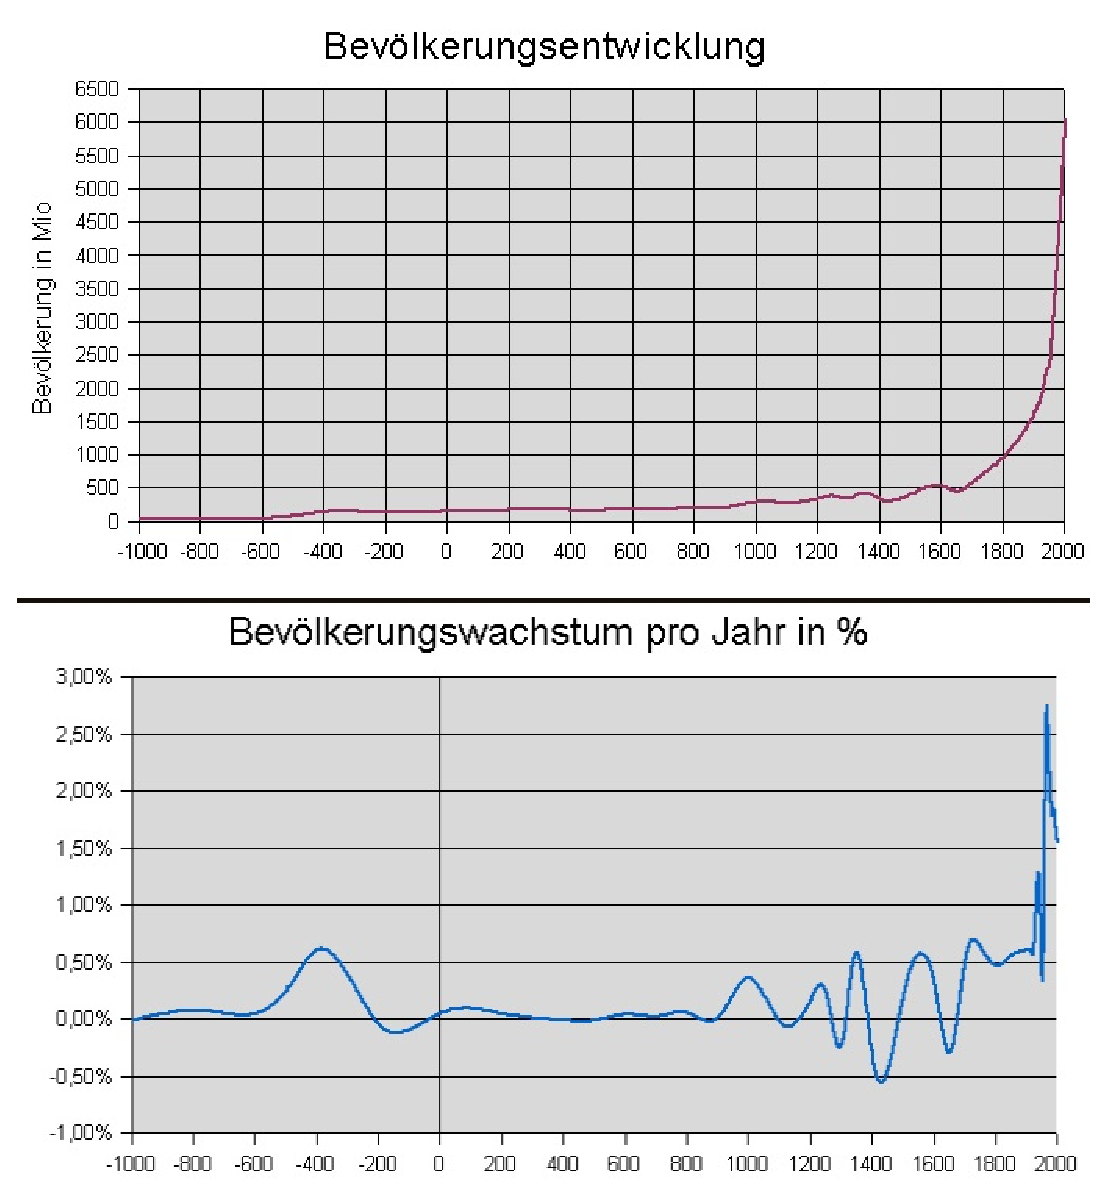
\includegraphics{../_database/Bilder/Bild24-1.eps}}
				\begin{tiny}Quelle: https://upload.wikimedia.org/wikipedia/commons/8/8a/World-pop-hist-de-2.png\end{tiny}
								
				\begin{scriptsize}Abbildung 1\end{scriptsize}
				\end{center}
				
				\meinlr{\resizebox{1\linewidth}{!}{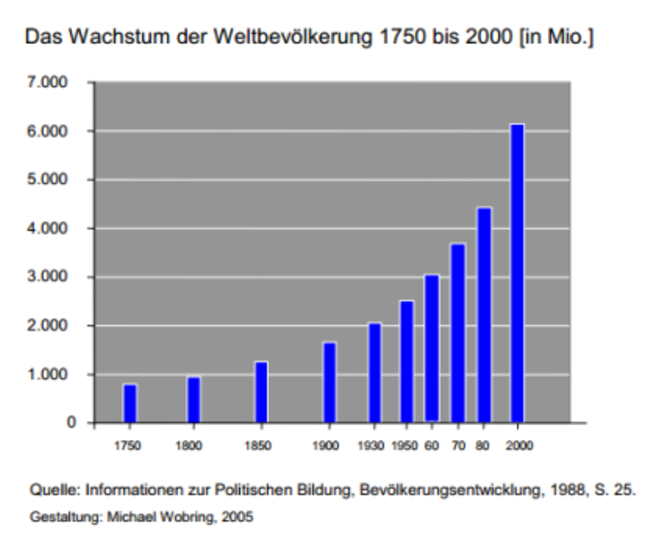
\includegraphics{../_database/Bilder/Bild24-2.eps}}
								\begin{center}\begin{scriptsize}Abbildung 2\end{scriptsize}\end{center}}{\resizebox{1.4\linewidth}{!}{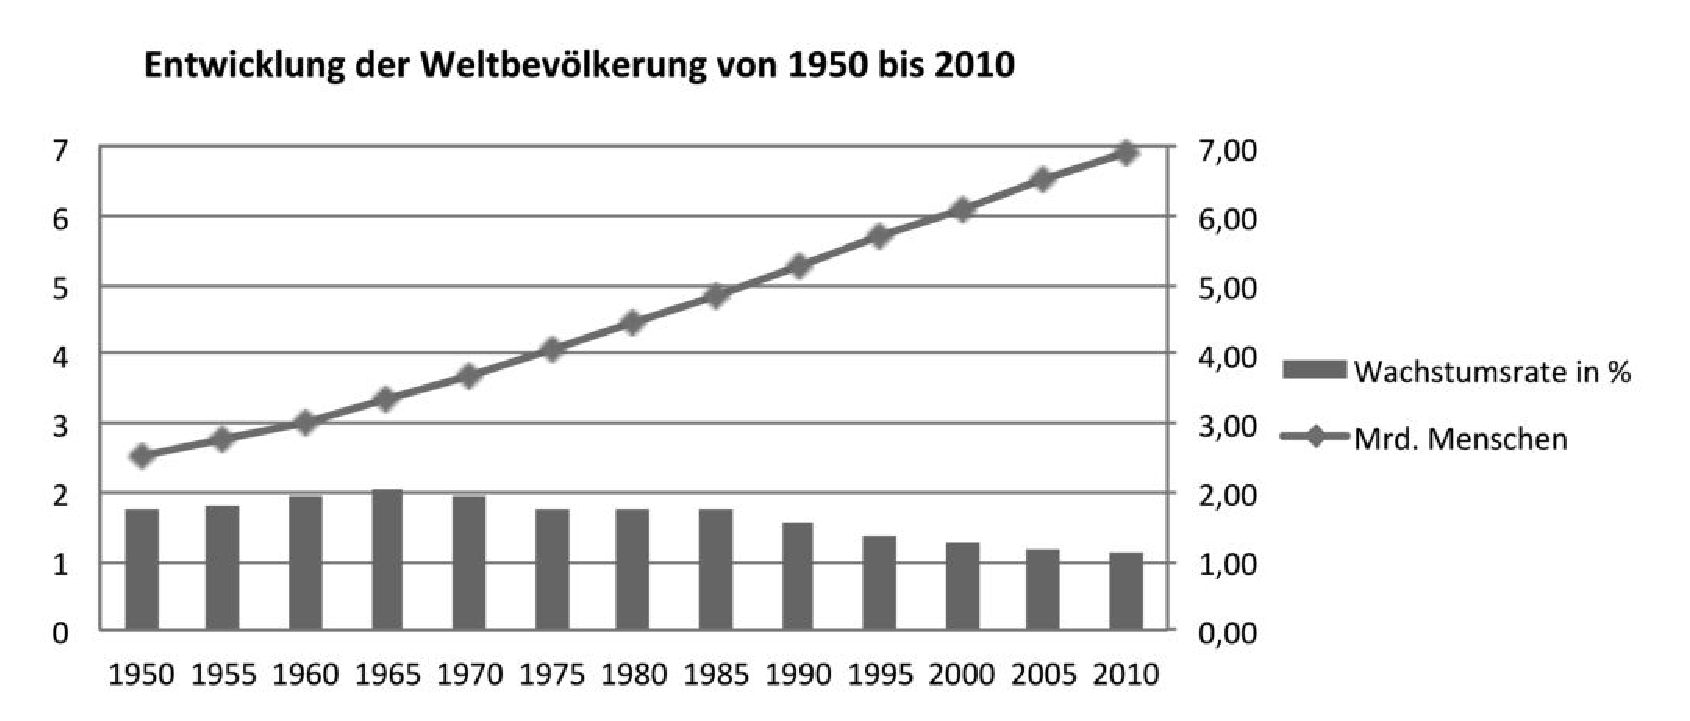
\includegraphics{../_database/Bilder/Bild24-3.eps}}
								\begin{center}\begin{scriptsize}Abbildung 3\end{scriptsize}\end{center}}\leer
								
				\begin{scriptsize}				
				\begin{tabular}{|C{1.7cm}|C{1.7cm}|C{1.7cm}|C{1.7cm}|C{1.7cm}|C{1.7cm}|C{1.7cm}|}\hline
				Jahr&Afrika&Asien&Europa&Lateinamerika&Nordamerika&Ozeanien\\ \hline
				1900&133&925&430&74&82&6\\ \hline
				1950&227&1\,403&547&167&172&13\\ \hline
				1975&419&2\,379&676&323&242&21\\ \hline
				2000&819&3\,698&727&521&319&31\\ \hline				
				\end{tabular}
				\end{scriptsize}

\subsection{Aufgabenstellung:}
\begin{enumerate}
	\item Ermittle anhand der Abbildungen, um wie viele Menschen die Weltbevölkerung von 1600 bis 18000 zugenommen hat!
	
	Nenne zwei Zeiträume, in denen die Weltbevölkerung mindesten 100 Jahre lang abgenommen hat, und begründe ihre Antwort!
	
	\item Die Weltbevölkerung hat von 1930 bis 1980 annähernd exponentiell zugenommen. Berechne unter dieser Annahme für diesen Zeitraum die jährliche Wachstumsrate auf Zehntelprozent genau!
	
	\item Begründe anhand der jährlichen Wachstumsraten aus Abbildung 3, warum die Entwicklung der Weltbevölkerung von 1950 bis 2010 nicht durch eine Exponentialfunktion beschrieben werden kann!
	
Bei konstanter Zunahme der Bevölkerungszahl ab 2010 wird für das Jahr 2050 eine Bevölkerungszahl von 10,4 Milliarden prognostiziert.\\
Berechne, von welcher jährlichen Zunahme bei dieser Prognose ausgegangen wird!
Gib die jährliche Zunahme in Millionen Menschen an!

\item Angenommen, die absoluten Zahlen der Bevölkerungsentwicklung der Kontinente und
Subkontinente im Zeitraum von 1900 bis 2000 werden in einem Säulendiagramm mit
linearer Skalierung dargestellt.\\
Begründe, warum die starke Bevölkerungszunahme in Ozeanien von 1900 bis 2000
in einem solchen Diagramm nicht erkennbar ist!

Gegeben sind fünf Aussagen zur Bevölkerungsentwicklung nach Kontinenten und Subkontinenten von 1900 bis 2000.\\
Kreuze die zutreffende(n) Aussage(n) an!\leer

\multiplechoice[5]{  %Anzahl der Antwortmoeglichkeiten, Standard: 5
				L1={Die Bevölkerung Asiens hat sich im 20. Jahrhundert annähernd
vervierfacht.},   %1. Antwortmoeglichkeit 
				L2={Seit Beginn des 20. Jahrhunderts lebten in Lateinamerika mehr
Menschen als in Nordamerika.},   %2. Antwortmoeglichkeit
				L3={Im Zeitraum von 1975 bis 2000 war die relative Bevölkerungszu-
nahme in Afrika am größten.},   %3. Antwortmoeglichkeit
				L4={In Europa war die Bevölkerungszunahme von 1975 bis 2000 ge-
ringer als von 1950 bis 1975.},   %4. Antwortmoeglichkeit
				L5={1950 lebten in Europa und Amerika zusammen bereits mehr als
eine Milliarde Menschen.},	 %5. Antwortmoeglichkeit
				L6={},	 %6. Antwortmoeglichkeit
				L7={},	 %7. Antwortmoeglichkeit
				L8={},	 %8. Antwortmoeglichkeit
				L9={},	 %9. Antwortmoeglichkeit
				%% LOESUNG: %%
				A1=1,  % 1. Antwort
				A2=3,	 % 2. Antwort
				A3=4,  % 3. Antwort
				A4=0,  % 4. Antwort
				A5=0,  % 5. Antwort
				}
						\end{enumerate}\leer
				
\antwort{\subsection{Lösungserwartung:}
\begin{enumerate}
	\item Zunahme von 1600 bis 1800: ca. 500 Millionen Menschen
	
	Die Weltbevölkerung hat mindestens 100 Jahre lang abgenommen in [250 v. Chr.; 50 v. Chr.] (bzw. $[-250;-50]$) und $[1400;1500]$, da in diesen Zeitintervallen das jährliche Bevölkerungswachstum in \% negativ ist.
	
	\item $N(t)=N_0\cdot a^t$\\
	$4,5=2\cdot a^50$\\
	$a\approx 1,016$, d.h. Zunahme um 1,6\,\% pro Jahr
	
	\item Bei einer exponentiellen Zunahme ist die jährliche Wachstumsrate konstant. Abbildung 3 zeigt, dass diese Voraussetzung im Zeitraum von 1950 bis 2010 nicht erfüllt ist.
	
	Konstante jährliche Zunahme von 2010 bis 2050:\\
	$\frac{10,4-6,9}{40}=0,0874$ Milliarden = 87,5 Millionen
	
	\item Da die Bevölkerungszahl Ozeaniens von 1900 bis 2000 jeweils weniger als 1\,\% der
Bevölkerungszahl Asiens betrug, sind die entsprechenden Säulen für Ozeanien sehr
niedrig (Höhe fast null).\\
Daher ist die Verfünffachung der Bevölkerungszahl Ozeaniens nicht erkennbar.

Lösung Multiple Choice siehe oben
			\end{enumerate}}
		\end{langesbeispiel}%
\hrule  \leer

\section{27 - MAT - AN 1.1, AN 1.3, FA 2.2, WS 1.2, WS 1.3, WS 1.1 - Kartoffeln in �sterreich - BIFIE Aufgabensammlung}

\begin{langesbeispiel} \item[0] %PUNKTE DES BEISPIELS
				Die Kartoffel ist weltweit eines der wichtigsten Nahrungsmittel.
				
				Die nachstehende Grafik zeigt die Entwicklung der Kartoffelerzeugung in �sterreich vom Jahr 2000 bis zum Jahr 2011.
				
				\begin{center}
					\textbf{Kartoffelerzeugung}
					
					\resizebox{0.8\linewidth}{!}{\psset{xunit=1.0cm,yunit=0.7cm,algebraic=true,dimen=middle,dotstyle=o,dotsize=5pt 0,linewidth=0.8pt,arrowsize=3pt 2,arrowinset=0.25}
\begin{pspicture*}(-1.366338441507557,-1.4071090537819535)(11.835465721609575,9.72757238201069)
\multips(0,0)(0,1.0){12}{\psline[linestyle=dashed,linecap=1,dash=1.5pt 1.5pt,linewidth=0.4pt,linecolor=lightgray]{c-c}(0,0)(11.835465721609575,0)}
\multips(0,0)(1.0,0){13}{\psline[linestyle=dashed,linecap=1,dash=1.5pt 1.5pt,linewidth=0.4pt,linecolor=lightgray]{c-c}(0,0)(0,9.72757238201069)}
\psaxes[labelFontSize=\scriptstyle,xAxis=true,yAxis=true,yLabels={,100, 200, 300, 400, 500, 600, 700, 800, 900},Ox=2000,Dx=1.,Dy=1.,ticksize=-2pt 0,subticks=2]{->}(0,0)(0.,0.)(11.835465721609575,9.72757238201069)
\psline[linewidth=1.2pt](0.,6.95)(1.,6.95)
\psline[linewidth=1.2pt](1.,6.95)(2.,6.84)
\psline[linewidth=1.2pt](2.,6.84)(3.,5.6)
\psline[linewidth=1.2pt](3.,5.6)(4.,6.93)
\psline[linewidth=1.2pt](4.,6.93)(5.,7.63)
\psline[linewidth=1.2pt](5.,7.63)(6.,6.55)
\psline[linewidth=1.2pt](6.,6.55)(7.,6.69)
\psline[linewidth=1.2pt](7.,6.69)(8.,7.57)
\psline[linewidth=1.2pt](8.,7.57)(9.,7.22)
\psline[linewidth=1.2pt](9.,7.22)(10.,6.72)
\psline[linewidth=1.2pt](10.,6.72)(11.,8.16)
\begin{scriptsize}
\rput[tl](-1,6){$\rotatebox{90}{\text{Menge in 1000 Tonnen}}$}
\rput[tl](0.02236339286879133,7.3){695}
\rput[tl](0.75,6.8){695}
\rput[tl](1.75,7.3){684}
\rput[tl](2.75,5.5){560}
\rput[tl](3.75,7.4){693}
\rput[tl](4.75,8){763}
\rput[tl](5.75,6.45){655}
\rput[tl](6.75,6.6){669}
\rput[tl](7.75,7.9){757}
\rput[tl](8.75,7.6){722}
\rput[tl](9.75,6.6){672}
\rput[tl](10.75,8.55){816}
\rput[tl](5.151545584806671,-0.8116715438465181){Jahr}
\end{scriptsize}
\end{pspicture*}}
				\end{center}\leer
				
				In der nachstehenden Abbildung werden Kartoffelexporte und -importe f�r den gleichen Zeitraum einander gegen�bergestellt.
				
				\begin{center}
					\textbf{Au�enhandel}
					
					\resizebox{0.8\linewidth}{!}{\newrgbcolor{qqzzff}{0. 0.6 1.}
\psset{xunit=1.0cm,yunit=0.3cm,algebraic=true,dimen=middle,dotstyle=o,dotsize=5pt 0,linewidth=0.8pt,arrowsize=3pt 2,arrowinset=0.25}
\begin{pspicture*}(-1.38,-3.449354157872534)(12.4,28.08759814267654)
\multips(0,-0)(0,5.0){7}{\psline[linestyle=dashed,linecap=1,dash=1.5pt 1.5pt,linewidth=0.4pt,linecolor=lightgray]{c-c}(0,0)(12.4,0)}
\multips(0,0)(1.0,0){14}{\psline[linestyle=dashed,linecap=1,dash=1.5pt 1.5pt,linewidth=0.4pt,linecolor=lightgray]{c-c}(0,0)(0,28.08759814267654)}
\psaxes[labelFontSize=\scriptstyle,xAxis=true,yAxis=true,yLabels={,50, 100, 150, 200, 250}, Ox=2000,Dx=1.,Dy=5.,ticksize=-2pt 0,subticks=2]{->}(0,0)(0.,0.)(12.4,28.08759814267654)
\psline[linewidth=1.2pt,linecolor=qqzzff](0.,8.4)(1.,9.1)
\psline[linewidth=1.2pt,linecolor=qqzzff](1.,9.1)(2.,12.9)
\psline[linewidth=1.2pt,linecolor=qqzzff](2.,12.9)(3.,13.5)
\psline[linewidth=1.2pt,linecolor=qqzzff](3.,13.5)(4.,11.9)
\psline[linewidth=1.2pt,linecolor=qqzzff](4.,11.9)(5.,12.8)
\psline[linewidth=1.2pt,linecolor=qqzzff](5.,12.8)(6.,16.4)
\psline[linewidth=1.2pt,linecolor=qqzzff](6.,16.4)(7.,17.7)
\psline[linewidth=1.2pt,linecolor=qqzzff](7.,17.7)(8.,15.4)
\psline[linewidth=1.2pt,linecolor=qqzzff](8.,15.4)(9.,18.2)
\psline[linewidth=1.2pt,linecolor=qqzzff](9.,18.2)(10.,19.8)
\psline[linewidth=1.2pt,linecolor=qqzzff](10.,19.8)(11.,17.2)
\psline[linewidth=1.2pt,linestyle=dashed,dash=7pt 7pt,linecolor=red](0.,7.5)(1.,6.6)
\psline[linewidth=1.2pt,linestyle=dashed,dash=7pt 7pt,linecolor=red](1.,6.6)(2.,9.)
\psline[linewidth=1.2pt,linestyle=dashed,dash=7pt 7pt,linecolor=red](2.,9.)(3.,8.2)
\psline[linewidth=1.2pt,linestyle=dashed,dash=7pt 7pt,linecolor=red](3.,8.2)(4.,10.2)
\psline[linewidth=1.2pt,linestyle=dashed,dash=7pt 7pt,linecolor=red](4.,10.2)(5.,14.8)
\psline[linewidth=1.2pt,linestyle=dashed,dash=7pt 7pt,linecolor=red](5.,14.8)(6.,13.2)
\psline[linewidth=1.2pt,linestyle=dashed,dash=7pt 7pt,linecolor=red](6.,13.2)(7.,13.2)
\psline[linewidth=1.2pt,linestyle=dashed,dash=7pt 7pt,linecolor=red](7.,13.2)(8.,17.1)
\psline[linewidth=1.2pt,linestyle=dashed,dash=7pt 7pt,linecolor=red](8.,17.1)(9.,17.2)
\psline[linewidth=1.2pt,linestyle=dashed,dash=7pt 7pt,linecolor=red](9.,17.2)(10.,16.7)
\psline[linewidth=1.2pt,linestyle=dashed,dash=7pt 7pt,linecolor=red](10.,16.7)(11.,20.8)
\psline[linewidth=1.2pt,linecolor=qqzzff](1.,24.)(2.,24.)
\psline[linewidth=1.2pt,linestyle=dashed,dash=7pt 7pt,linecolor=red](1.,22.)(2.,22.)
\begin{scriptsize}
\rput[tl](6.1,-1.8478682988602764){Jahr}
\rput[tl](0.1,9.5){\qqzzff{84}}
\rput[tl](0.85,10.5){\qqzzff{91}}
\rput[tl](1.8,14.1){\qqzzff{129}}
\rput[tl](2.8,14.6){\qqzzff{135}}
\rput[tl](3.8,13.25){\qqzzff{119}}
\rput[tl](4.8,12.5){\qqzzff{128}}
\rput[tl](5.8,17.65){\qqzzff{164}}
\rput[tl](6.8,18.7){\qqzzff{177}}
\rput[tl](7.8,15){\qqzzff{154}}
\rput[tl](8.8,19.45){\qqzzff{182}}
\rput[tl](9.8,20.8){\qqzzff{198}}
\rput[tl](10.8,16.9){\qqzzff{172}}
\rput[tl](0.1,6.9){\red{75}}
\rput[tl](0.85,6.3){\red{66}}
\rput[tl](1.85,10.1){\red{90}}
\rput[tl](2.85,8){\red{82}}
\rput[tl](3.8,9.7){\red{102}}
\rput[tl](4.8,16){\red{148}}
\rput[tl](5.8,12.9){\red{132}}
\rput[tl](6.8,12.9){\red{132}}
\rput[tl](7.8,18.2){\red{171}}
\rput[tl](8.8,16.8){\red{172}}
\rput[tl](9.8,16.5){\red{167}}
\rput[tl](10.8,21.8){\red{208}}
\rput[tl](2.4,24.5){\qqzzff{Kartoffelimporte}}
\rput[tl](2.4,22.5){\red{Kartoffelexporte}}
\rput[tl](-1.08,20.08016884761525){$\rotatebox{90}{\text{Menge in 1000 Tonnen}}$}
\end{scriptsize}
\end{pspicture*}}
					\end{center}

\subsection{Aufgabenstellung:}
\begin{enumerate}
	\item Entnehmen Sie der entsprechenden Graphik, zwischen welchen (aufeinanderfolgenden)
Jahren die absolute Zunahme (in Tonnen) und die relative Zunahme (in Prozent) der Erzeugung im Vergleich zum Vorjahr jeweils am gr��ten war! Gib die entsprechenden
Werte an!

Im vorliegenden Fall fand die gr��te relative Zunahme der Erzeugung in einem anderen
Zeitintervall statt als die gr��te absolute Zunahme.\\
Gib eine mathematische Begr�ndung an, warum die gr��te relative Zunahme und
die gr��te absolute Zunahme einer Gr��e oder eines Prozesses nicht im gleichen Zeitintervall stattfinden m�ssen!

\item Berechne und interpretiere den Ausdruck $\frac{E_{2011}-E_{2000}}{11}$, wobei $E_\text{Jahr}$ die Exportmenge in einem Kalenderjahr angibt! Gib bei der Interpretation auch die entsprechende Einheit an.

Die Exportentwicklung von 2000 bis 2011 soll durch eine lineare Funktion $f$ approximiert
werden, wobei die Variable t die Anzahl der seit 2000 vergangenen Jahre sein soll. Die
Funktionswerte f�r die Jahre 2000 und 2011 sollen dabei mit den in der Graphik angef�hrten Werten �bereinstimmen. Gib eine Gleichung dieser Funktion $f$ an!

\item Stelle in der nachstehenden Abbildung die Differenz "`Export minus Import"' der Mengen an Kartoffeln f�r die Jahre 2003 bis 2009 in einem S�ulendiagramm dar!
	
	\begin{center}
					\textbf{Saldo Export-Import}
					
					\resizebox{0.8\linewidth}{!}{\psset{xunit=1.4cm,yunit=0.05cm,algebraic=true,dimen=middle,dotstyle=o,dotsize=5pt 0,linewidth=0.8pt,arrowsize=3pt 2,arrowinset=0.25}
\begin{pspicture*}(-1,-69.33333333333154)(7.151969309462931,66.39999999999834)
\multips(0,-60)(0,4.0){34}{\psline[linestyle=dashed,linecap=1,dash=1.5pt 1.5pt,linewidth=0.4pt,linecolor=lightgray]{c-c}(0,0)(7.151969309462931,0)}
\multips(0,0)(100.0,0){1}{\psline[linestyle=dashed,linecap=1,dash=1.5pt 1.5pt,linewidth=0.4pt,linecolor=lightgray]{c-c}(0,-60)(0,66.39999999999834)}
\psaxes[labelFontSize=\scriptstyle,xAxis=true,yAxis=true,labels=y,Dx=1.,Dy=20.,ticksize=-2pt 0,subticks=2]{->}(0,0)(0.,-60)(7.151969309462931,66.39999999999834)
\antwort{\pspolygon[linecolor=blue,fillcolor=blue,fillstyle=solid,opacity=0.5](0.2,0.)(0.2,-53.)(0.8,-53.)(0.8,0.)
\pspolygon[linecolor=blue,fillcolor=blue,fillstyle=solid,opacity=0.5](1.2,0.)(1.2,-17.)(1.8,-17.)(1.8,0.)
\pspolygon[linecolor=blue,fillcolor=blue,fillstyle=solid,opacity=0.5](2.2,0.)(2.2,20.)(2.8,20.)(2.8,0.)
\pspolygon[linecolor=blue,fillcolor=blue,fillstyle=solid,opacity=0.5](3.2,0.)(3.2,-32.)(3.8,-32.)(3.8,0.)
\pspolygon[linecolor=blue,fillcolor=blue,fillstyle=solid,opacity=0.5](4.2,0.)(4.2,-45.)(4.8,-45.)(4.8,0.)
\pspolygon[linecolor=blue,fillcolor=blue,fillstyle=solid,opacity=0.5](5.2,0.)(5.2,17.)(5.8,17.)(5.8,0.)
\pspolygon[linecolor=blue,fillcolor=blue,fillstyle=solid,opacity=0.5](6.2,0.)(6.2,-10.)(6.8,-10.)(6.8,0.)}
\begin{scriptsize}
\rput[tl](0.3,-3.1999999999998883){2003}
\rput[tl](1.3,-3.1999999999998883){2004}
\rput[tl](2.3,-3.1999999999998883){2005}
\rput[tl](3.3,-3.1999999999998883){2006}
\rput[tl](4.3,-3.1999999999998883){2007}
\rput[tl](5.3,-3.1999999999998883){2008}
\rput[tl](6.3,-3.1999999999998883){2009}
\rput[tl](3,-63){Jahr}
\rput[tl](-0.8,26.93333333333268){$\rotatebox{90}{\text{Saldo in 1000 Tonnen}}$}
\end{scriptsize}
\end{pspicture*}}
\end{center}

Berechne das arithmetische Mittel dieser Differenz f�r die genannten Jahre!

\item Ein Index ist eine statistische Kennziffer, um die Entwicklung von Gr��en im Zeitverlauf darzustellen. Oft wird der Ausgangswert mit dem Basiswert 100 versehen. Ein Index von 120 bedeutet beispielsweise, dass eine Gr��e seit dem Basiszeitpunkt um 20\,\% gestiegen ist.

Die nachstehende Graphik zeigt die Entwicklung der in �sterreich verzehrten Kartoffelmenge (Nahrungsverbrauch) bezogen auf das Jahr 2000.

\begin{center}
					\textbf{Nahrungsverbrauch}
					
					\resizebox{0.8\linewidth}{!}{\psset{xunit=1.6cm,yunit=0.8cm,algebraic=true,dimen=middle,dotstyle=o,dotsize=5pt 0,linewidth=0.8pt,arrowsize=3pt 2,arrowinset=0.25}
\begin{pspicture*}(-0.8674067054466462,-1.1184701870029385)(6.267692353635041,8.521136170252973)
\multips(0,0)(0,1.0){10}{\psline[linestyle=dashed,linecap=1,dash=1.5pt 1.5pt,linewidth=0.4pt,linecolor=lightgray]{c-c}(0,0)(7.267692353635041,0)}
\multips(0,0)(100.0,0){1}{\psline[linestyle=dashed,linecap=1,dash=1.5pt 1.5pt,linewidth=0.4pt,linecolor=lightgray]{c-c}(0,0)(0,8.521136170252973)}
\psaxes[labelFontSize=\scriptstyle,xAxis=true,yAxis=true,labels=y,yLabels={,\text{94,0}, \text{96,0},\text{98,0},\text{100,0},\text{102,0},\text{104,0},\text{106,0},\text{108,0},\text{110,0}},Dx=1.,Dy=1.,ticksize=-2pt 0,subticks=2]{->}(0,0)(0.,0.)(6.267692353635041,8.521136170252973)
\pspolygon[linecolor=blue,fillcolor=blue,fillstyle=solid,opacity=1.0](0.25,0.)(0.25,3.)(0.5,3.)(0.5,0.)
\pspolygon[linecolor=red,fillcolor=red,fillstyle=solid,opacity=1.0](0.75,0.)(0.5,0.)(0.5,3.)(0.75,3.)
\pspolygon[linecolor=blue,fillcolor=blue,fillstyle=solid,opacity=1.0](1.25,0.)(1.25,5.1)(1.5,5.1)(1.5,0.)
\pspolygon[linecolor=red,fillcolor=red,fillstyle=solid,opacity=1.0](1.5,5.15)(1.75,5.15)(1.75,0.)(1.5,0.)
\pspolygon[linecolor=blue,fillcolor=blue,fillstyle=solid,opacity=1.0](2.25,0.)(2.25,4.)(2.5,4.)(2.5,0.)
\pspolygon[linecolor=red,fillcolor=red,fillstyle=solid,opacity=1.0](2.5,0.)(2.5,3.4)(2.75,3.4)(2.75,0.)
\pspolygon[linecolor=blue,fillcolor=blue,fillstyle=solid,opacity=1.0](3.25,0.)(3.25,3.9)(3.5,3.9)(3.5,0.)
\pspolygon[linecolor=red,fillcolor=red,fillstyle=solid,opacity=1.0](3.5,0.)(3.5,2.8)(3.75,2.8)(3.75,0.)
\pspolygon[linecolor=blue,fillcolor=blue,fillstyle=solid,opacity=1.0](4.25,0.)(4.25,7.2)(4.5,7.2)(4.5,0.)
\pspolygon[linecolor=red,fillcolor=red,fillstyle=solid,opacity=1.0](4.5,0.)(4.5,5.6)(4.75,5.6)(4.75,0.)
\pspolygon[linecolor=blue,fillcolor=blue,fillstyle=solid,opacity=1.0](5.25,0.)(5.25,6.05)(5.5,6.05)(5.5,0.)
\pspolygon[linecolor=red,fillcolor=red,fillstyle=solid,opacity=1.0](5.5,0.)(5.5,4.2)(5.75,4.2)(5.75,0.)
\pspolygon[linecolor=blue,fillcolor=blue,fillstyle=solid,opacity=1.0](0.25,8.)(0.25,7.5)(0.5,7.5)(0.5,8.)
\pspolygon[linecolor=red,fillcolor=red,fillstyle=solid,opacity=1.0](0.25,7.)(0.25,6.5)(0.5,6.5)(0.5,7.)
\begin{scriptsize}
\rput[tl](0.63,7.85){Nahrungsverbrauch}
\rput[tl](0.63,6.85){Nahrungsverbrauch pro Kopf}
\rput[tl](-0.8,6.949255369364486){$\rotatebox{90}{\text{Index bezogen auf das Jahr 2000}}$}
\rput[tl](3,-0.7){Jahr}
\rput[tl](0.3,-0.15){2000}
\rput[tl](1.3,-0.15){2002}
\rput[tl](2.3,-0.15){2004}
\rput[tl](3.3,-0.15){2006}
\rput[tl](4.3,-0.15){2008}
\rput[tl](5.3,-0.15){2010}
\end{scriptsize}
\end{pspicture*}}
\end{center}

Geben Sie jeweils ein Jahr an, in dem die Einwohnerzahl in �sterreich h�her bzw. niedriger
war als im Jahr 2000! Begr�nde deine Antwort!

Zeichne in die nachstehende Graphik zwei m�gliche S�ulen f�r ein Jahr, in dem der
absolute Nahrungsverbrauch niedriger und die Bev�lkerungszahl h�her war als im
Jahr 2000!

\begin{center}
					\textbf{Nahrungsverbrauch}
					
					\resizebox{0.8\linewidth}{!}{\psset{xunit=5cm,yunit=0.8cm,algebraic=true,dimen=middle,dotstyle=o,dotsize=5pt 0,linewidth=0.8pt,arrowsize=3pt 2,arrowinset=0.25}
\begin{pspicture*}(-0.35,-1.1184701870029385)(2.267692353635041,11.521136170252973)
\multips(0,0)(0,1.0){12}{\psline[linestyle=dashed,linecap=1,dash=1.5pt 1.5pt,linewidth=0.4pt,linecolor=lightgray]{c-c}(0,0)(7.267692353635041,0)}
\multips(0,0)(100.0,0){1}{\psline[linestyle=dashed,linecap=1,dash=1.5pt 1.5pt,linewidth=0.4pt,linecolor=lightgray]{c-c}(0,0)(0,8.521136170252973)}
\psaxes[labelFontSize=\scriptstyle,xAxis=true,yAxis=true,labels=y,yLabels={,\text{0,0}, \text{20,0},\text{40,0},\text{60,0},\text{80,0},\text{100,0},\text{120,0},\text{140,0},\text{160,0},\text{180,0},\text{200,0}},Dx=1.,Dy=1.,ticksize=-2pt 0]{->}(0,0)(0.,0.)(2.267692353635041,11.521136170252973)
\pspolygon[linecolor=blue,fillcolor=blue,fillstyle=solid,opacity=1.0](0.25,0.)(0.25,3.)(0.5,3.)(0.5,0.)
\pspolygon[linecolor=red,fillcolor=red,fillstyle=solid,opacity=1.0](0.75,0.)(0.5,0.)(0.5,3.)(0.75,3.)

\pspolygon[linecolor=blue,fillcolor=blue,fillstyle=solid,opacity=1.0](0.25,11.)(0.25,10.5)(0.35,10.5)(0.35,11.)
\pspolygon[linecolor=red,fillcolor=red,fillstyle=solid,opacity=1.0](0.25,10.)(0.25,9.5)(0.35,9.5)(0.35,10.)
\begin{scriptsize}
\rput[tl](0.4,10.85){Nahrungsverbrauch}
\rput[tl](0.4,9.85){Nahrungsverbrauch pro Kopf}
\rput[tl](-0.25,7.6){$\rotatebox{90}{\text{Index bezogen auf das Jahr 2000}}$}
\rput[tl](1,-0.4){Jahr}
\rput[tl](0.44,-0.15){2000}
\rput[tl](1.44,-0.15){2002}
\end{scriptsize}
\end{pspicture*}}
\end{center}
						\end{enumerate}\leer
				
\antwort{\subsection{L�sungserwartung:}
\begin{enumerate}
	\item absolute Zunahme zwischen 2003 und 2004: 133 000 Tonnen\\
absolute Zunahme zwischen 2010 und 2011: 144 000 Tonnen\\
Die gr��te absolute Zunahme war im Zeitintervall von 2010 bis 2011.\\
relative Zunahme zwischen 2003 und 2004: 23,75\,\%\\
L�sungsintervall in Prozent: $[23; 24]$\\
relative Zunahme zwischen 2010 und 2011: ca. 21,43\,\%\\
L�sungsintervall in Prozent: $[21; 22]$
Die gr��te relative Zunahme war zwischen 2003 und 2004.\\
Da f�r die Berechnung der relativen Zunahme einer Gr��e auch der Bezugswert entscheidend ist, m�ssen gr��te absolute Zunahme und gr��te relative Zunahme einer Gr��e oder
eines Prozesses nicht im gleichen Zeitintervall stattfinden. �quivalente Formulierungen sind
ebenfalls als richtig zu werten.

\item $\frac{E_{2011}-E_{2000}}{11}\approx 12\,000$ Tonnen pro Jahr.

Die durchschnittliche Zunahme des �sterreichischen Kartoffelexports betr�gt
ca. 12 000 Tonnen pro Jahr.\\
L�sungsintervall: $[12 000; 12 100]$
Die richtige Einheit muss in der Interpretation vorhanden sein.\\
$f$ mit $f(t)=75000+12000\cdot t$ oder $f(t)=75+12\cdot t$ oder $f(t)=\frac{133}{11}\cdot t+75$
Jede j�hrliche Zunahme aus dem oben angef�hrten L�sungsintervall muss akzeptiert werden.

\item L�sung Grafik siehe oben

Genauigkeit der S�ulenl�ngen: Toleranzbereich $\pm 5\,000$ Tonnen

arithmetisches Mittel: $\frac{-53-17+20-32-45+17-10}{7}\approx -17$

L�sungsintervall: bei Berechnung in 1\,000 Tonnen: $[-18; -16]$; bei Berechnung in Tonnen:
$[-18\,000; -16\,000]$
	
\item \begin{itemize}
	\item niedrigere Einwohnerzahl (als im Jahr 2000) in den Jahren: 2002 (prozentuelle Ver�nderung des Nahrungsverbrauchs kleiner als jene des Nahrungsverbrauchs pro Kopf)
\item h�here Einwohnerzahl (als im Jahr 2000) in den Jahren: 2004, 2006, 2008 und 2010
(prozentuelle Ver�nderung des Nahrungsverbrauchs gr��er als jene des Nahrungsverbrauchs pro Kopf)
\end{itemize}
Die Angabe eines Jahres ist hier ausreichend.

Die S�ule f�r den gesamten Nahrungsverbrauch muss niedriger sein als die S�ule f�r
100\% im Jahr 2000. Die S�ule f�r den Nahrungsverbrauch pro Kopf muss bei einer steigenden Bev�lkerungszahl niedriger als die S�ule f�r den gesamten Nahrungsverbrauch
sein.
			\end{enumerate}}
		\end{langesbeispiel}%
\hrule  \leer

\section{30 - MAT - AG 2.1, FA 4.1, FA 4.3, FA 5.1, FA 5.6, AN 1.1, AN 1.4, WS 1.3 - Waldbewirtschaftung - BIFIE Aufgabensammlung}

\begin{langesbeispiel} \item[0] %PUNKTE DES BEISPIELS
				Der Holzbestand eines durchschnittlichen Fichtenwaldes in Österreich beträgt $350\,m³$ pro Hektar Waldfläche. Pro Jahr ist mit einem durchschnittlichen Zuwachs von $3,3\,\%$ zu rechnen. Bei einer nachhaltigen Bewirtschaftung, wie sie in Österreich vorgeschrieben ist, soll der Holzbestand des Waldes gleich bleiben oder leicht zunehmen.
				
Der nachstehenden Grafik kann die Entwicklung des Holzpreises bei Fichtenholz im Zeitraum von 1995 bis 2011 entnommen werden.

\begin{center}
\subsection{Holzpreis bei Fichtenholz in \euro$/m³$}
\resizebox{1\linewidth}{!}{\psset{xunit=2.3cm,yunit=0.25cm,algebraic=true,dimen=middle,dotstyle=o,dotsize=5pt 0,linewidth=0.8pt,arrowsize=3pt 2,arrowinset=0.25}
\begin{pspicture*}(-0.82,-3.166666666666629)(9.52,49.66666666666655)
\multips(0,0)(0,2.0){27}{\psline[linestyle=dashed,linecap=1,dash=1.5pt 1.5pt,linewidth=0.4pt,linecolor=lightgray]{c-c}(0,0)(9.52,0)}
\multips(0,0)(100.0,0){1}{\psline[linestyle=dashed,linecap=1,dash=1.5pt 1.5pt,linewidth=0.4pt,linecolor=lightgray]{c-c}(0,0)(0,49.66666666666655)}
\psaxes[labelFontSize=\scriptstyle,xAxis=true,yAxis=true,labels=y,Oy=50,Dy=2.,ticksize=-2pt 0,subticks=2]{->}(0,0)(0.,0.)(9.52,49.66666666666655)
\rput[tl](0.06,48.749999999999886){\euro$/m³$}
\rput[tl](8.42,2.){Jahr}
\psline[linewidth=1.2pt](0.5,26.)(1.,14.)
\psline[linewidth=1.2pt](1.,14.)(1.5,23.)
\psline[linewidth=1.2pt](1.5,23.)(2.,28.)
\psline[linewidth=1.2pt](2.,28.)(2.5,29.)
\psline[linewidth=1.2pt](2.5,29.)(3.,23.)
\psline[linewidth=1.2pt](3.,23.)(3.5,23.)
\psline[linewidth=1.2pt](3.5,23.)(4.,24.)
\psline[linewidth=1.2pt](4.,24.)(4.5,16.)
\psline[linewidth=1.2pt](4.5,16.)(5.,18.)
\psline[linewidth=1.2pt](5.,18.)(5.5,19.)
\psline[linewidth=1.2pt](5.5,19.)(6.,26.)
\psline[linewidth=1.2pt](6.,26.)(6.5,26.)
\psline[linewidth=1.2pt](6.5,26.)(7.,19.)
\psline[linewidth=1.2pt](7.,19.)(7.5,20.)
\psline[linewidth=1.2pt](7.5,20.)(8.,39.)
\psline[linewidth=1.2pt](8.,39.)(8.5,44.)
\begin{scriptsize}
\psdots[dotsize=4pt 0,dotstyle=square*,dotangle=45](0.5,26.)
\psdots[dotsize=4pt 0,dotstyle=square*,dotangle=45](1.,14.)
\psdots[dotsize=4pt 0,dotstyle=square*,dotangle=45](1.5,23.)
\psdots[dotsize=4pt 0,dotstyle=square*,dotangle=45](2.,28.)
\psdots[dotsize=4pt 0,dotstyle=square*,dotangle=45](2.5,29.)
\psdots[dotsize=4pt 0,dotstyle=square*,dotangle=45](3.,23.)
\psdots[dotsize=4pt 0,dotstyle=square*,dotangle=45](3.5,23.)
\psdots[dotsize=4pt 0,dotstyle=square*,dotangle=45](4.,24.)
\psdots[dotsize=4pt 0,dotstyle=square*,dotangle=45](4.5,16.)
\psdots[dotsize=4pt 0,dotstyle=square*,dotangle=45](5.,18.)
\psdots[dotsize=4pt 0,dotstyle=square*,dotangle=45](5.5,19.)
\psdots[dotsize=4pt 0,dotstyle=square*,dotangle=45](6.,26.)
\psdots[dotsize=4pt 0,dotstyle=square*,dotangle=45](6.5,26.)
\psdots[dotsize=4pt 0,dotstyle=square*,dotangle=45](7.,19.)
\psdots[dotsize=4pt 0,dotstyle=square*,dotangle=45](7.5,20.)
\psdots[dotsize=4pt 0,dotstyle=square*,dotangle=45](8.,39.)
\psdots[dotsize=4pt 0,dotstyle=square*,dotangle=45](8.5,44.)
\rput[tl](-0.18,-1){1994}
\rput[tl](0.82,-1){1996}
\rput[tl](1.82,-1){1998}
\rput[tl](2.82,-1){2000}
\rput[tl](3.82,-1){2002}
\rput[tl](4.82,-1){2004}
\rput[tl](5.82,-1){2006}
\rput[tl](6.82,-1){2008}
\rput[tl](7.82,-1){2010}
\rput[tl](8.82,-1){2012}
\end{scriptsize}
\end{pspicture*}}
\end{center}

\subsection{Aufgabenstellung:}
\begin{enumerate}
	\item Bestimme das maximale Holzvolumen (in $m³/ha$), das bei einer nachhaltigen Bewirtschaftung pro Jahr geschlägert werden darf!
	
Berechne, um wie viel Prozent der Holzbestand eines durchschnittlichen Fichtenwaldes innerhalb von 10 Jahren zunimmt, unter der Annahme, dass keinerlei Schlägerungen vorgenommen werden, alle anderen genannten Rahmenbedingungen jedoch unverändert bleiben!

\item Der Holzbestand eines 20 ha großen Fichtenwaldes wird in einem Zeitraum von 15 Jahren jährlich jeweils am Ende des Jahres (nachdem der jährliche Zuwachs abgeschlossen ist) um 10 $m³$ pro Hektar (also um 200 $m³$) verringert.

Ermitteln Sie den Holzbestand des Fichtenwaldes nach Ablauf von 15 Jahren!

Gib an, ob bei dieser Art der Bewirtschaftung der Holzbestand des Fichtenwaldes trotz Schlägerung exponentiell zunimmt, und begründe deine Entscheidung!
	
\item Ermittel für den Zeitraum 2003 bis 2011 die empirische Standardabweichung des Holzpreises entsprechend der Formel

$$\sigma=\sqrt{\frac{1}{n-1}\cdot\sum^n_{i=1}({x_i-\overline{x})²}}$$

Dabei werden mit $x_i$ die Beobachtungswerte und mit $\overline{x}$ das arithmetische Mittel der Beobachtungswerte bezeichnet. Lies die dazu notwendigen Daten aus der Grafik ab!

Begründen Sie anhand der Grafik, warum die empirische Standardabweichung des
Holzpreises für den Zeitraum 1998 bis 2004 kleiner ist als die empirische Standardabweichung für den Zeitraum 2005 bis 2011!

\item Die Entwicklung des Holzpreises soll für den Zeitraum von 2009 bis 2011 durch eine Funktion $P$ mit $P(t)=a\cdot t²+b\cdot t+c$ mit $a,b,c\in\mathbb{R}$ und $a\neq 0$ modelliert werden. Der Holzpreis $P(t)$ wird in \euro$/m³$ angegeben, die Zeitrechnung beginnt mit dem Jahr 2009 und erfolgt in der Einheit "`Jahre"'.

Führe die Modellierung auf Basis der Daten für die Jahre 2009, 2010 und 2011 durch und begründe, warum der Parameter $a$ negativ sein muss!

Ermittle eine Prognose für den in der Grafik nicht angegebenen Holzpreis für das Jahr 2012 mithilfe dieser Modellfunktion!

\item Bestimme für den Zeitraum von 1995 bis 2011 die absoluten Holzpreisänderungen aufeinanderfolgender Jahre!

Gib dasjenige Intervall [Jahr 1; Jahr 2] an, in dem sich der Holzpreis prozentuell am stärksten ändert!
						\end{enumerate}\leer
				
\antwort{\subsection{Lösungserwartung:}
\begin{enumerate}
	\item $350\cdot 0,033=11,55$\\
	Jährlich dürfen bei einer nachhaltigen Bewirtschaftung maximal 11,55 $m³$/ha Holz geschlägert werden.
	
	$1,033^{10}\approx 1,384$\\
	Unter der Annahme, dass keine Schlägerungen erfolgen, nimmt der Holzbestand innerhalb von zehn Jahren um ca. 38,4\,\% zu.
	
	\item Tabelle:
	
	\begin{tabular}{|c|c|}\hline
	Jahr&Holzbestand in $m³$\\ \hline
	0&7\,000\\ \hline
	1&7\,031\\ \hline
	2&7\,063,023\\ \hline
	3&7\,096,102759\\ \hline
4&7\,130,27415\\ \hline
5&7\,165,573197\\ \hline
6&7\,202,037112\\ \hline
7&7\,239,704337\\ \hline
8&7\,278,61458\\ \hline
9&7\,318,808861\\ \hline
10&7\,360,329554\\ \hline
11&7\,403,220429\\ \hline
12&7\,447,526703\\ \hline
13&7\,493,295085\\ \hline
14&7\,540,573822\\ \hline
15&7\,589,412759\\ \hline
	\end{tabular}\leer
	
	Wenn der Holzbestand eines 20 ha großen Fichtenwaldes jährlich jeweils am Ende des Jahres um 10 $m³$ pro Hektar verringert wird, beträgt er nach Ablauf von 15 Jahren ca. 7 589,41 $m³$.
	
Bei dieser Art der Bewirtschaftung nimmt der Holzbestand nicht exponentiell zu, da das jährliche prozentuelle Wachstum nicht konstant ist.

\item Die empirische Standardabweichung beträgt ca. 9,91 \euro$/m³$.

Im Zeitraum von 1998 bis 2004 ist die empirische Standardabweichung des Holzpreises kleiner als im Zeitraum von 2005 bis 2011, da die Schwankungen der Werte des Holzpreises im Zeitraum von 1998 bis 2004 geringer sind.

\item $P(t)=-7\cdot t²+26\cdot t+70$

\begin{center}
	\subsection{Holzpreis in \euro$/m^3$}
	
	\resizebox{0.8\linewidth}{!}{\psset{xunit=5cm,yunit=0.09cm,algebraic=true,dimen=middle,dotstyle=o,dotsize=5pt 0,linewidth=0.8pt,arrowsize=3pt 2,arrowinset=0.25}
\begin{pspicture*}(-0.2473684210526314,-12.595999999999828)(2.9368421052631564,109.31528571428521)
\multips(0,0)(0,10.0){13}{\psline[linestyle=dashed,linecap=1,dash=1.5pt 1.5pt,linewidth=0.4pt,linecolor=lightgray]{c-c}(0,0)(2.9368421052631564,0)}
\multips(0,0)(10.0,0){1}{\psline[linestyle=dashed,linecap=1,dash=1.5pt 1.5pt,linewidth=0.4pt,linecolor=lightgray]{c-c}(0,0)(0,109.31528571428521)}
\psaxes[labelFontSize=\scriptstyle,xAxis=true,yAxis=true,Dx=0.5,Dy=10.,ticksize=-2pt 0,subticks=2]{->}(0,0)(0.,0.)(2.9368421052631564,109.31528571428521)
\psplot[linewidth=1.2pt,plotpoints=200]{0}{2}{-7.0*x^(2.0)+26.0*x+70.0}
\rput[tl](1.2052631578947361,-5.9){Jahre ab 2009}
\rput[tl](0.10526315789473682,104.36685714285666){$y=-7x²+26x+70$}
\rput[tl](0.32631578947368406,95.19349999999955){$R²=1$}
\begin{scriptsize}
\psdots[dotsize=4pt 0,dotstyle=square*,dotangle=45](0.,70.)
\psdots[dotsize=4pt 0,dotstyle=square*,dotangle=45](1.,89.)
\psdots[dotsize=4pt 0,dotstyle=square*,dotangle=45](2.,94.)
\end{scriptsize}
\end{pspicture*}}
\end{center}\leer

Der Wert des Parameters $a$ muss negativ sein, weil der Graph der Modellfunktion eine nach unten geöffnete Parabel ist.

Prognosewert für das Jahr 2012:\\
$P(3)=85\,$\euro$/m^3$

\item Tabelle:

\begin{tabular}{|c|c|c|c|}\hline
Jahr&Holzpreis in \euro$/m^3$&absolute Änderungen&prozentuelle Änderungen\\ \hline
1995&76& & \\ \hline
1996&64&-12&-15,79\\ \hline
1997&73&9&14,06\\ \hline
1998&78&5&6,85\\ \hline
1999&79&1&1,28\\ \hline
2000&73&-6&-7,59\\ \hline
2001&73&0&0\\ \hline
2002&74&1&1,37\\ \hline
2003&66&-8&-10,81\\ \hline
2004&68&2&3,03\\ \hline
2005&69&1&1,47\\ \hline
2006&76&7&10,14\\ \hline
2007&76&0&0\\ \hline
2008&69&-7&-9,21\\ \hline
2009&70&1&1,45\\ \hline
2010&89&19&27,14\\ \hline
2011&94&5&5,62\\ \hline
\end{tabular}\leer

Im Zeitraum $[2009; 2010]$ ändert sich der Holzpreis prozentuell am stärksten.
	\end{enumerate}}
		\end{langesbeispiel}%
\hrule  \leer

\section{31 - MAT - WS 1.1, WS 1.3 - Hallenbad - Matura 2013/14 Haupttermin}

\begin{langesbeispiel} \item[0] %PUNKTE DES BEISPIELS
				Das örtliche Hallenbad einer kleinen Gemeinde veröffentlicht Anfang 2008 in der Gemeindezeitschrift eine Statistik über die jährlichen Besucherzahlen und die Anzahl der offenen Tage für die letzten acht Jahre:
					
					\resizebox{1\linewidth}{!}{\begin{tabular}{|l|c|c|c|c|c|c|c|c|}\hline
					Jahr&2000&2001&2002&2003&2004&2005&2006&2007\\ \hline
					Besucherzahlen&33\,200&32\,500&34\,000&33\,500&33\,200&33\,100&32\,900&32\,500\\ \hline
					offene Tage&197&192&200&195&193&190&186&180\\ \hline
					\end{tabular}}

Das Hallenbad bedarf einer Renovierung. Im Gemeinderat steht nun die Entscheidung an, ob Geld in das Hallenbad investiert oder das Hallenbad geschlossen werden soll. Im Vorfeld der Entscheidung veröffentlichen zwei örtliche Gemeinderatsparteien - Partei $A$ und Partei $B$ - folgende Diagramme in ihren Parteizeitschriften:

\begin{center}
\textbf{Besucherzahlen 2000-2007}\leer

\resizebox{0.5\linewidth}{!}{\psset{xunit=1.0cm,yunit=0.15cm,algebraic=true,dimen=middle,dotstyle=o,dotsize=5pt 0,linewidth=0.8pt,arrowsize=3pt 2,arrowinset=0.25}
\begin{pspicture*}(-1.6848,-4.089123900293161)(8.8938,44.10412206744805)
\multips(0,0)(0,5.0){10}{\psline[linestyle=dashed,linecap=1,dash=1.5pt 1.5pt,linewidth=0.4pt,linecolor=lightgray]{c-c}(0,0)(8.8938,0)}
\multips(0,0)(1.0,0){11}{\psline[linestyle=dashed,linecap=1,dash=1.5pt 1.5pt,linewidth=0.4pt,linecolor=lightgray]{c-c}(0,0)(0,44.10412206744805)}
\psaxes[labelFontSize=\scriptstyle,xAxis=true,yAxis=true,showorigin=false,ylabelFactor={\,000}, Ox=1999,Dx=1.,Dy=5.,ticksize=-2pt 0,subticks=2]{->}(0,0)(0.,0.)(8.8938,44.10412206744805)
\psline(1.,33.2)(2.,32.5)
\psline(2.,32.5)(3.,34.)
\psline(3.,34.)(4.,33.5)
\psline(4.,33.5)(5.,33.2)
\psline(5.,33.2)(6.,33.1)
\psline(6.,33.1)(7.,32.9)
\psline(7.,32.9)(8.,32.5)
\begin{scriptsize}
\psdots[dotsize=3pt 0,dotstyle=square*,dotangle=45](1.,33.2)
\psdots[dotsize=3pt 0,dotstyle=square*,dotangle=45](2.,32.5)
\psdots[dotsize=3pt 0,dotstyle=square*,dotangle=45](3.,34.)
\psdots[dotsize=3pt 0,dotstyle=square*,dotangle=45](4.,33.5)
\psdots[dotsize=3pt 0,dotstyle=square*,dotangle=45](5.,33.2)
\psdots[dotsize=3pt 0,dotstyle=square*,dotangle=45](6.,33.1)
\psdots[dotsize=3pt 0,dotstyle=square*,dotangle=45](7.,32.9)
\psdots[dotsize=3pt 0,dotstyle=square*,dotangle=45](8.,32.5)
\end{scriptsize}
\end{pspicture*}}

\textit{Partei $A$}
\end{center}

\begin{center}
\textbf{Besucherzahlen 2000-2007}\leer

\resizebox{0.5\linewidth}{!}{\psset{xunit=1.0cm,yunit=2cm,algebraic=true,dimen=middle,dotstyle=o,dotsize=5pt 0,linewidth=0.8pt,arrowsize=3pt 2,arrowinset=0.25}
\begin{pspicture*}(0,31.9)(8.8938,34.4)
\multips(0,32.2)(0,0.4){10}{\psline[linestyle=dashed,linecap=1,dash=1.5pt 1.5pt,linewidth=0.4pt,linecolor=lightgray]{c-c}(2,0)(8.8938,0)}
\multips(2,0)(1.0,0){11}{\psline[linestyle=dashed,linecap=1,dash=1.5pt 1.5pt,linewidth=0.4pt,linecolor=lightgray]{c-c}(0,32.2)(0,44.10412206744805)}
\psaxes[labelFontSize=\scriptstyle,xAxis=true,yAxis=true,showorigin=false,labels=x,Ox=1999,Dx=1.,Dy=0.4,ticksize=-2pt 0]{->}(2,32.2)(2.,32.45)(8.8938,44.10412206744805)
\pszigzag[coilarm=0.125,coilwidth=0.3,coilheight=0.5](2,32.2)(2,32.5)
\psline(3.,34.)(4.,33.5)
\psline(4.,33.5)(5.,33.2)
\psline(5.,33.2)(6.,33.1)
\psline(6.,33.1)(7.,32.9)
\psline(7.,32.9)(8.,32.5)
\begin{scriptsize}
\psdots[dotsize=3pt 0,dotstyle=square*,dotangle=45](3.,34.)
\psdots[dotsize=3pt 0,dotstyle=square*,dotangle=45](4.,33.5)
\psdots[dotsize=3pt 0,dotstyle=square*,dotangle=45](5.,33.2)
\psdots[dotsize=3pt 0,dotstyle=square*,dotangle=45](6.,33.1)
\psdots[dotsize=3pt 0,dotstyle=square*,dotangle=45](7.,32.9)
\psdots[dotsize=3pt 0,dotstyle=square*,dotangle=45](8.,32.5)
\rput[tl](1,32.65){32\,400}
\rput[tl](1,33.05){32\,800}
\rput[tl](1,33.45){33\,200}
\rput[tl](1,33.85){33\,600}
\rput[tl](1,34.25){34\,000}
\end{scriptsize}
\end{pspicture*}}

\textit{Partei $B$}
\end{center}


\subsection{Aufgabenstellung:}
\begin{enumerate}
	\item Gib für jede Partei eine passende Botschaft an, wie mit dem jeweiligen Diagramm bezogen auf die Entwicklung der Besucherzahlen transportiert werden soll!\leer
		
		Partei $A$: \rule{5cm}{0.3pt}\leer
		
		Partei $B$: \rule{5cm}{0.3pt}\leer
		
		\item Partei $B$ hat bei der grafischen Darstellung verschiedene Manipulationen eingesetzt, um die Entwicklung der Besucherzahlen aus ihrer Sicht darzustellen.
		
 Beschreibe zwei dieser angewandten Manipulationen!\leer

\item \framebox[5mm][c]{A} Ermittle die Besucherzahlen pro Öffnungstag (gerundet auf ein eine Nachkommastelle) für die entsprechenden Jahre!\leer

\resizebox{1\linewidth}{!}{\begin{tabular}{|l|c|c|c|c|c|c|c|c|}\hline
Jahr&2000&2001&2002&2003&2004&2005&2006&2007\\ \hline
BesucherInnen&&&&&&&&\\
pro Tag&&&&&&&&\\ \hline
\end{tabular}}\leer

Formuliere eine dazu passende Aussage in Bezug auf die bevorstehende Entscheidung im Gemeinderat!

						\end{enumerate}\leer
				
\antwort{
\begin{enumerate}
	\item \subsection{Lösungserwartung:} 
	
	Partei $A$:  Das Hallenbad muss renoviert werden, da die Besucherzahlen über die letzten Jahre annähernd konstant geblieben sind.
	
	Partei $B$:   Das Hallenbad soll nicht renoviert werden, da die Besucherzahlen in den letzten Jahren stark abgenommen haben.
	
	\subsection{Lösungsschlüssel:}
	\begin{itemize}
		\item  Ein Punkt für eine richtige Aussage zu Partei $A$. 
		\item Ein Punkt für eine richtige Aussage zu Partei $B$.
		
		Zulässig sind auch andere Formulierungen, die den Kern der Aussagen treffen.
	\end{itemize}
	
	\item \subsection{Lösungserwartung:}
	\begin{itemize}
		\item Die senkrechte Achse beginnt bei null, allerdings ist der erste Abschnitt bis zum ersten  Skalierungswert verkürzt dargestellt. 
		\item Änderung/"'Verfeinerung"' der Skalierung
		\item Die x-Achsen-Skala beginnt mit 2002, daher fällt "`der ansteigende Teil"' in der Graphik weg (vgl. Anstieg der Besucherzahlen lt. Partei $A$).
	\end{itemize}
	
	\subsection{Lösungsschlüssel:}
	Zwei Punkte: je ein Punkt für eine (sinngemäß) korrekt angeführte Manipulation.
	
	\item \subsection{Lösungserwartung:} 
	\resizebox{1\linewidth}{!}{\begin{tabular}{|l|c|c|c|c|c|c|c|c|}\hline
Jahr&2000&2001&2002&2003&2004&2005&2006&2007\\ \hline
BesucherInnen&\multirow{2}{*}{168,5}&\multirow{2}{*}{169,3}&\multirow{2}{*}{170,0}&\multirow{2}{*}{171,8}&\multirow{2}{*}{172,0}&\multirow{2}{*}{174,2}&\multirow{2}{*}{176,9}&\multirow{2}{*}{180,6}\\
pro Tag&&&&&&&&\\ \hline
\end{tabular}}\leer

Investitionen in das Hallenbad lohnen sich, denn in den letzten acht Jahren stieg die Zahl der täglichen Besucher/innen jedes Jahr an.

\subsection{Lösungsschlüssel:}
\begin{itemize}
	\item Ein Ausgleichspunkt für die richtigen Werte in der Tabelle. Die Angabe einer Null nach dem Komma (z. B.: 170,0) kann entfallen.
	\item Ein Punkt für eine (sinngemäß) korrekte Antwort
\end{itemize}
\end{enumerate}}
		\end{langesbeispiel}%
\hrule  \leer

\section{40 - MAT - WS 2.1, WS2.2, WS 2.3, WS 3.2, WS 3.3  - Lottozahlen - Matura 2013/14 1. Nebentermin}

\begin{langesbeispiel} \item[0] %PUNKTE DES BEISPIELS
				Beim österreichischen Zahlenlotto sind 45 Kugeln mit den Zahlen von 1 bis 45 beschriftet. Bei einer Lottoziehung werden zufällig und ohne Zurücklegen 6 der 45 Kugeln aus der "`Lottotrommel"' entnommen. Die Wahrscheinlichkeit, dass eine bestimmte Zahl im Rahmen einer Lottoziehung (6 aus 45) gezogen wird, beträgt $\frac{6}{45}$.
				
				Ein Zufallsexperiment habe genau zwei Ausgänge: Ein Ereignis $A$ tritt mit einer gewissen Wahrscheinlichkeit ein oder es tritt nicht ein. Das empirische Gesetz der großen Zahlen besagt nun Folgendes: Bei einer hinreichend großen Anzahl von Durchführungen dieses Experiments stabilisieren sich die relativen Häufigkeiten $h_r(A)$ bei einem Wert, der der Wahrscheinlichkeit $P(A)$ für das Ereignis $A$ entspricht.

Abbildung 1 zeigt die absoluten Ziehungshäufigkeiten der Zahlen 1 bis 45 bei den 104 Ziehungen im Kalenderjahr 2010. 

Abbildung 2 zeigt die absoluten Ziehungshäufigkeiten der Zahlen 1 bis 45 bei 2 056 Ziehungen vom 1.1.1986 bis zum 27.11.2011.

Abbildung 1:
				\begin{center}\resizebox{0.8\linewidth}{!}{\includegraphics{../_database/Bilder/Bild40-1.eps}}\end{center}
				
Abbildung 2:
\begin{center}\resizebox{0.8\linewidth}{!}{\includegraphics{../_database/Bilder/Bild40-2.eps}}\end{center}

\subsection{Aufgabenstellung:}
\begin{enumerate}
	\item \fbox{A} Kreuze die beiden zutreffenden Aussagen an!
	
	Stelle eine der falschen Aussagen zur Ziehungswahrscheinlichkeit richtig!
	\multiplechoice[5]{  %Anzahl der Antwortmoeglichkeiten, Standard: 5
					L1={Die Ziehung der Gewinnzahlen $3, 12, 19, 25, 36, 41$ bei einer Lottoziehung ist gleich wahrscheinlich wie die Ziehung der Gewinnzahlen $1, 2, 3, 4, 5, 6$.},   %1. Antwortmoeglichkeit 
					L2={Eine Zahl, die bei einer Lottoziehung gezogen wurde, wird bei der darauffolgenden Lottoziehung mit einer Wahrscheinlichkeit kleiner als $\frac{6}{45}$ erneut gezogen. },   %2. Antwortmoeglichkeit
					L3={Im Kalenderjahr 2010 war die Wahrscheinlichkeit, die Zahl 8 zu ziehen, bei manchen Ziehungen kleiner als $\frac{6}{45}$.},   %3. Antwortmoeglichkeit
					L4={Die Wahrscheinlichkeit, dass die Zahl 17 als erste Zahl gezogen wird, beträgt bei jeder Ziehung $\frac{1}{45}$.},   %4. Antwortmoeglichkeit
					L5={Die Wahrscheinlichkeit, dass die Zahl 32 bei einer Ziehung als zweite Zahl gezogen wird, beträgt $\frac{1}{44}$.},	 %5. Antwortmoeglichkeit
					L6={},	 %6. Antwortmoeglichkeit
					L7={},	 %7. Antwortmoeglichkeit
					L8={},	 %8. Antwortmoeglichkeit
					L9={},	 %9. Antwortmoeglichkeit
					%% LOESUNG: %%
					A1=1,  % 1. Antwort
					A2=4,	 % 2. Antwort
					A3=0,  % 3. Antwort
					A4=0,  % 4. Antwort
					A5=0,  % 5. Antwort
					}
					
		\item Ermittle die relative Ziehungshäufigkeit der Zahl 10 im Kalenderjahr 2010!
		
		Zeige, dass die Ziehungshäufigkeiten der Zahl 10 in den Abbildungen 1 und 2 mit dem empirischen Gesetz der großen Zahlen im Einklang stehen!
		
		\item Überprüfe anhand von Abbildung 2, bei welchen Zahlen die absolute Ziehungshäufigkeit bei den $2\,056$ Ziehungen um mehr als das Doppelte der Standardabweichung vom Erwartungswert abweicht!
		
		Gib an, welche Verteilung du für die Berechnungen verwendet hast, und begründe deine Entscheidung.
						\end{enumerate}\leer
				
\antwort{
\begin{enumerate}
	\item \subsection{Lösungserwartung:} 
	
	\subsubsection{Richtigstellung:}
	\begin{itemize}
		\item  Eine Zahl, die bei einer Lottoziehung gezogen wurde, wird bei der darauffolgenden Lottoziehung mit einer Wahrscheinlichkeit von $\frac{6}{45}$ erneut gezogen.
		\item Im Kalenderjahr 2010 war die Wahrscheinlichkeit, die Zahl 8 zu ziehen, bei jeder Ziehung gleich $\frac{6}{45}$.
		\item Die Wahrscheinlichkeit, dass die Zahl 32 bei einer Ziehung als zweite Zahl gezogen wird, beträgt $\frac{1}{45}$.
	\end{itemize}
	 	
	\subsection{Lösungsschlüssel:}
	\begin{itemize}
		\item  Ein Ausgleichspunkt ist nur dann zu geben, wenn genau zwei Aussagen angekreuzt sind und beide Kreuze richtig gesetzt sind.
		\item Ein Punkt für eine (sinngemäß) korrekte Richtigstellung einer der drei falschen Aussagen.
	\end{itemize}
	
	\item \subsection{Lösungserwartung:}
			
		Die relative Ziehungshäufigkeit der Zahl 10 im Kalenderjahr 2010 beträgt $\frac{19}{104}\approx 0,183$.
		
		Bei $2\,056$ Ziehungen hat sich die relative Häufigkeit $\left(\frac{270}{2\,056}\approx 0,131\right)$ der theoretischen Ziehungswahrscheinlichkeit von $\frac{6}{45}\approx 0,133$ im Vergleich zu den 104 Ziehungen des Kalenderjahres 2010 angenähert.
		
	\subsection{Lösungsschlüssel:}
	
\begin{itemize}
	\item  Ein Punkt für das korrekte Bestimmen der relativen Ziehungshäufigkeit, wobei das Ergebnis in Bruch-, Dezimal- oder Prozentschreibweise angegeben werden kann.
	\item  Ein Punkt für eine (sinngemäß) korrekte Erklärung, warum die Häufigkeiten in den Abbildungen 1 und 2 mit dem empirischen Gesetz der großen Zahlen für die relative Ziehungshäufigkeit der Zahl 10 im Einklang stehen.
\end{itemize}

\item \subsection{Lösungserwartung:}
			
		$\mu=2\,056\cdot\frac{6}{45}\approx 274$ \hspace{1cm} $\sigma=\sqrt{2\,056\cdot\frac{6}{45}\cdot\frac{39}{45}}\approx 15$
		
		$\mu-2\sigma\approx 243$
		
		$\mu+2\sigma\approx 305$
		
		Bei allen Zahlen, die höchstens 243-mal oder mindestens 305-mal gezogen wurden, weicht die Ziehungshäufigkeit um mehr als 2 $\sigma$ vom Erwartungswert ab. Dies trifft auf die Zahlen 39, 42 und 43 zu.
		
		Es wurde die Binomialverteilung verwendet, da es um Anzahlen geht ("`absolute Ziehungshäufigkeit"'), es nur zwei mögliche Ausgänge bei einer Lottoziehung gibt (eine bestimmte Zahl wurde gezogen oder sie wurde nicht gezogen) und weil die Ziehungswahrscheinlichkeit von Ziehung zu Ziehung gleich bleibt.
		
	\subsection{Lösungsschlüssel:}
	
\begin{itemize}
	\item  Ein Punkt für das Ermitteln der Zahlen $39,42$ und 43.
	\item  Ein Punkt für eine (sinngemäß) korrekte Begründung, warum die Binomialverteilung verwendet werden darf.

\end{itemize}
\end{enumerate}}
		\end{langesbeispiel}%
\hrule  \leer

\section{43 - MAT - AN 1.1, FA 2.2, FA 2.5, AN 1.3, WS 2.2, WS 2.3 - Verkehrsunf�lle - Matura 2013/14 2. Nebentermin}

\begin{langesbeispiel} \item[0] %PUNKTE DES BEISPIELS
				 Die Verkehrsunfallstatistik in �sterreich umfasst grunds�tzlich alle Unf�lle, die sich auf �sterreichs Stra�en mit �ffentlichem Verkehr ereignen und bei denen Personen verletzt oder get�tet werden.
				
Die bei Stra�enverkehrsunf�llen Verletzten und Get�teten werden unter dem Begriff Verungl�ckte zusammengefasst.

				Einige der erhobenen Daten werden nachstehend in einer Tabelle und in zwei Grafiken angef�hrt.
				
				\begin{center}
				\begin{tabular}{|c|>{\centering\arraybackslash}p{5cm}|>{\centering\arraybackslash}p{4cm}|}\hline
				Jahr&Anzahl der Verkehrsunf�lle mit Personenschaden&Kraftfahrzeugbestand zu Jahresende\\ \hline
				1961&42\,653&1\,426\,043\\ \hline
				1971&52\,763&2\,336\,520\\ \hline
				1981&46\,690&3\,494\,065\\ \hline
				1991&46\,013&4\,341\,042\\ \hline
				2001&43\,073&5\,684\,244\\ \hline
				2011&35\,129&6\,195\,207\\ \hline
				\end{tabular}
				\end{center}
				
	\begin{footnotesize}\begin{singlespace}
	\begin{center}
	Anzahl der bei Verkehrsunf�llen Get�teten
	\end{center}
	\end{singlespace}\end{footnotesize}
	
	
	\begin{center}
	\resizebox{0.9\linewidth}{!}{\psset{xunit=1.0cm,yunit=0.002cm,algebraic=true,dimen=middle,dotstyle=o,dotsize=4pt 0,linewidth=0.8pt,arrowsize=3pt 2,arrowinset=0.25}
	\begin{pspicture*}(-1.8981818181818189,-396.9696969696982)(11.12,3336.36363636364)
\multips(0,0)(0,500.0){8}{\psline[linestyle=dashed,linecap=1,dash=1.5pt 1.5pt,linewidth=0.4pt,linecolor=lightgray]{c-c}(0,0)(11.12,0)}
\multips(0,0)(100.0,0){1}{\psline[linestyle=dashed,linecap=1,dash=1.5pt 1.5pt,linewidth=0.4pt,linecolor=lightgray]{c-c}(0,0)(0,3336.36363636364)}
\psaxes[labelFontSize=\scriptstyle,xAxis=true,yAxis=true,labels=y,Dx=2.,Dy=500.,ticksize=-2pt 0,subticks=2]{->}(0,0)(0.,0.)(11.12,3336.36363636364)
\psline[linewidth=1.2pt](0.,1640.)(2.,2782.)
\psline[linewidth=1.2pt](2.,2782.)(4.,1898.)
\psline[linewidth=1.2pt](4.,1898.)(6.,1551.)
\psline[linewidth=1.2pt](6.,1551.)(8.,958.)
\psline[linewidth=1.2pt](8.,958.)(10.,523.)
\rput[tl](-1.5163636363636368,1718.1818181818198){$\rotatebox{90}{\text{Anzahl}}$}
\rput[tl](10.19272727272728,230){Jahr}
\begin{scriptsize}
\rput[tl](0.2,1650){$1\,640$}
\rput[tl](2.2,2850){$2\,782$}
\rput[tl](4.2,2008){$1\,898$}
\rput[tl](6.2,1630){$1\,551$}
\rput[tl](8.2,1050){958}
\rput[tl](10.2,640){523}
\rput[tl](-0.3,-80){1961}
\rput[tl](1.7,-80){1971}
\rput[tl](3.7,-80){1981}
\rput[tl](5.7,-80){1991}
\rput[tl](7.7,-80){2001}
\rput[tl](9.7,-80){2011}
\psdots[dotstyle=x](0.,1640.)
\psdots[dotstyle=x](2.,2782.)
\psdots[dotstyle=x](4.,1898.)
\psdots[dotstyle=x](6.,1551.)
\psdots[dotstyle=x](8.,958.)
\psdots[dotstyle=x](10.,523.)
\end{scriptsize}
\end{pspicture*}}
\end{center}
\newpage

	\begin{footnotesize}\begin{singlespace}
	\begin{center}
	Prozentueller Anteil der Get�teten an der Gesamtzahl der bei Verkehrsunf�llen verungl�ckten Personen
	\end{center}
	\end{singlespace}\end{footnotesize}
	
	\begin{center}\resizebox{0.8\linewidth}{!}{\psset{xunit=2.0cm,yunit=2.0cm,algebraic=true,dimen=middle,dotstyle=o,dotsize=4pt 0,linewidth=0.8pt,arrowsize=3pt 2,arrowinset=0.25}
\begin{pspicture*}(-1,-0.8328656126482282)(7.2,4.423853754940712)
\multips(0,0)(0,0.5){11}{\psline[linestyle=dashed,linecap=1,dash=1.5pt 1.5pt,linewidth=0.4pt,linecolor=lightgray]{c-c}(0,0)(7.7927272727272765,0)}
\multips(0,0)(100.0,0){1}{\psline[linestyle=dashed,linecap=1,dash=1.5pt 1.5pt,linewidth=0.4pt,linecolor=lightgray]{c-c}(0,0)(0,4.423853754940712)}
\psaxes[labelFontSize=\scriptstyle,xAxis=true,yAxis=true,labels=y,Dx=1.,Dy=0.5,ticksize=-2pt 0,subticks=2]{->}(0,0)(0.,0.)(7.2,4.423853754940712)
\pspolygon[linewidth=1.2pt,fillcolor=black,fillstyle=solid,opacity=0.6](0.5,0.)(1.,0.)(1.,2.8)(0.5,2.8)
\pspolygon[linewidth=1.2pt,fillcolor=black,fillstyle=solid,opacity=0.6](1.5,0.)(2.,0.)(2.,3.7)(1.5,3.7)
\pspolygon[linewidth=1.2pt,fillcolor=black,fillstyle=solid,opacity=0.6](2.5,0.)(3.,0.)(3.,3.)(2.5,3.)
\pspolygon[linewidth=1.2pt,fillcolor=black,fillstyle=solid,opacity=0.6](3.5,0.)(4.,0.)(4.,2.5)(3.5,2.5)
\pspolygon[linewidth=1.2pt,fillcolor=black,fillstyle=solid,opacity=0.6](4.5,0.)(5.,0.)(5.,1.7)(4.5,1.7)
\pspolygon[linewidth=1.2pt,fillcolor=black,fillstyle=solid,opacity=0.6](5.5,0.)(6.,0.)(6.,1.1)(5.5,1.1)
\rput[tl](6.610909090909094,0.2){Jahr}
\rput[tl](-0.7,3){$\rotatebox{90}{\text{Anteil (in Prozent)}}$}
\begin{scriptsize}
\rput[tl](0.65,2.95){2,8}
\rput[tl](1.65,3.85){3,7}
\rput[tl](2.65,3.15){3,0}
\rput[tl](3.65,2.65){2,5}
\rput[tl](4.65,1.85){1,7}
\rput[tl](5.65,1.25){1,1}
\rput[tl](0.6,-0.1){1961}
\rput[tl](1.6,-0.1){1971}
\rput[tl](2.6,-0.1){1981}
\rput[tl](3.6,-0.1){1991}
\rput[tl](4.6,-0.1){2001}
\rput[tl](5.6,-0.1){2011}
\end{scriptsize}
\end{pspicture*}}\end{center}
	
\subsection{Aufgabenstellung:}
\begin{enumerate}
	\item Entnimm der entsprechenden Grafik, in welchem Zeitintervall die absolute und die relative Abnahme (in Prozent) der bei Verkehrsunf�llen get�teten Personen jeweils am gr��ten waren, und gib die entsprechenden Werte an!
	
	Im vorliegenden Fall fand die gr��te relative Abnahme der Anzahl der bei Verkehrsunf�llen Get�teten in einem anderen Zeitintervall statt als die gr��te absolute Abnahme. Gib eine mathematische Begr�ndung an, warum die gr��te relative Abnahme und die gr��te absolute Abnahme einer Gr��e oder eines Prozesses nicht im gleichen Zeitintervall stattfinden m�ssen!

\item Die Entwicklung des prozentuellen Anteils der Get�teten gemessen an der Gesamtzahl der bei Verkehrsunf�llen verungl�ckten Personen kann f�r den Zeitraum von Beginn des Jahres 1971 bis Ende 2011 durch eine lineare Funktion $f$ angen�hert werden, wobei die Variable $t$ die Anzahl der seit Ende 1970 vergangenen Jahre bezeichnet. 

Ermittle eine Gleichung dieser Funktion $f$ auf Basis der Daten aus der entsprechenden Grafik im Zeitraum von Beginn des Jahres 1971 bis Ende 2011!

Gib den theoretisch gr��tm�glichen Zeitraum an, f�r den diese Funktion $f$ ein unter der Annahme eines gleichbleibenden Trends geeignetes Modell darstellt!

\item Im Jahr 1976 wurde in �sterreich die Gurtenpflicht eingef�hrt. Seit diesem Zeitpunkt ist man dazu verpflichtet, auf den vorderen Sitzen eines PKW oder Kombis den Sicherheitsgurt anzulegen. Durch die Einf�hrung der Gurtenpflicht kam es zu einer deutlichen Abschw�chung der Unfallfolgen.

Berechne auf Basis der Tabellenwerte f�r die Jahre 1971 und 1981 die durchschnittliche j�hrliche Abnahme der Anzahl der Unf�lle mit Personenschaden! 

Ein "`Gurtenmuffel"' behauptet, dass es auch schon vor der Einf�hrung der Gurtenpflicht im Zeitraum zwischen 1961 und 1971 zu einer relativen Abnahme der Verkehrsunf�lle mit  Personenschaden kam. Ermittle mithilfe des vorhandenen Datenmaterials Zahlen, die seine Aussage untermauern, und pr�zisieren Sie diese Aussage!

	\item Die nachstehende Tabelle enth�lt Daten �ber Verungl�ckte im Jahr 2001.
	
	\begin{center}
		\begin{tabular}{|l|c|c|}\hline
		Verkehrsart&Anzahl der Verletzten&Anzahl der Get�teten\\ \hline
		einspuriges KFZ&8\,605&85\\ \hline
		PKW&24\,853&290\\ \hline
		sonstige&11\,567&148\\ \hline
		\end{tabular}
	\end{center}
	
	Jemand ist im Jahr 2011 bei einem Verkehrsunfall verungl�ckt.
	
	\fbox{A} Gib die relative H�ufigkeit als Sch�tzwert der Wahrscheinlichkeit, dass diese Person mit einem einspurigen KFZ oder einem PKW unterwegs war und den Unfall nicht �berlebt hat, an!
	
	Interpretiere die mit $\frac{24\,853}{25\,143}\approx 0,99$ angegebene Wahrscheinlichkeit im vorliegenden Zusammenhang!
						\end{enumerate}\leer
				
\antwort{
\begin{enumerate}
	\item \subsection{L�sungserwartung:} 
	
		Die gr��te absolute Abnahme fand im Zeitintervall von 1971 bis 1981 statt (-884), die gr��te relative Abnahme war in den Jahren von 2001 bis 2011 (-0,454 bzw. -45,4\,\%).
		
		Da f�r die Berechnung der relativen Abnahme einer Gr��e auch der Bezugswert entscheidend ist, m�ssen gr��te absolute Abnahme und gr��te relative Abnahme einer Gr��e oder eines Prozesses nicht im gleichen Zeitintervall stattfinden.
	 	
	\subsection{L�sungsschl�ssel:}
	\begin{itemize}
		\item  Ein Punkt wird f�r die korrekten Zeitintervalle und die richtigen Abnahmewerte vergeben. Toleranzintervall f�r relative Abnahme: $[-0,46; -0,45]$ bzw. $[-46\,\%; -45\,\%]$; die Vorzeichen m�ssen nicht angegeben sein
		\item   Ein Punkt wird f�r eine (sinngem��) richtige verbale Begr�ndung vergeben. Dabei kann die Begr�ndung auch anhand konkreter Zahlen erfolgen.
	\end{itemize}
	
	\item \subsection{L�sungserwartung:}
			
		$f(t)=-0,065t+3,7$
		
		Diese Funktion kann h�chstens 57 Jahre, also bis zum Beginn des Jahres 2028, zur Modellbildung herangezogen werden.
		
	\subsection{L�sungsschl�ssel:}
	
\begin{itemize}
	\item   Ein Punkt wird f�r die Angabe eines korrekten Funktionsterms vergeben. (Der Punkt kann auch vergeben werden, wenn eine andere Variable als $t$ verwendet wird.)  Toleranzintervall f�r die ersten Parameter: $[-0,08; -0,05]$.
	\item   Ein Punkt wird f�r die Angabe der entsprechenden Zeitspanne und/oder des entsprechenden Jahres vergeben. Toleranzintervalle: $[51 \text{ Jahre}; 70 \text{ Jahre}]$, $[2022; 2042]$.
 
\end{itemize}

\item \subsection{L�sungserwartung:}
			Die Anzahl der Unf�lle mit Personensch�den nahm durchschnittlich um 607,3 pro Jahr ab.
			
			Anzahl der Unf�lle mit Personenschaden pro tausend KFZ:
			
			\begin{itemize}
				\item 1961: 30 (berechneter Wert liegt bei $\approx 29,9$)
				\item 1971: 23 (berechneter Wert liegt bei $\approx 22,5$)
			\end{itemize}
			
			Bezogen auf die Anzahl der zugelassenen KFZ hat die Anzahl der Unf�lle mit Personenschaden also tats�chlich abgenommen.
		
	\subsection{L�sungsschl�ssel:}
	
\begin{itemize}
	\item   Ein Punkt wird f�r die korrekte Angabe der durchschnittlichen j�hrlichen Abnahme vergeben. Toleranzintervall: $[600; 610]$.
	\item   Ein Punkt wird f�r das Heranziehen des entsprechenden Datenmaterials und eine korrekte Berechnung vergeben. Die Aussage kann auch anhand der relativen Werte pr�zisiert werden. 
\end{itemize}

\item \subsection{L�sungserwartung:}
			\begin{tabular}{|l|c|c|c|}\hline
			Verkehrsart&Anzahl der Verletzten&Anzahl der Get�teten&\cellcolor[gray]{0.9}Summe\\ \hline
			einspuriges KFZ&8\,605&85&\cellcolor[gray]{0.9}8\,690\\ \hline
			PKW&24\,853&290&\cellcolor[gray]{0.9}25\,143\\ \hline
			sonstiges&11\,567&148&\cellcolor[gray]{0.9}11\,715\\ \hline
			\cellcolor[gray]{0.9}Summe&\cellcolor[gray]{0.9}45\,025&\cellcolor[gray]{0.9}523&\cellcolor[gray]{0.9}45\,548\\ \hline			
			\end{tabular}
			
			$\frac{(85+290)}{45\,548}\approx 0,008$
			
			Die gesuchte Wahrscheinlichkeit betr�gt ca. 0,8\,\%.
			
			Die Wahrscheinlichkeit, den Unfall zu �berleben, wenn man mit einem PKW verungl�ckt, betr�gt 99\,\%.
	\subsection{L�sungsschl�ssel:}
	
\begin{itemize}
	\item Ein Ausgleichspunkt wird f�r die richtige Angabe der Wahrscheinlichkeit vergeben.  Toleranzintervall: $[0,008; 0,0083]$ bzw. $[0,8\,\%; 0,83\,\%]$.
	\item    Ein Punkt wird f�r eine (sinngem��) korrekte Interpretation vergeben.
\end{itemize}
\end{enumerate}}
		\end{langesbeispiel}%
\hrule  \leer

\section{47 - MAT - WS 1.1, WS 1.3, WS 3.4, WS 4.1, WS 2.3,  - Blutgruppen - Matura 2014/15 Haupttermin}

\begin{langesbeispiel} \item[0] %PUNKTE DES BEISPIELS
				Die wichtigsten Blutgruppensysteme beim Menschen sind das AB0-System und das Rhesussystem. Es werden dabei die vier Blutgruppen A, B, AB und 0 unterschieden. Je nach Vorliegen eines bestimmten Antikörpers, den man erstmals bei Rhesusaffen entdeckt hat, wird bei jeder Blutgruppe noch zwischen \textit{Rhesus-positiv} (+) und \textit{Rhesus-negativ} (-) unterschieden. A- bedeutet z. B. Blutgruppe A mit Rhesusfaktor negativ. 
				
In den nachstehenden Diagrammen sind die relativen Häufigkeiten der vier Blutgruppen in Österreich und Deutschland und im weltweiten Durchschnitt ohne Berücksichtigung des Rhesusfaktors dargestellt.


\hspace{1,4cm}Österreich\hspace{2,8cm}Deutschland\hspace{3,2cm}weltweit

\begin{scriptsize}
\resizebox{0.3\linewidth}{!}{\kreisdiagramm\begin{tikzpicture}
\pie[color={black!10 ,black!20 , black!30, black!40}, %Farbe
text=inside %Format: inside,pin, legend
]
{41/A , 15/B , 37/C , 7/AB} %Werte
\end{tikzpicture}}\hspace{0,7cm}
\resizebox{0.3\linewidth}{!}{\kreisdiagramm\begin{tikzpicture}
\pie[color={black!10 ,black!20 , black!30, black!40}, %Farbe
text=inside %Format: inside,pin, legend
]
{43/A , 11/B , 41/C , 5/AB} %Werte
\end{tikzpicture}}\hspace{0,7cm}
\resizebox{0.3\linewidth}{!}{\kreisdiagramm\begin{tikzpicture}
\pie[color={black!10 ,black!20 , black!30, black!40}, %Farbe
text=inside %Format: inside,pin, legend
]
{40/A , 11/B , 45/C , 4/AB} %Werte
\end{tikzpicture}}
\end{scriptsize}

Die nachstehende Tabelle enthält die relativen Häufigkeiten der Blutgruppen in Deutschland und Österreich zusätzlich aufgeschlüsselt nach den Rhesusfaktoren.

\begin{center}
\begin{tabular}{|l|c|c|c|c|c|c|c|c|}\hline
Land/Blutgruppe&A+&A-&B+&B-&0+&0-&AB+&AB-\\ \hline
Deutschland&37\,\%&6\,\%&9\,\%&2\,\%&35\,\%&6\,\%&4\,\%&1\,\%\\ \hline
Österreich&33\,\%&8\,\%&12\,\%&3\,\%&30\,\%&7\,\%&6\,\%&1\,\%\\ \hline
\end{tabular}
\end{center}

Aufgrund von Unverträglichkeiten kann für eine Bluttransfusion nicht Blut einer beliebigen Blutgruppe verwendet werden. Jedes Kreuz (X) in der nachstehenden Tabelle bedeutet, dass eine Transfusion vom Spender zum Empfänger möglich ist.

\begin{center}
	\begin{tabular}{l|c|c|c|c|c|c|c|c|}\cline{2-9}
	&\multicolumn{8}{|c|}{\cellcolor[gray]{0.9}Spender}\\ \hline
	\multicolumn{1}{|l|}{\cellcolor[gray]{0.7}Empfänger}&\cellcolor[gray]{0.9}0-&\cellcolor[gray]{0.9}0+&\cellcolor[gray]{0.9}B-&\cellcolor[gray]{0.9}B+&\cellcolor[gray]{0.9}A-&\cellcolor[gray]{0.9}A+&\cellcolor[gray]{0.9}AB-&\cellcolor[gray]{0.9}AB+\\ \hline
	\multicolumn{1}{|l|}{\cellcolor[gray]{0.7}AB+}&X&X&X&X&X&X&X&X\\ \hline
	\multicolumn{1}{|l|}{\cellcolor[gray]{0.7}AB-}&X&&X&&X&&X&\\ \hline
	\multicolumn{1}{|l|}{\cellcolor[gray]{0.7}A+}&X&X&&&X&X&&\\ \hline
	\multicolumn{1}{|l|}{\cellcolor[gray]{0.7}A-}&X&&&&X&&&\\ \hline
	\multicolumn{1}{|l|}{\cellcolor[gray]{0.7}B+}&X&X&X&X&&&&\\ \hline
	\multicolumn{1}{|l|}{\cellcolor[gray]{0.7}B-}&X&&X&&&&&\\ \hline
	\multicolumn{1}{|l|}{\cellcolor[gray]{0.7}0+}&X&X&&&&&&\\ \hline
	\multicolumn{1}{|l|}{\cellcolor[gray]{0.7}0-}&X&&&&&&&\\ \hline
	\end{tabular}
\end{center}
\begin{scriptsize}Datenquelle: https://de.wikipedia.org/wiki/Blutgruppe [26.11.2014]\end{scriptsize}

\subsection{Aufgabenstellung:}
\begin{enumerate}
	\item \fbox{A}  Gib diejenigen Blutgruppen an, die laut der abgebildeten Diagramme sowohl in Österreich als auch in Deutschland häufiger anzutreffen sind als im weltweiten Durchschnitt! 
	
	 Jemand argumentiert anhand der gegebenen Diagramme, dass die Blutgruppe B in Deutschland und Österreich zusammen eine relative Häufigkeit von 13\,\% hat.  Entscheide, ob diese Aussage richtig ist, und begründe deine Entscheidung!


\item  Eine in Österreich lebende Person $X$ hat Blutgruppe A-.

 Gib anhand der in der Einleitung angeführten Daten und Informationen die Wahrscheinlichkeit an, mit der diese Person $X$ als Blutspender/in für eine zufällig ausgewählte, in Österreich lebende Person $Y$ geeignet ist!

  Wie viele von 100 zufällig ausgewählten Österreicherinnen/Österreichern kommen als Blutspender/in für die Person $X$ in Frage? Gib für die Anzahl der potenziellen Blutspender/innen näherungsweise ein um den Erwartungswert symmetrisches Intervall mit 90\,\% Wahrscheinlichkeit an!

\item In einer österreichischen Gemeinde, in der 1\,800 Einwohner/innen Blut spenden könnten, nahmen 150 Personen an einer freiwilligen Blutspendeaktion teil. Es wird angenommen, dass die Blutspender/innen eine Zufallsstichprobe darstellen. 72 Blutspender/innen hatten Blutgruppe A.

 Berechne aufgrund dieses Stichprobenergebnisses ein symmetrisches 95-\%-Konfi denzintervall für den tatsächlichen (relativen) Anteil $p$ der Einwohner/innen dieser Gemeinde mit Blutgruppe A, die Blut spenden könnten.

Die Breite des Konfidenzintervalls wird vom Konfidenzniveau (Sicherheitsniveau) und vom Umfang der Stichprobe bestimmt. Gib an, wie jeweils einer der beiden Parameter geändert werden müsste, um eine Verringerung der Breite des Konfidenzintervalls zu erreichen! Gehe dabei von einem unveränderten (gleichbleibenden) Stichprobenergebnis aus.

\item  Blutgruppenmerkmale werden von den Eltern an ihre Kinder weitervererbt. Dabei sind die  Wahrscheinlichkeiten in der nachstehenden Tabelle angeführt.\leer

\begin{tabular}{|p{3cm}|>{\centering\arraybackslash}p{1,5cm}|>{\centering\arraybackslash}p{1,5cm}|>{\centering\arraybackslash}p{1,5cm}|>{\centering\arraybackslash}p{1,5cm}|}\hline
\multirow{2}{3cm}{Blutgruppe der Eltern}&\multicolumn{4}{|c|}{mögliche Blutgruppe des Kindes}\\ \cline{2-5}
&A&B&AB&0\\ \hline
A und A&$93,75\,\%$&$-$&$-$&$6,25\,\%$\\ \hline
A und B&$18,75\,\%$&$18,75\,\%$&$56,25\,\%$&$6,25\,\%$\\ \hline
A und AB&$50\,\%$&$12,5\,\%$&$37,5\,\%$&$-$\\ \hline
A und 0&$75\,\%$&$-$&$-$&$25\,\%$\\ \hline
B und B&$-$&$93,75\,\%$&$-$&$6,25\,\%$\\ \hline
B und AB&$12,5\,\%$&$50\,\%$&$37,5\,\%$&$-$\\ \hline
B und 0&$-$&$75\,\%$&$-$&$25\,\%$\\ \hline
AB und AB&$25\,\%$&$25\,\%$&$50\,\%$&$-$\\ \hline
AB und 0&$50\,\%$&$50\,\%$&$-$&$-$\\ \hline
0 und 0&$-$&$-$&$-$&$100\,\%$\\ \hline
\end{tabular}

\begin{scriptsize}Datenquelle: https://de.wikipedia.org/wiki/AB0-System [26.11.2014]\end{scriptsize}

Eine Frau mit Blutgruppe A und ein Mann mit Blutgruppe 0 haben zwei (gemeinsame) leibliche Kinder.  Berechne die Wahrscheinlichkeit, dass beide Kinder die gleiche Blutgruppe haben!

Ein Kind aus der Nachbarschaft dieser Familie hat Blutgruppe 0. Gibt es eine Blutgruppe bzw. Blutgruppen, die der leibliche Vater dieses Kindes sicher nicht haben kann? Begründe deine Antwort anhand der gegebenen Daten!
						\end{enumerate}\leer
				
\antwort{
\begin{enumerate}
	\item \subsection{Lösungserwartung:} 
	
		Blutgruppen: A und AB
		
		Die Aussage ist nicht richtig, weil die Anzahl der Einwohner/innen in den beiden genannten Ländern nicht gleich groß ist.
	 	
	\subsection{Lösungsschlüssel:}
	\begin{itemize}
		\item  Ein Ausgleichspunkt für die ausschließliche Angabe der beiden Blutgruppen A und AB
		\item  Ein Punkt für die Angabe, dass die Aussage nicht richtig ist, und eine (sinngemäß) korrekte Begründung dafür.
	\end{itemize}
	
	\item \subsection{Lösungserwartung:}
			
		Die Wahrscheinlichkeit beträgt $48\,\%$.
		
		Mögliche Berechnung:
		
		$n=100, p=0,15 \Rightarrow \mu=15$
		
		$2\cdot\Phi(z)-1=0,9 \Rightarrow z=1,645$
		
		$\mu\pm z\cdot\sigma=15\pm 1,645\cdot\sqrt{100\cdot 0,15\cdot 0,85}\approx 15\pm 6 \Rightarrow [9;21]$

	\subsection{Lösungsschlüssel:}
	
\begin{itemize}
	\item Ein Punkt für die richtige Lösung. Äquivalente Schreibweisen des Ergebnisses (als Bruch oder Dezimalzahl) sind ebenfalls als richtig zu werten. 
	\item Ein Punkt für ein korrektes Intervall.  
	
	Toleranzintervall für den unteren Wert: $[9; 10]$  
	
	Toleranzintervall für den oberen Wert: $[20; 21]$  
	
	Die Aufgabe ist auch dann als richtig gelöst zu werten, wenn bei korrektem Ansatz das Ergebnis aufgrund eines Rechenfehlers nicht richtig ist.
\end{itemize}

\item \subsection{Lösungserwartung:}
	Mögliche Berechnung:
	
	$n=150, h=0,48$
	
	$2\cdot\Phi(z)-1=0,95 \Rightarrow z=1,96$
	
	$h\pm z\cdot\sqrt{\frac{h\cdot (1-h)}{n}}=0,48\pm 1,96\cdot\sqrt{\frac{0,48\cdot (1-0,48)}{150}}\approx 0,48\pm 0,08 \Rightarrow [40\,\%;56\,\%]$
	
	Bei gleichem Stichprobenergebnis führen eine größere Stichprobe und/oder ein geringeres Konfidenzniveau zu einer Verringerung der Breite des Konfidenzintervalls.

	\subsection{Lösungsschlüssel:}
	
\begin{itemize}
	\item Ein Punkt für ein korrektes Intervall. Äquivalente Schreibweisen des Ergebnisses (als Bruch oder Dezimalzahl) sind ebenfalls als richtig zu werten. 
	
	Toleranzintervall für den unteren Wert: $[39\,\%; 43\,\%]$  
	
	Toleranzintervall für den oberen Wert: $[53\,\%; 57\,\%]$  
	
	Die Aufgabe ist auch dann als richtig gelöst zu werten, wenn bei korrektem Ansatz das Ergebnis aufgrund eines Rechenfehlers nicht richtig ist.
	\item Ein Punkt für eine (sinngemäß) korrekte Angabe der entsprechenden Änderungen beider  Parameter.
\end{itemize}

\item \subsection{Lösungserwartung:}
	$0,75²+0,25²=0,625$
	
	Die Wahrscheinlichkeit, dass beide Kinder die gleiche Blutgruppe haben, beträgt 62,5\,\%.
	
	Der Vater kann nicht Blutgruppe AB haben, denn sobald ein Elternteil Blutgruppe AB hat, hat das Kind laut Tabelle nie Blutgruppe 0.
	\subsection{Lösungsschlüssel:}
	
\begin{itemize}
	\item  Ein Punkt für die richtige Lösung. Äquivalente Schreibweisen des Ergebnisses (als Bruch oder in Prozenten) sind ebenfalls als richtig zu werten. Toleranzintervall: $[0,62; 0,63]$. 
	\item Ein Punkt für die richtige Antwort und eine (sinngemäß) korrekte Begründung, warum (nur) Blutgruppe AB auszuschließen ist.
\end{itemize}
\end{enumerate}}
		\end{langesbeispiel}%
\hrule  \leer

\section{52 - MAT - WS 2.3, WS 4.1 - FSME-Impfung - Matura 2014/15 1. Nebentermin}

\begin{langesbeispiel} \item[0] %PUNKTE DES BEISPIELS
				
	Die Fr�hsommer-Meningoenzephalitis (FSME) ist eine durch das FSME-Virus ausgel�ste Erkrankung, die mit grippe�hnlichen Symptomen und bei einem Teil der Patientinnen und Patienten mit einer Entz�ndung von Gehirn und Hirnh�uten verl�uft. Die FSME wird durch den Biss einer infizierten Zecke �bertragen, wobei die �bertragungswahrscheinlichkeit bei einem Biss 30\,\% betr�gt. Nur bei 10\,\% bis 30\,\% der mit dem FSME-Virus infizierten Personen treten Krankheitserscheinungen auf. Im Durchschnitt verl�uft 1\,\% der Erkrankungen t�dlich. In Risikogebieten liegt der Anteil der FSME-infizierten Zecken bei etwa 0,5\,\% bis 5\,\%, w�hrend man sonst davon ausgeht, dass nur jede 20000. Zecke das FSME-Virus in sich tr�gt.


\subsection{Aufgabenstellung:}
\begin{enumerate}
	\item Eine nicht geimpfte Person wird in einem Risikogebiet von einer Zecke gebissen.\leer
	
	Gib die Wahrscheinlichkeit, dass diese Person Krankheitserscheinungen zeigt, in Prozent an; gehe dazu bei den angegebenen Wahrscheinlichkeiten immer von dem Fall aus, der f�r die gebissene Person am ung�nstigsten ist!\leer
	
	Gib an, mit welchem Faktor sich die berechnete Wahrscheinlichkeit f�r eine FSME-Erkrankung ver�ndert, wenn der Zeckenbiss nicht in einem Risikogebiet erfolgt ist!\leer
	
\item \fbox{A} Im Jahr 2011 gab es in �sterreich vier FSME-bedingte Todesf�lle. Waren dies weniger oder mehr Todesf�lle, als bei 113 Erkrankungen zu erwarten waren? Begr�nde deine Antwort auf Basis der gegebenen Daten.\leer

In einem �sterreichischen Risikogebiet nahmen 400 Personen an einer Umfrage teil. Es wird angenommen, dass die Personen, die an dieser Umfrage teilnahmen, eine Zufallsstichprobe darstellen. Von den befragten Personen gaben 64 Personen an, schon einmal von einer  Zecke gebissen worden zu sein. 

Berechne auf Basis dieses Umfrageergebnisses ein symmetrisches 95-\%-Konfidenzintervall f�r den tats�chlichen (relativen) Anteil $p$ der Personen in diesem Gebiet, die schon einmal von einer Zecke gebissen worden sind!

						\end{enumerate}\leer
				
\antwort{
\begin{enumerate}
	\item \subsection{L�sungserwartung:} 
	
	$0,05\cdot 0,3\cdot 0,3=0,0045$
	
	Die Wahrscheinlichkeit betr�gt $0,45\,\%$.\leer
	
	In einem Risikogebiet ist schlimmstenfalls jede zwanzigste Zecke mit FSME infiziert, d.h., der Anteil infizierter Zecken ist bis zu 1\,000-mal h�her als in einem Nichtrisikogebiet. Daher �ndert sich die berechnete Wahrscheinlichkeit f�r eine FSME-Erkrankung um den Faktor $\frac{1}{1\,000}$.
		
	\subsection{L�sungsschl�ssel:}
	\begin{itemize}
		\item Ein Punkt f�r die richtige L�sung. �quivalente Schreibweisen des Ergebnisses (als Bruch oder Dezimalzahl) sind ebenfalls als richtig zu werten.  
		
		Toleranzintervalle: $[0,4\,\%; 0,5\,\%]$ bzw. $[0,004; 0,005]$
		\item  Ein Punkt f�r die richtige L�sung sowie eine (sinngem��) korrekte Begr�ndung. Bei einer entsprechenden (sinngem��) korrekten Begr�ndung ist der Faktor 1\,000 ebenfalls als richtig zu werten.
	\end{itemize}
	
	\item \subsection{L�sungserwartung:}
			
		Da im Durchschnitt $1\,\%$ der Erkrankungen t�dlich verlaufen, war nur ein Todesfall (1\,\% von 113) zu erwarten. Vier Todesf�lle sind aher mehr, als zu erwarten war.\leer
		
		M�gliche Berechnung:
		
		$n=400, h=0,16$
		
		$2\cdot\Phi(z)-1=0,95 \Rightarrow z=1,96$
		
		$$h\,\pm\,z\cdot\sqrt{\frac{h\cdot(1-h)}{n}}=0,16\,\pm\, 1,96\cdot\sqrt{\frac{0,16\cdot(1-0,16)}{400}}\approx 0,16\,\pm\, 0,036 \Rightarrow [0,124;0,196]$$

	\subsection{L�sungsschl�ssel:}
	
\begin{itemize}
	\item Ein Ausgleichspunkt f�r die richtige Antwort sowie eine (sinngem��) korrekte Begr�ndung.
	\item Ein Punkt f�r ein korrektes Intervall. Andere Schreibweisen des Ergebnisses (als Bruch oder Dezimalzahl) sind ebenfalls als richtig zu werten. 
	
	Toleranzintervall f�r den unteren Wert: $[0,12; 0,13]$ 
	
	Toleranzintervall f�r den oberen Wert: $[0,19; 0,2]$ 
	
	Die Aufgabe ist auch dann als richtig gel�st zu werten, wenn bei korrektem Ansatz das Ergebnis aufgrund eines Rechenfehlers nicht richtig ist
\end{itemize}

\end{enumerate}}
		\end{langesbeispiel}%
\hrule  \leer

\section{56 - MAT - WS 1.3, WS 1.4, WS 1.1, WS 3.3, WS 3.2 - Reaktionstest - Matura 2014/15 2. Nebentermin}

\begin{langesbeispiel} \item[0] %PUNKTE DES BEISPIELS
				
	Bei einem Reaktionstest am Computer werden der getesteten Person am Bildschirm nacheinander 20 Muster gezeigt, die klassifiziert werden müssen. Protokolliert werden die für die 20 Reaktionen insgesamt benötigte Reaktionszeit $t$ sowie die Anzahl $f$ der dabei auftretenden fehlerhaften Klassifikationen. 
	
	In der nachstehenden Tabelle sind die Ergebnisse eines Reaktionstests am Computer einer Testperson in einer Serie von zehn Testdurchgängen angegeben.
	
	\begin{center}
		\begin{tabular}{|c|c|c|}\hline
		Nummer der Testdurchführung&$t$ (in Sekunden)&$f$\\ \hline
		$1^*$&$t_1=22,3$&$f_1=3$\\ \hline
		$2$&$t_2=24,6$&$f_2=2$\\ \hline
		$3$&$t_3=21,8$&$f_3=3$\\ \hline
		$4$&$t_4=23,5$&$f_4=1$\\ \hline
		$5$&$t_5=32,8$&$f_5=5$\\ \hline
		$6$&$t_6=21,7$&$f_6=4$\\ \hline
		$7$&$t_7=22,6$&$f_7=3$\\ \hline
		$8$&$t_8=22,8$&$f_8=2$\\ \hline
		$9$&$t_9=35,4$&$f_9=3$\\ \hline
		$10$&$t_{10}=22,5$&$f_10=1$\\ \hline
		\end{tabular}
		
		$^*$ Erläuterung: Die Person benötigt bei der ersten Testdurchführung 22,3 Sekunden, drei ihrer Klassifikationen waren falsch.
	\end{center}



\subsection{Aufgabenstellung:}
\begin{enumerate}
	\item \fbox{A} Berec hne das arithmetische Mittel $\bar{t}$ der zehn Reaktionszeiten $t_1, t_2, ..., t_{10}$ sowie die Standardabweichung $s_t$ dieser zehn Werte!\leer
	
	Die getestete Person absolviert zwei weitere Testdurchgänge und erreicht dabei die Zeiten $t_{11}$ und $t_{12}$. Das arithmetische Mittel der neuen Datenreihe $t_1, t_2, ..., t_{10}, t_{11}, t_{12}$ wird mit $\bar{t}_\text{neu}$ bezeichnet, die entsprechende Standardabweichung mit $s_\text{neu}$. Gib Werte für $t_{11}$ und $t_{12}$ so an, dass $t_{11}\neq t_{12}, \bar{t}_\text{neu}=\bar{t}$ und $s_\text{neu}<s_t$ gilt!\leer
	
\item Im Laufe einer Diskussion vertritt eine Person die Meinung, dass das arithmetische Mittel der 10 Reaktionszeiten die gegebene Datenliste nicht optimal beschreibt. Gib ein mögliches Argument an, das diese Meinung stützt, und nenne ein alternatives statistisches Zentralmaß!\leer

Die Datenreihe der 500 Reaktionszeiten von insgesamt 50 Testpersonen wird durch das nachstehende Kastenschaubild dargestellt.

\begin{center}
	\resizebox{1\linewidth}{!}{\psset{xunit=1.0cm,yunit=1.0cm,algebraic=true,dimen=middle,dotstyle=o,dotsize=5pt 0,linewidth=0.8pt,arrowsize=3pt 2,arrowinset=0.25}
\begin{pspicture*}(19.42,-1.52)(37.08,3.32)
\psaxes[labelFontSize=\scriptstyle,xAxis=true,yAxis=true,Dx=1.,Dy=1.,ticksize=-2pt 0,subticks=2]{->}(0,0)(19.42,-1.52)(37.08,3.32)
\psframe[linewidth=0.8pt,fillcolor=black,fillstyle=solid,opacity=0.1](22.4,0.5)(27.9,1.5)
\psline[linewidth=0.8pt,fillcolor=black,fillstyle=solid,opacity=0.1](21.4,0.5)(21.4,1.5)
\psline[linewidth=0.8pt,fillcolor=black,fillstyle=solid,opacity=0.1](35.8,0.5)(35.8,1.5)
\psline[linewidth=0.8pt,fillcolor=black,fillstyle=solid,opacity=0.1](23.,0.5)(23.,1.5)
\psline[linewidth=0.8pt,fillcolor=black,fillstyle=solid,opacity=0.1](21.4,1.)(22.4,1.)
\psline[linewidth=0.8pt,fillcolor=black,fillstyle=solid,opacity=0.12](27.9,1.)(35.8,1.)
\begin{scriptsize}
\rput[tl](21.15,1.8){21,4}
\rput[tl](22.10,1.8){22,4}
\rput[tl](22.8,1.8){23,0}
\rput[tl](27.65,1.8){27,9}
\rput[tl](35.55,1.8){35,8}
\end{scriptsize}
\end{pspicture*}}
\end{center}

Entscheide, ob die folgende Aussage jedenfalls korrekt ist: "`Höchstens 125 der 500 Reaktionszeiten betragen höchstens 22,4\,s."' Begründe deine Entscheidung!\leer

\item Die Zufallsvariable $H$ ordnet jedem Testdurchgang, bei dem einer bestimmten Person 20 Bilder vorgelegt werden, die Anzahl der dabei auftretenden fehlerhaften Reaktionen zu.\leer
 
Nenne unter Bezugnahme auf den dargelegten Sachverhalt die Voraussetzungen, die für den Reaktionstest als erfüllt angesehen werden müssen, damit die Zufallsvariable $H$ durch eine Binomialverteilung beschrieben werden kann!\leer

Berechne $P(H>2)$, wenn die getestete Person mit einer Wahrscheinlichkeit von $p=0,15$ fehlerhaft reagiert!
						\end{enumerate}\leer
				
\antwort{
\begin{enumerate}
	\item \subsection{Lösungserwartung:} 
	
	$\bar{t}=25$\,s
	
	$s_1\approx 4,9$\,2\leer
	
	Mögliche Angaben der Werte für $t_{11}$ und $t_{12}$:\leer
	
	$t_{11}=23$\,s, $t_{12}=27$\,s\leer
	
	oder:\leer
	
	$t_{11}=24$\,s, $t_{12}=26$\,s
		
	\subsection{Lösungsschlüssel:}
	\begin{itemize}
		\item Ein Ausgleichspunkt für die korrekten Werte von $\bar{t}$ und $s_t$, wobei die Einheit nicht angeführt sein muss.
		
		Toleranzintervall für $s_t:[4,6\,s; 5,0\,s]$
		\item  Ein Punkt für eine geeignete Angabe von je einem Wert für $t_{11}$ und $t_{12}$, wobei die Eineit "`s"' nicht angheführt sein muss und wobei allgemein gilt: Eine der beiden Zeiten muss den Wert $25+x$, die andere den Wert $25-x$ annehmen, wobei $x\in[0;s_t)$. Der Punkt ist auch dann zu geben, wenn die Werte für $t_{11}$ und $t_{12}$ aus der Basis falsch berechneter Werte von $\bar{t}$ bzw. $s_t$ ermittelt werden, der Lösungsweg aber prinzipiell korrekt ist.
	\end{itemize}
	
	\item \subsection{Lösungserwartung:}
			
		Mögliches Argument:
		
		Durch die beiden "`Ausreißer"' 32,8 und 35,4 wird das arithmetische Mittel stark nach oben verzerrt. Das alternative Zentralmaß \textit{Median} ist gegenüber Ausreißern robust.\leer
		
		Die Aussage ist so nicht korrekt, da aus dem Kastenschaubild nicht hervorgeht, ob es mehrere Reaktionszeiten gibt, die genau $22,4$\,s betragen und die im zweiten Viertel der geordneten Datenreihe liege.

	\subsection{Lösungsschlüssel:}
	
\begin{itemize}
	\item   Ein Punkt für ein richtiges Argument und die Angabe des Medians als alternatives Zentralmaß.
	\item  Ein Punkt für eine korrekte Entscheidung und eine (sinngemäß) korrekte Begründung.
\end{itemize}

	\item \subsection{Lösungserwartung:}
			
		Damit die Zufallsvariable $H$ als binomialverteilt angesehen werden kann, müssen folgende Bedingungen erfüllt sein:
		
		
		\begin{enumerate}
			\item  Die Wahrscheinlichkeit für eine fehlerhafte Reaktion muss für alle 20 Reaktionen gleich hoch sein (darf also bei bestimmten Bildern nicht höher oder niedriger sein als bei anderen Bildern).
			\item  Die Reaktionen müssen voneinander unabhängig sein. (Ob eine vorangegangene Reaktion richtig oder falsch war, darf keinen Einfluss auf die Richtigkeit einer nachfolgenden Reaktion haben.)
			\item  Die Reaktionen können nur entweder fehlerhaft oder korrekt sein.
		\end{enumerate}
		
		oder:\leer
		
		Jeder einzelne Versuch wird unter denselben Bedingungen durchgeführt.\leer
		
		$P(H>2)=1-[P(H=0)+P(H=1)+P(H=2)]\approx 0,595$

	\subsection{Lösungsschlüssel:}
	
\begin{itemize}
	\item    Ein Punkt für die (sinngemäß) richtige Angabe erforderlicher kontextbezogener Voraussetzungen für die Verwendung der Binomialverteilung, wobei der 3. Punkt nicht angeführt sein muss.
	\item   Ein Punkt für die richtige Lösung. Andere Schreibweisen des Ergebnisses (z.B. in Prozent) sind ebenfalls als richtig zu werten. 
	
	Toleranzintervall: $[0,59; 0,61]$ 
	
	Die Aufgabe ist auch dann als richtig gelöst zu werten, wenn bei korrektem Ansatz das Ergebnis aufgrund eines Rechenfehlers nicht richtig ist.
\end{itemize}

\end{enumerate}}
		\end{langesbeispiel}%
\hrule  \leer

\section{57 - MAT - WS 4.1, AN 3.3 - Überraschungseier - Matura 2014/15 2. Nebentermin}

\begin{langesbeispiel} \item[0] %PUNKTE DES BEISPIELS
	
Ein italienischer Süßwarenhersteller erzeugt das Produkt Kinder Überraschung (auch als "`Überraschungsei"' bekannt). Das Ei soll aus 20\,g Schokolade bestehen. Im Inneren des Eies befindet sich in einer gelben Kapsel ein Spielzeug. Diese Kapsel hat näherungsweise die Form eines Drehzylinders, auf dessen Grund- und Deckfläche Halbkugeln aufgesetzt werden. Das Volumen der Kapsel beträgt ungefähr 36\,cm$^3$ und deren Oberfläche 55\,cm$^2$.

\begin{center}
	\resizebox{0.8\linewidth}{!}{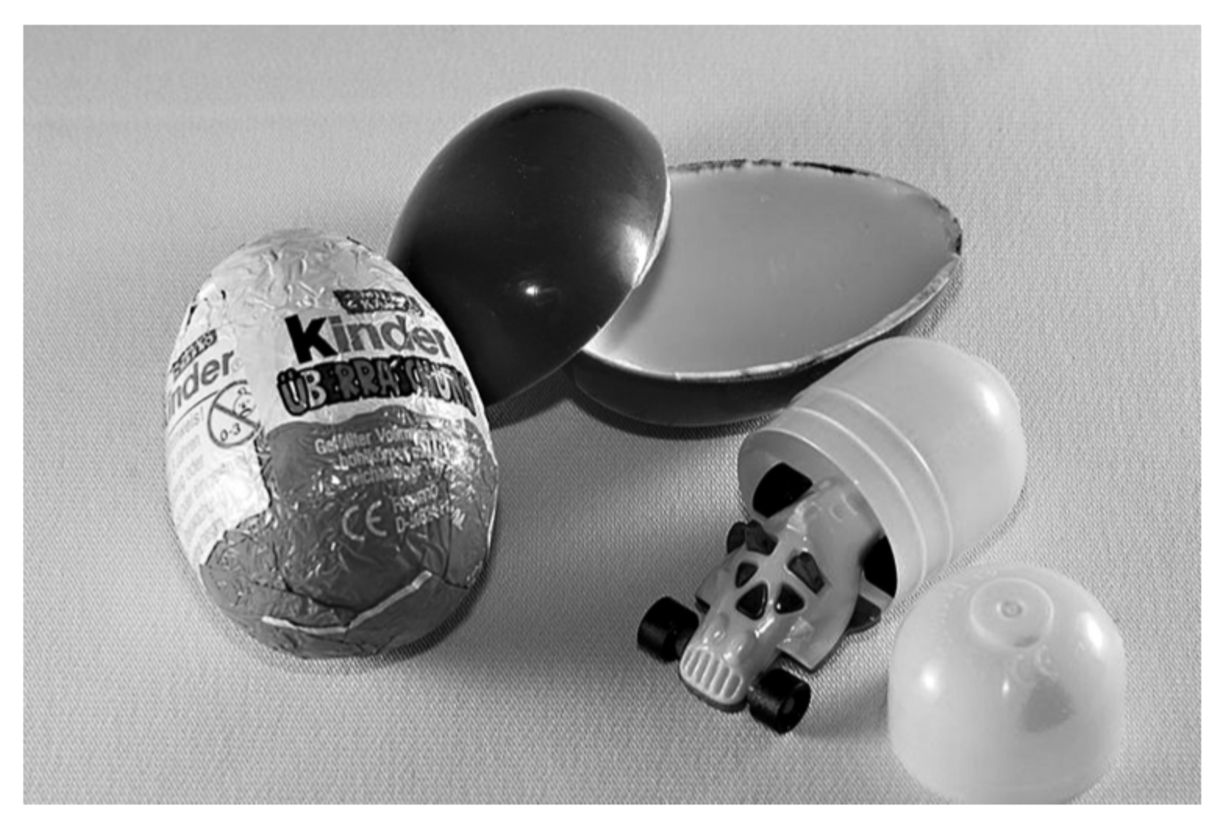
\includegraphics{../_database/Bilder/Bild57-1.eps}}
\end{center}
\begin{scriptsize}\begin{singlespace}Bildquelle: https://de.wikipedia.org/wiki/Datei:Überraschungsei.jpg [01.06.2015] (Urheber: A. Kniesel, Lizenz: CC BY-SA 3.0)\end{singlespace}\end{scriptsize}

\subsection{Aufgabenstellung:}
\begin{enumerate}
	\item Bei der Qualitätskontrolle gelten Schokoladeneier, deren Masse um mehr als 0,5\,g vom Sollwert 20\,g abweichen, als Ausschuss. Bei einer Kontrolle wurden nach dem Zufallsprinzip 500 Schokoladeneier einer Produktionsserie ausgewählt und überprüft. Dabei wurden 15 als Ausschuss aussortiert.\leer
	
 Gib ein symmetrisches 90-\%-Konfidenzintervall für den relativen Anteil $p$ an Ausschusseiern in der gesamten Produktionsserie an!\leer

 Gib an, durch welche Maßnahme man die Breite des Konfidenzintervalls bei vorgegebenem Konfidenzniveau (Sicherheit) verringern kann!\leer

\item Der Hersteller überlegt, die gelbe Kapsel in Zukunft nur in Form eines Drehzylinders ohne aufgesetzte Halbkugeln zu produzieren. Das Volumen $V$ der Kapsel soll dabei unverändert bleiben, ebenso wie die Form des Schokoladeneies. Die Oberfläche $O(r)$ des angedachten Drehzylinders kann in Abhängigkeit vom Radius $r$ durch die Funktion $O$ mit der Gleichung $O(r)=2r^2\pi+2\cdot V\cdot r^{-1}$ beschrieben werden. Der Radius $r$ darf dabei nur Werte im Bereich $(0\,cm; 1,9\,cm]$ annehmen, damit der Zylinder in das Schokoladenei passt.\leer

 Berechne die minimal mögliche Oberfläche der geplanten zylindrischen Kapsel!\leer

 Weise durch Differenzialrechnung nach, dass an der berechneten Stelle tatsächlich ein Minimum vorliegt!
						\end{enumerate}\leer
				
\antwort{
\begin{enumerate}
	\item \subsection{Lösungserwartung:} 
	
$h=0,03$

$0,03\,\pm\,1,645\cdot\sqrt{\frac{0,03\cdot(1-0,03)}{500}} \approx 0,03\,\pm\,0,013 \Rightarrow [0,017;0,043]$\leer

Mögliche Maßnahme:

Durch eine Erhöhung der Anzahl der kontrollierten Schokoladeneier auf mehr als 500 kann eine Verringerung der Breite des Konfidenzintervalls erreicht werden.
		
	\subsection{Lösungsschlüssel:}
	\begin{itemize}
		\item Ein Punkt für ein korrektes Intervall. Andere Schreibweisen des Ergebnisses (als Bruch oder Dezimalzahl) sind ebenfalls als richtig zu werten. 
		
		Toleranzintervall für den unteren Wert: $[0,017; 0,02]$ 
		
		Toleranzintervall für den oberen Wert: $[0,042; 0,05]$ 
		
		Die Aufgabe ist auch dann als richtig gelöst zu werten, wenn bei korrektem Ansatz das Ergebnis aufgrund eines Rechenfehlers nicht richtig ist. 
		\item Ein Punkt für eine (sinngemäß) korrekte Angabe der entsprechenden Änderung. Andere angeführte korrekte Maßnahmen sind ebenfalls als richtig zu werten.
	\end{itemize}
	
	\item \subsection{Lösungserwartung:}
			
			$O'(r)=4r\pi-72\cdot r^{-2}=4r\pi-\frac{72}{r^2}$
	
	$4r\pi-\frac{72}{r^2}=0$
	
	$r^3=\frac{18}{\pi}$
	
	$r=\sqrt[3]{\frac{18}{\pi}} \Rightarrow r\approx 1,79$\,cm
	
	$O(1,79)\approx 60,4$\,cm$^2$
	
	$O''(r)=4\pi+144\cdot r^{-3}=4\pi+\frac{144}{r^3}$
	
	$O''(1,79)\approx 37,7>0$, daher liegt ein lokales Maximum vor.

	\subsection{Lösungsschlüssel:}
	
\begin{itemize}
	\item    Ein Punkt für eine korrekte Berechnung der minimalen Oberfläche, wobei die Einheit "`cm$^2$"' nicht angeführt sein muss. 
	
	Toleranzintervall: $[60\,\text{cm}^2; 61\,\text{cm}^2] $ 
	
	Die Aufgabe ist auch dann als richtig gelöst zu werten, wenn bei korrektem Ansatz das Ergebnis aufgrund eines Rechenfehlers nicht richtig ist. 
	\item  Ein Punkt für einen korrekten Nachweis. Andere angeführte korrekte Nachweise sind ebenfalls als richtig zu werten. 
\end{itemize}

\end{enumerate}}
		\end{langesbeispiel}%
\hrule  \leer

\section{61 - MAT - WS 3.1, WS 3.2, WS 3.4,  - Würfel mit unterschiedlichen Zahlen - Matura 2015/16 Haupttermin}

\begin{langesbeispiel} \item[0] %PUNKTE DES BEISPIELS
	
 Gegeben sind die Netze von drei fairen Würfeln, deren Seitenflächen auf unterschiedliche Weise mit verschiedenen Zahlen beschriftet sind. (Ein Würfel ist "`fair"', wenn die Wahrscheinlichkeit, nach einem Wurf nach oben zu zeigen, für alle Seitenflächen gleich groß ist.)

\begin{center}
	\resizebox{0.9\linewidth}{!}{\psset{xunit=1.0cm,yunit=1.0cm,algebraic=true,dimen=middle,dotstyle=o,dotsize=4pt 0,linewidth=0.8pt,arrowsize=3pt 2,arrowinset=0.25}
\begin{pspicture*}(0.17804133915570747,4.040102465944372)(15.692206630376225,9.148214730906863)
\psline[linewidth=0.8pt](1.,7.)(1.,6.)
\psline[linewidth=0.8pt](1.,6.)(2.,6.)
\psline[linewidth=0.8pt](2.,6.)(2.,7.)
\psline[linewidth=0.8pt](2.,7.)(1.,7.)
\psline[linewidth=0.8pt](2.,6.)(3.,6.)
\psline[linewidth=0.8pt](3.,6.)(3.,5.)
\psline[linewidth=0.8pt](3.,5.)(4.,5.)
\psline[linewidth=0.8pt](4.,5.)(4.,6.)
\psline[linewidth=0.8pt](4.,6.)(5.,6.)
\psline[linewidth=0.8pt](5.,6.)(5.,7.)
\psline[linewidth=0.8pt](5.,7.)(4.,7.)
\psline[linewidth=0.8pt](4.,7.)(4.,8.)
\psline[linewidth=0.8pt](4.,8.)(3.,8.)
\psline[linewidth=0.8pt](3.,8.)(3.,7.)
\psline[linewidth=0.8pt](3.,7.)(2.,7.)
\psline[linewidth=0.8pt](3.,7.)(3.,6.)
\psline[linewidth=0.8pt](3.,7.)(4.,7.)
\psline[linewidth=0.8pt](3.,6.)(4.,6.)
\psline[linewidth=0.8pt](4.,7.)(4.,6.)
\psline[linewidth=0.8pt](5.94,6.97)(5.94,5.97)
\psline[linewidth=0.8pt](5.94,5.97)(6.94,5.97)
\psline[linewidth=0.8pt](6.94,5.97)(6.94,6.97)
\psline[linewidth=0.8pt](6.94,6.97)(5.94,6.97)
\psline[linewidth=0.8pt](6.94,5.97)(7.94,5.97)
\psline[linewidth=0.8pt](7.94,5.97)(7.94,4.97)
\psline[linewidth=0.8pt](7.94,4.97)(8.94,4.97)
\psline[linewidth=0.8pt](8.94,4.97)(8.94,5.97)
\psline[linewidth=0.8pt](8.94,5.97)(9.94,5.97)
\psline[linewidth=0.8pt](9.94,5.97)(9.94,6.97)
\psline[linewidth=0.8pt](9.94,6.97)(8.94,6.97)
\psline[linewidth=0.8pt](8.94,6.97)(8.94,7.97)
\psline[linewidth=0.8pt](8.94,7.97)(7.94,7.97)
\psline[linewidth=0.8pt](7.94,7.97)(7.94,6.97)
\psline[linewidth=0.8pt](7.94,6.97)(6.94,6.97)
\psline[linewidth=0.8pt](7.94,6.97)(7.94,5.97)
\psline[linewidth=0.8pt](7.94,6.97)(8.94,6.97)
\psline[linewidth=0.8pt](7.94,5.97)(8.94,5.97)
\psline[linewidth=0.8pt](8.94,6.97)(8.94,5.97)
\psline[linewidth=0.8pt](10.96,6.95)(10.96,5.95)
\psline[linewidth=0.8pt](10.96,5.95)(11.96,5.95)
\psline[linewidth=0.8pt](11.96,5.95)(11.96,6.95)
\psline[linewidth=0.8pt](11.96,6.95)(10.96,6.95)
\psline[linewidth=0.8pt](11.96,5.95)(12.96,5.95)
\psline[linewidth=0.8pt](12.96,5.95)(12.96,4.95)
\psline[linewidth=0.8pt](12.96,4.95)(13.96,4.95)
\psline[linewidth=0.8pt](13.96,4.95)(13.96,5.95)
\psline[linewidth=0.8pt](13.96,5.95)(14.96,5.95)
\psline[linewidth=0.8pt](14.96,5.95)(14.96,6.95)
\psline[linewidth=0.8pt](14.96,6.95)(13.96,6.95)
\psline[linewidth=0.8pt](13.96,6.95)(13.96,7.95)
\psline[linewidth=0.8pt](13.96,7.95)(12.96,7.95)
\psline[linewidth=0.8pt](12.96,7.95)(12.96,6.95)
\psline[linewidth=0.8pt](12.96,6.95)(11.96,6.95)
\psline[linewidth=0.8pt](12.96,6.95)(12.96,5.95)
\psline[linewidth=0.8pt](12.96,6.95)(13.96,6.95)
\psline[linewidth=0.8pt](12.96,5.95)(13.96,5.95)
\psline[linewidth=0.8pt](13.96,6.95)(13.96,5.95)
\rput[tl](1.4,6.6){1}
\rput[tl](2.4,6.6){2}
\rput[tl](3.4,6.6){1}
\rput[tl](4.4,6.6){2}
\rput[tl](3.4,7.6){3}
\rput[tl](3.4,5.6){3}
\rput[tl](6.3,6.6){-1}
\rput[tl](7.35,6.6){2}
\rput[tl](8.3,6.6){-1}
\rput[tl](9.35,6.6){2}
\rput[tl](8.35,7.6){5}
\rput[tl](8.35,5.6){5}
\rput[tl](11.4,6.6){0}
\rput[tl](12.4,6.6){0}
\rput[tl](13.4,6.6){6}
\rput[tl](13.4,5.6){6}
\rput[tl](13.4,7.6){0}
\rput[tl](14.4,6.6){6}
\rput[tl](2.6,8.665014922059061){Würfel $A$}
\rput[tl](7.6,8.665014922059061){Würfel $B$}
\rput[tl](12.6,8.665014922059061){Würfel $C$}
\end{pspicture*}}
\end{center}



\subsection{Aufgabenstellung:}
\begin{enumerate}
	\item Herr Fischer wirft Würfel $A$ zweimal. Die Zufallsvariable $X$ gibt die Summe der beiden geworfenen Zahlen an. Die Zufallsvariable $X$ kann die Werte 2,3,4,5 und 6 annehmen.
	
	Frau Fischer wirft die Würfel $A$ und $B$. Die Zufallsvariable $Y$ gibt die Summe der beiden geworfenen Zahlen an.\leer
	
	\fbox{A} Gib für die Zufallsvariable $Y$ alle möglichen Werte an!
	
	mögliche Wert für $Y$: \rule{5cm}{0.3pt}
	
	Es gibt Werte der Zufallsvariablen, die bei Herrn Fischer wahrscheinlicher auftreten als bei Frau Fischer. Gib denjenigen Wert an, bei dem der Unterschied der beiden Wahrscheinlichkeiten am größten ist, und berechne diesen Unterschied!
	
	\item Bei einem Spiel wird Würfel $B$ dreimal geworfen. Der Einsatz des Spiels für eine Spielerin/einen Spieler beträgt \EUR{2}. Die jeweilige Auszahlung ist von der Summe der drei geworfenen Zahlen abhängig und wird in der nachstehenden Tabelle teilweise angegeben
	
	\begin{center}
		\begin{tabular}{|c|c|}\hline
		\cellcolor[gray]{0.9}Summe der drei geworfenen Zahlen&\cellcolor[gray]{0.9}Auszahlung an die Spielerin/den Spieler\\ \hline
		positiv&0\\ \hline
		null&2\\ \hline
		negativ&?\\ \hline		
		\end{tabular}
	\end{center}

Eine Person spielt dieses Spiel fünfmal. Berechne die Wahrscheinlichkeit, dass dabei genau zweimal die Summe der drei geworfenen Zahlen genau null ist!

 Berechne, welchen Betrag der Anbieter des Spiels für das Würfeln einer negativen Summe höchstens auszahlen darf, um langfristig mit keinem Verlust rechnen zu müssen! 

\item  Peter wirft den Würfel $C$ 100-mal. Die Zufallsvariable $Z$ beschreibt die Anzahl der gewürfelten Sechser.

 Berechne den Erwartungswert und die Standardabweichung von $Z$!

 Ermittle die Wahrscheinlichkeit, dass die Summe der geworfenen Zahlen größer als 350 ist!    
						\end{enumerate}\leer
				
\antwort{
\begin{enumerate}
	\item \subsection{Lösungserwartung:} 
	
mögliche Werte für $Y$: $0, 1, 2, 3, 4, 5, 6, 7, 8$

Bei $Y$ hat jeder Wert die gleiche Wahrscheinlichkeit $\left(=\frac{1}{9}\right)$, bei $X$ hat 4 die größte Wahrscheinlichkeit $\left(=3\cdot\frac{1}{3}\cdot\frac{1}{3}=\frac{1}{3}\right)$. Der Unterschied ist bei 4 am größten, er beträgt $\frac{2}{9}$.

oder:

Die Wahrscheinlichkeit für 4 ist bei Herrn Fischer dreimal so groß wie bei Frau Fischer.

	\subsection{Lösungsschlüssel:}
	\begin{itemize}
		\item Ein Ausgleichspunkt für die vollständige Angabe der korrekten Werte für $Y$. 
		\item Ein Punkt für die Angabe des gesuchten Wertes und einer korrekten Berechnung des Unterschieds.
	\end{itemize}
	
	\item \subsection{Lösungserwartung:}
			
	Mögliche Berechnung:
	
	Zufallsvariable $X$ = Anzahl der Spiele, bei denen die Summe der drei geworfenen Zahlen genau null ist.
	
	$P(\text{"`Summe der drei geworfenen Zahlen ist null"'})=p=\frac{1}{3}\cdot\frac{1}{3}\cdot\frac{1}{3}\cdot 3=\frac{1}{9}$
	
	Binomialverteilung mit den Parametern $n=5, k=2, p=\frac{1}{9}$
	
	$P(X=2)=\binom{5}{2}\cdot\left(\frac{1}{9}\right)²\cdot\left(\frac{8}{9}\right)³\approx 0,087 \Rightarrow$ Die gesuchte Wahrscheinlichkeit liegt bei ca. 8,7\,\%.
	
	Mögliche Berechnung:
	
	$x$ ... Auszahlung für das Würfeln einer negativen Summe
	
	$2\cdot\frac{1}{9}+x\cdot\frac{1}{27}<2 \Rightarrow x<48$
	
	Die Auszahlung für das Würfeln einer negativen Summe darf höchstens \EUR{48} betragen, damit der Anbieter des Spiels langfristig mit keinem Verlust rechnen muss.

	\subsection{Lösungsschlüssel:}
	
\begin{itemize}
	\item   Ein Punkt für die richtige Lösung. Andere Schreibweisen des Ergebnisses sind ebenfalls als richtig zu werten. 
	
	Toleranzintervall: $[0,08; 0,09]$ bzw. $[8\,\%; 9\,\%]$
	\item  Ein Punkt für die richtige Lösung, wobei die Einheit "`\EUR{ }"' nicht angegeben sein muss. Die Aufgabe ist auch dann als richtig gelöst zu werten, wenn bei korrektem Ansatz das Ergebnis aufgrund eines Rechenfehlers nicht richtig ist.

\end{itemize}

\item \subsection{Lösungserwartung:}
			
$n=100$ und $p=0,5$\leer

Erwartungswert: $E(Z)=50$

Standardabweichung: $\sqrt{V(Z)}=5$

Mögliche Berechnung (z.B. durch Approximation durch die Normalverteilung ohne Stetigkeitskorrektur):  

Die Summe ist größer als 350, wenn die Anzahl der Sechser mindestens 59 ist. Es ist möglich, die (für die Anzahl der Sechser) zugrunde liegende Binomialverteilung mit $n=100$ und $p=0,5$ durch die Normalverteilung mit $\mu=50$ und $\sigma=5$ zu approximieren.

$P(Z\geq 59)\approx 0,036=36\,\%$

	\subsection{Lösungsschlüssel:}
	
\begin{itemize}
	\item Ein Punkt für die Angabe der beiden korrekten Werte für den Erwartungswert und die Standardabweichung.
	\item Ein Punkt für die richtige Lösung, wobei Ergebnisse durch Berechnung mit Stetigkeitskorrektur oder exakt mittels Binomialverteilung ebenfalls als richtig zu werten sind. 
	
	Die Aufgabe ist auch dann als richtig gelöst zu werten, wenn bei korrektem Ansatz das Ergebnis aufgrund eines Rechenfehlers nicht richtig ist. 
	
	Toleranzintervall: $[0,035; 0,045]$ bzw. $[3,5\,\%; 4,5\,\%]$
\end{itemize}

\end{enumerate}}
		\end{langesbeispiel}%
\hrule  \leer

\section{64 - MAT - AG 4.1, AG 3.3, AG 3.4, WS 4.1 - Pong - Matura 2015/16 1. Nebentermin}

\begin{langesbeispiel} \item[0] %PUNKTE DES BEISPIELS
	
Das 1972 vom Unternehmen Atari veröffentlichte \textit{Pong} wurde zum ersten weltweit populären Videospiel. (Quelle: http://de.wikipedia.org/wiki/Pong)

Das Spielprinzip von \textit{Pong} ist wie folgt: Ein Punkt ("`Ball"') bewegt sich auf dem Bildschirm entlang geradliniger Bahnen hin und her. Jede/r der beiden Spieler/innen steuert einen senkrechten Strich ("`Schläger"'), den sie/er mit einem Drehknopf ("`Joystick"') nach oben und unten verschieben kann. 

Lässt man den Ball am Schläger vorbei, erhält die Gegnerin / der Gegner einen Punkt.

Das Spielfeld, in dem sich der Ball und die Schläger bewegen, hat eine Breite von 800 Pixeln und eine Höhe von 600 Pixeln (ein Pixel ist ein quadratischer Bildpunkt). Vereinfachend wird angenommen, dass der Ball als Pixel dargestellt wird. 

Wenn der Ball den oberen bzw. unteren Spielfeldrand oder einen Schläger berührt, dann wird er von dort reflektiert. Dabei gilt das Reflexionsgesetz; dieses besagt: $\alpha=\beta$ (vgl. die unten abgebildete Grafik).

Man kann sich das Spielfeld als Ebene mit Koordinatensystem vorstellen. Der Bildpunkt $(1|1)$ liegt dann in der linken unteren Ecke, der Bildpunkt $(800|600)$ in der rechten oberen Ecke.

Auf dem Schirm wird das Bild alle 0,02 Sekunden neu generiert. Der Geschwindigkeitsvektor $\vec{v}=\binom{v_x}{v_y}$ das Balls gibt an, um wie viele Pixel sich der Ball von einem Bildaufbau zum nächsten in horizontaler Richtung $\left(v_x\right)$ und in vertikaler Richtung $\left(v_y\right)$ weiterbewegt hat.

\begin{center}
	\resizebox{0.5\linewidth}{!}{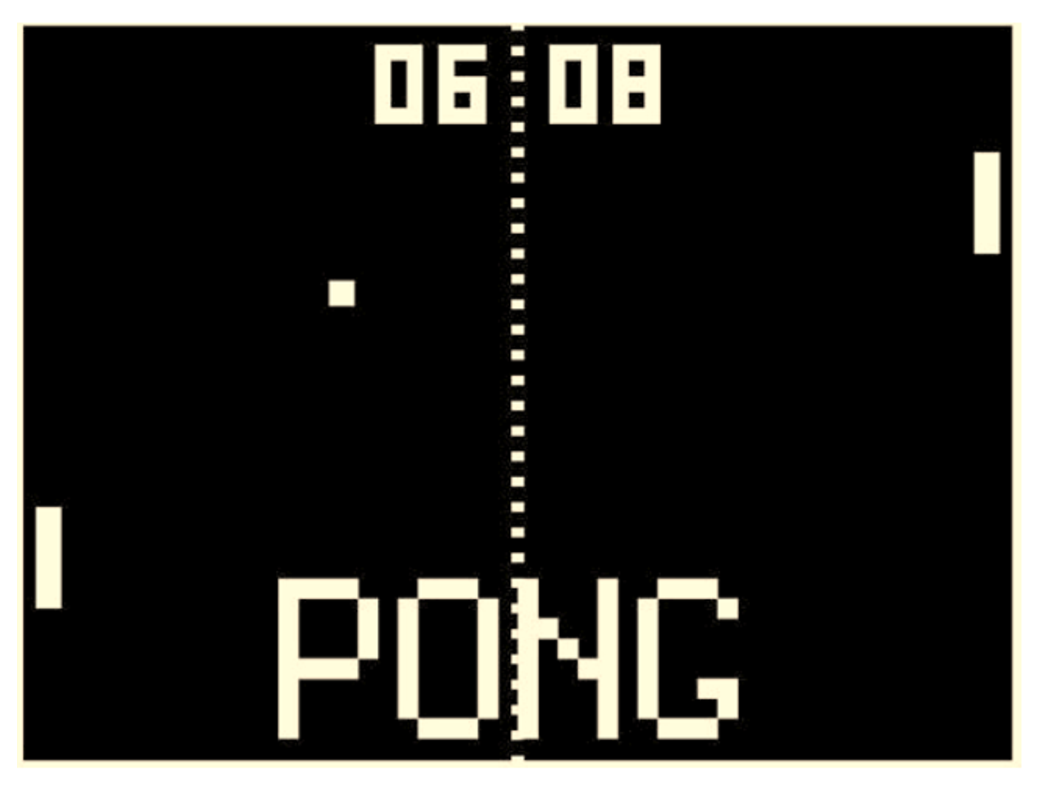
\includegraphics{../Bilder/Bild64-1.eps}}
\end{center}
\begin{scriptsize} Bildquelle: http://www.overclockers.at/games\_forum/euer-erstes-computerspiel\_237146/page\_2 [15.10.2015]. \end{scriptsize}

\begin{center}
	\resizebox{0.5\linewidth}{!}{\newrgbcolor{qqwuqq}{0. 0.39215686274509803 0.}
\psset{xunit=1.0cm,yunit=1.0cm,algebraic=true,dimen=middle,dotstyle=o,dotsize=4pt 0,linewidth=0.8pt,arrowsize=3pt 2,arrowinset=0.25}
\begin{pspicture*}(0.66,5.447272727272732)(8.9,8.537922077922087)
\multips(0,5)(0,1.0){4}{\psline[linestyle=dashed,linecap=1,dash=1.5pt 1.5pt,linewidth=0.4pt,linecolor=lightgray]{c-c}(0.66,0)(8.9,0)}
\multips(0,0)(1.0,0){9}{\psline[linestyle=dashed,linecap=1,dash=1.5pt 1.5pt,linewidth=0.4pt,linecolor=lightgray]{c-c}(0,5.447272727272732)(0,8.537922077922087)}
\psaxes[labelFontSize=\scriptstyle,xAxis=true,yAxis=true,Dx=1.,Dy=1.,ticksize=-2pt 0,subticks=2]{->}(0,0)(0.66,5.447272727272732)(8.9,8.537922077922087)
\psplot[linewidth=0.8pt]{0.66}{8.9}{(--56.-0.*x)/7.}
\psline[linewidth=0.8pt]{->}(5.,8.)(8.,6.)
\psline[linewidth=0.8pt]{->}(2.,6.)(5.,8.)
\pscustom[linewidth=0.8pt,linecolor=qqwuqq,fillcolor=qqwuqq,fillstyle=solid,opacity=0.1]{
\parametricplot{-0.5880026035475675}{0.0}{1.4*cos(t)+5.|1.4*sin(t)+8.}
\lineto(5.,8.)\closepath}
\pscustom[linewidth=0.8pt,linecolor=qqwuqq,fillcolor=qqwuqq,fillstyle=solid,opacity=0.1]{
\parametricplot{3.141592653589793}{3.7295952571373605}{1.4*cos(t)+5.|1.4*sin(t)+8.}
\lineto(5.,8.)\closepath}
\rput[bl](5.8,7.5){\qqwuqq{$\beta$}}
\rput[bl](3.9,7.58){\qqwuqq{$\alpha$}}
\end{pspicture*}}
\end{center}

\subsection{Aufgabenstellung:}
\begin{enumerate}
	\item In einer konkreten Spielsituation hat der Ball beim Aufprall auf den oberen Spielfeldrand einen Geschwindigkeitsvektor von $\vec{v}=\binom{4}{7}$ Pixeln pro Bildaufbau.
	
	\fbox{A} Gib denjenigen Winkel $\alpha$ an, unter dem der Ball auf den Spielfeldrand trifft!
	
	$\alpha$= \rule{5cm}{0.3pt}
	
	Die Komponenten des Geschwindigkeitsvektors sind immer ganzzahlig. Nehmen Sie an, dass die Summe der Beträge der Komponenten nicht größer als 20 sein darf.
	
	Der Ball wird am oberen Spielfeldrand unter dem Winkel $\beta$ reflektiert. Welchen kleinstmöglichen Wert $\beta_\text{min}$ kann unter diesen Voraussetzungen der Winkel $\beta$ annehmen? Gib $\beta_\text{min}$ an!
	
	$\beta_\text{min}$= \rule{5cm}{0.3pt}
	
	\item In einem anderen Spielverlauf befindet sich der Ball im Punkt $(401|301)$ und sein Geschwindigkeitsvektor ist dabei $\vec{v}=\binom{2}{-3}$ Pixel pro Bildaufbau.
	
	Gib an, wie viele \textit{Sekunden} es dauert, bis der Ball am unteren Spielfeldrand reflektiert wird.
	
	Nach dieser Reflexion bewegt sich der Ball entlang einer Geraden bis zum nächsten Auftreffen auf den Schläger oder den Spielfeldrand.
	
 Gib eine Parameterdarstellung dieser Geraden an! 

\item Zwei Kinder, Nicola und Florian, spielen über einen längeren Zeitraum oft gegeneinander \textit{Pong}. Von 45 Spielen gewinnt Nicola 31-mal, Florian gewinnt 14-mal.
 
		Gib auf Basis dieser Information ein symmetrisches $95-\%-$Konfidenzintervall für Nicolas Gewinnwahrscheinlichkeit an!
		
		Erkläre, wieso es nicht sinnvoll ist, ein 100-\%-Konfidenzintervall zu bestimmen!
\end{enumerate}
\antwort{
\begin{enumerate}
	\item \subsection{Lösungserwartung:} 
	
$\tan(\alpha)=\frac{7}{4}=1,74$

$\alpha\approx 60,26^\circ$

Unter diesen Bedingungen lautet der Geschwindigkeitsvektor $\vec{v}= \binom{\pm\,19}{\pm\,1}$ Pixel pro Bildaufbau. Für den Winkel $\beta_\text{min}$ gibt das in jedem Fall:

 $\tan(\beta_\text{min})=\frac{1}{19}$

 $\beta_\text{min}\approx 3,01^\circ$

	\subsection{Lösungsschlüssel:}
	\begin{itemize}
		\item Ein Ausgleichspunkt für die richtige Lösung, wobei die Einheit "`Grad"' nicht angegeben sein muss. Eine korrekte Angabe der Lösung in einer anderen Einheit ist ebenfalls als richtig zu werten. 
		
		Toleranzintervall: $[6011^\circ; 60,3^\circ]$
		\item Ein Punkt für die richtige Lösung, wobei die Einheit "`Grad"' nicht angegeben sein muss. Eine korrekte Angabe der Lösung in einer anderen Einheit ist ebenfalls als richtig zu werten. 
		
		Toleranzintervall: $[3^\circ; 3,02^\circ]$
	\end{itemize}
	
	\item \subsection{Lösungserwartung:}
			
	$301-3n=1 \Rightarrow n=100$
	
	$100\cdot 0,02=2$
	
	Es dauert zwei Sekunden, bis der Ball am unteren Spielfeldrand reflektiert wird.\leer
	
	$g: X=\binom{601}{1}+s\cdot\binom{2}{3}$

	\subsection{Lösungsschlüssel:}
	
\begin{itemize}
	\item Ein Punkt für die richtige Lösung. 
	
	Toleranzintervall: $[2\,\text{s}; 2,02\,\text{s}]$
	\item Ein Punkt für eine korrekte Parameterdarstellung bzw. Gleichung der Geraden. Äquivalente Parameterdarstellungen bzw. Gleichungen sind als richtig zu werten. 
\end{itemize}

\item \subsection{Lösungserwartung:}
			
$n=45, h=\frac{31}{45}$

$\frac{31}{45}\,\pm\,1,96\cdot\sqrt{\frac{\frac{31}{45}\cdot\frac{14}{45}}{45}}\approx 0,689\,\pm\,0,135 \Rightarrow [0,554;0,824]$\leer

Mögliche Erklärungen:

Es ist nicht sinnvoll, ein 100-\%-Konfidenzintervall zu bilden, da die Intervallgrenzen dann 0\,\% bis 100\.\% wären, man hätte also keinen Informationsgewinn. 

 oder:  

 Ein 100-\%-Konfidenzintervall erstreckt sich über den gesamten Definitionsbereich.
	\subsection{Lösungsschlüssel:}
	
\begin{itemize}
	\item Ein Punkt für ein korrektes Intervall. Andere Schreibweisen des Ergebnisses (als Bruch oder in Prozent) sind ebenfalls als richtig zu werten. 
	
	Toleranzintervall für den unteren Wert: $[0,54; 0,56]$ 
	
	Toleranzintervall für den oberen Wert: $[0,81; 0,83]$ 
	
	Die Aufgabe ist auch dann als richtig gelöst zu werten, wenn bei korrektem Ansatz das Ergebnis aufgrund eines Rechenfehlers nicht richtig ist. 
	\item Ein Punkt für eine (sinngemäß) korrekte Erklärung.
\end{itemize}
\end{enumerate}}
		\end{langesbeispiel}%
\hrule  \leer

\section{65 - MAT - WS 2.1, WS 3.4, WS 2.3 - Roulette - Matura 2015/16 1. Nebentermin}

\begin{langesbeispiel} \item[0] %PUNKTE DES BEISPIELS
	
Beim Glücksspiel \textit{Roulette} versucht man, diejenige Zahl bzw. Gruppe von Zahlen zu erraten, die durch den Wurf einer Kugel in die Roulettemaschine bestimmt wird. 

Beim \textit{französischen Roulette} besteht die Roulettemaschine aus einer in eine Schüssel eingelassenen, drehbaren Scheibe mit 36 abwechselnd roten und schwarzen Nummernfächern sowie einem 37., grün gekennzeichneten Fach für die Null (vgl. Abbildung 1). Die Roulettescheibe wird in Bewegung gesetzt und die Kugel wird gegen die Drehrichtung in die Roulettemaschine geworfen. Dabei wird kein Nummernfach bevorzugt und es gibt keine Möglichkeit, das Ergebnis (etwa durch "`geschicktes"' Werfen) zu beeinflussen. 

Ziel ist es, in jedem einzelnen Spiel im Vorhinein zu erraten, in welchem Nummernfach die Kugel zu liegen kommen wird. 

Auf dem Spielfeld (vgl. Abbildung 2) werden die Spieleinsätze (Jetons) platziert. Beispielsweise sind die Felder mit der "`1"' und der "`7"' rot ("`rouge"'), die Felder mit der "`4"' und der "`6"' schwarz ("`noir"').

\meinlr{\resizebox{1\linewidth}{!}{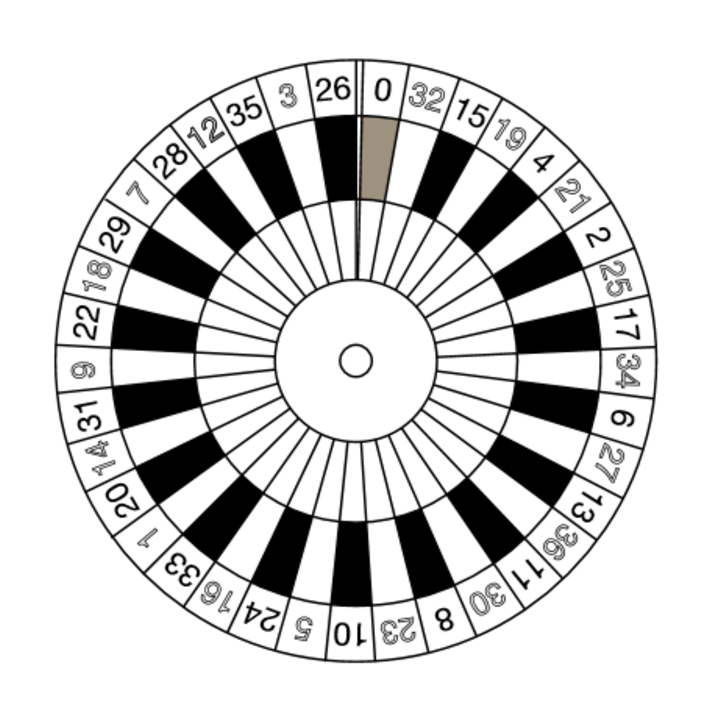
\includegraphics{../_database/Bilder/Bild65-1.eps}}

Abbildung 1

\begin{scriptsize}\begin{singlespace}Quelle:http://www.rouletteplay.com/images/\\
software\_logos\_small/european-roulette-wheel.gif [23.03.2016]\end{singlespace}\end{scriptsize}}{\resizebox{0.8\linewidth}{!}{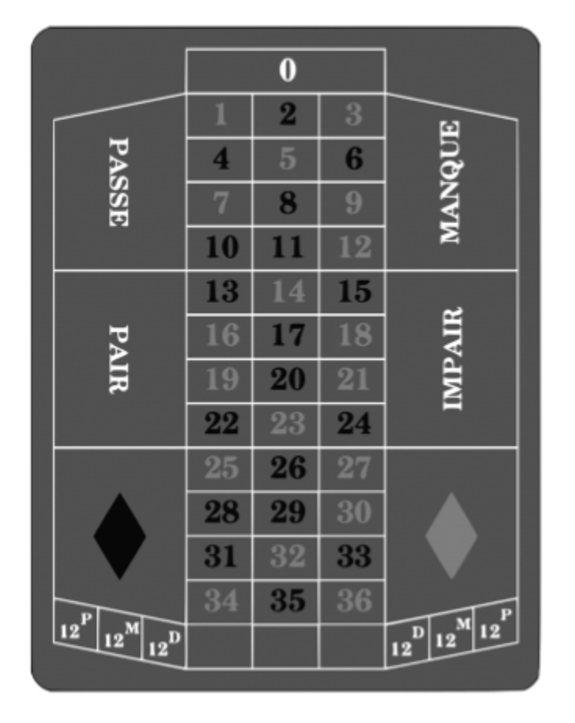
\includegraphics{../_database/Bilder/Bild65-2.eps}}

Abbildung 2

\begin{scriptsize}\begin{singlespace}Quelle:http://commons.wikimedia.org/wiki/\\
File:Roulette\_frz.png [23.03.2016]\end{singlespace}\end{scriptsize}}
 

\subsection{Aufgabenstellung:}
\begin{enumerate}
	\item Jemand argumentiert: "`Wenn die Kugel bei fünf Spielen hintereinander jedes Mal auf ein rotes Feld gefallen ist, fällt die Kugel beim 6. Spiel mit höherer Wahrscheinlichkeit auf ein schwarzes Feld als auf ein rotes, da bei einer längeren Spielserie dieselben Häufigkeiten für 'Rouge' und 'Noir' zu erwarten sind."' Gib an, ob diese Argumentation richtig oder falsch ist, und begründe deine Entscheidung!\leer
	
	An einem Roulettetisch werden an einem Abend 100 Spiele gespielt.
	
	\fbox{A} Berechne die Wahrscheinlichkeit, dass die Kugel dabei höchstens 40-mal in ein rotes Nummernfach fällt!\leer
	
	\item In der folgenden Tabelle sind einige Wettmöglichkeiten sowie die jeweiligen Gewinnquoten angeführt:\leer
	
	\begin{tabular}{|l|c|}\hline
	\cellcolor[gray]{0.9}Wettart&\cellcolor[gray]{0.9}Gewinnquote\\ \hline
	Rouge: Die Kugel fällt in ein rotes Nummernfach.&1:1\\ \hline
	Noir: Die Kugel fällt in ein schwarzes Nummernfach.&1:1\\ \hline
	$12^\text{P}$: erstes Dutzend (Zahlen 1 bis 12)&2:1\\ \hline
	$12^\text{M}$: mittleres Dutzend (Zahlen 13 bis 24)&2:1\\ \hline
	$12^\text{D}$: letztes Dutzend (Zahlen 25 bis 36)&2:1\\ \hline
	Plein: Man setzt auf eine der 37 Zahlen&35:1\\ \hline
	\multicolumn{1}{|p{10cm}|}{Cheval: Man setzt auf zwei auf dem Spielfeld horizontal oder vertikal benachbarte Zahlen, z.B. 2 und 5 oder 8 und 9.}&17:1\\ \hline	
	\end{tabular}\leer
	
 Eine Gewinnquote von $2:1$ bedeutet beispielsweise, dass im Falle eines Gewinns der Einsatz und zusätzlich das Doppelte des Einsatzes ausbezahlt wird. Im Falle eines Verlustes verliert man den Einsatz.

 Als Bankvorteil bezeichnet man bei Glücksspielen den erwarteten Verlust der Spielerin/des Spielers bezogen auf ihren/seinen Einsatz.

Eine Spielerin setzt \EUR{10} auf $12^\text{M}$. 

Berechne den Bankvorteil in Prozent des Einsatzes! 
 
Gib an, ob der in Prozent angegebene Bankvorteil größer wird, kleiner wird oder gleich bleibt, wenn die Spielerin/der Spieler bei einem Einsatz von \EUR{$a$} eine Cheval-Variante wählt!  

Begründe deine Entscheidung!


	
\end{enumerate}
\antwort{
\begin{enumerate}
	\item \subsection{Lösungserwartung:} 
	
Die Argumentation ist falsch. Da die einzelnen Spiele unabhängig voneinander sind, gilt auch für das sechste Spiel (unabhängig von den vorherigen Spielausgängen):

$P(\text{"`Rouge"'})=P(\text{"`Noir"'})=\frac{18}{37}$\leer

Mögliche Berechnung (z.B. durch Approximation durch die Normalverteilung ohne Stetigkeitskorrektur):  

Die binomialverteilte Zufallsvariable $X$ beschreibt, wie oft die Kugel in ein rotes Nummernfach fällt.

$n=100, p=\frac{18}{37}$

$P(X\leq 40)\approx 0,0418$ 

	\subsection{Lösungsschlüssel:}
	\begin{itemize}
		\item  Ein Punkt für die Angabe, dass die Argumentation nicht richtig ist, und für eine (sinngemäß) korrekte Begründung.
		\item  Ein Ausgleichspunkt für die richtige Lösung, wobei Ergebnisse durch Berechnung mit Stetigkeitskorrektur oder exakt mittels Binomialverteilung ebenfalls als richtig zu werten sind. Andere Schreibweisen des Ergebnisses (in Prozent) sind ebenfalls als richtig zu werten. 
		
		Toleranzintervall: $[0,03; 0,06]$  
		
		Die Aufgabe ist auch dann als richtig gelöst zu werten, wenn bei korrektem Ansatz das Ergebnis aufgrund eines Rechenfehlers nicht richtig ist. 
	\end{itemize}
	
	\item \subsection{Lösungserwartung:}
			
	Mögliche Berechnung:
	
	Bei $12^\text{M}$ erhält die Spielerin bei einem Einsatz von \EUR{10} mit der Wahrscheinlichkeit $\frac{12}{37}$ einen Gewinn von \EUR{20}.
	
	$\frac{12}{37}\cdot 20-\frac{25}{37}\cdot 10\approx -0,27$
	
	D.h., der erwartete Verlust beträgt ca. \EUR{0,27}.
	
	Bankvorteil: \EUR{0,27} bzw. 2,7\,\% des Einsatzes\leer
	
	Cheval bei einem Einsatz von \EUR{$a$}:
	
	erwarteter Gewinn: $\frac{2}{37}\cdot 17\cdot a-\frac{35}{37}\cdot a=-\frac{1}{37}\cdot a\approx -0,027\cdot a$
	
	Der Bankvorteil bleibt mit ca. 2,7\,\% des Einsatzes gleich.
	
	\subsection{Lösungsschlüssel:}
	
\begin{itemize}
	\item Ein Punkt für die richtige Lösung, wobei diese sowohl in Prozentangabe als auch als Geldbetrag als richtig zu werten ist. 
	
	Toleranzintervall: [\EUR{0,27}; \EUR{0,30}] bzw. $[2,7\,\%; 3\,\%]$ 
	\item Ein Punkt für die Angabe, dass der Bankvorteil gleich bleibt, und für eine (sinngemäß) korrekte Begründung.  
\end{itemize}

\end{enumerate}}
		\end{langesbeispiel}%
\hrule  \leer

\section{68 - MAT - WS 1.2, WS 1.3, WS 1.4 - Nettomonatseinkommen - Matura 2015/16 2. Nebentermin}

\begin{langesbeispiel} \item[0] %PUNKTE DES BEISPIELS
	
Das Nettomonatseinkommen erwerbst�tiger Personen h�ngt von sozio�konomischen Faktoren wie Alter, Staatsangeh�rigkeit, Schulbildung, Besch�ftigungsausma� und beruflicher Stellung ab. Die nachstehende Tabelle zeigt Daten zu den Nettomonatseinkommen unselbst�ndig Erwerbst�tiger in �sterreich im Jahresdurchschnitt 2010 in Abh�ngigkeit von sozio�konomischen Faktoren. Alle folgenden Aufgabenstellungen beziehen sich auf diese Daten des Jahres 2010.\leer

\begin{tiny}
\begin{tabular}{|C{1.4cm}|C{1.4cm}|C{1.4cm}|C{1.4cm}|C{1.4cm}|C{1.4cm}|C{1.4cm}|C{1.4cm}|}\hline
\multirow{3}{1.1cm}{Merkmale}&\multicolumn{1}{C{1.1cm}|}{\multirow{2}{1.1cm}{unselbst- st�ndig Erwerbst�tige}}&\multicolumn{1}{C{1.1cm}|}{\multirow{2}{1.1cm}{arithme- tisches Mittel}}&\multirow{2}{1.4cm}{\centering$10\,\%$}&\multicolumn{3}{c|}{Quartile}&\multirow{2}{1.1cm}{\centering$90\,\%$}\\ \cline{5-7}
&&&&$25\,\%$&$50\,\%$ (Median)&$75\,\%$& \\ \cline{2-8}
&\multicolumn{1}{C{1.4cm}|}{\mbox{in 1000} \mbox{Personen}}&in Euro&\multicolumn{5}{c|}{verdienen weniger als oder gleich viel wie ... Euro} \\ \hline
\end{tabular}

\begin{tabular}{p{1.4cm}C{1.4cm}C{1.4cm}C{1.4cm}C{1.4cm}C{1.4cm}C{1.4cm}C{1.4cm}}
\textbf{Insgesamt}&3\,407,9&1\,872,7&665,0&1\,188,0&1\,707&2\,303,0&3\,122,0\\\leer

\textbf{Alter}&&&&&&&\\
15-19 Jahre&173,5&799,4&399,0&531,0&730,0&1\,020,0&1\,315,0\\
20-29 Jahre&705,1&1\,487,0&598,0&1\,114,0&1\,506,0&1\,843,0&2\,175,0\\
30-39 Jahre&803,1&1\,885,7&770,0&1\,252,0&1\,778,0&2\,306,0&2\,997,0\\
40-49 Jahre&1\,020,4&2\,086,1&863,0&1\,338,0&1\,892,0&2\,556,0&3\,442,0\\
50-59 Jahre&632,8&2\,205,0&893,0&1\,394,0&1\,977,0&2\,779,0&3\,710,0\\
60+ Jahre&73,0&2\,144,7&258,0&420,0&1\,681,0&3\,254,0&4\,808,0\\
&&&&&&&\\
\multicolumn{3}{l}{\textbf{H�chste abgeschlossene Schulbildung}}&&&&&\\
Pflichtschule&523,4&1\,183,0&439&677,0&1\,104,0&1\,564,0&1\,985,0\\
Lehre&1\,385,2&1\,789,3&833,0&1\,303,0&1\,724,0&2\,143,0&2\,707,0\\
BMS&454,4&1\,777,1&733,0&1\,199,0&1\,677,0&2\,231,0&2\,824,0\\
H�here Schule&557,2&2\,061,6&590,0&1\,218,0&1\,824,0&2\,624,0&3\,678,0\\
Universit�t&487,7&2\,723,4&1\,157,0&1\,758,0&2\,480,0&3\,376,0&4\,567,0\\
&&&&&&&\\
\multicolumn{3}{l}{\textbf{Berufliche Stellung}}&&&&&\\
Lehrlinge&134,2&775,3&466,0&551,0&705,0&930,0&1\,167,0\\
Angestellte(r)&1\,800,3&2\,018,1&705,0&1\,222,0&1\,771,0&2\,489,0&3\,550,0\\
Arbeiter(in)&1\,030,9&1\,539,3&627,0&1\,135,0&1\,554,0&1\,922,0&2\,274,0\\
Beamte und Vertragsbedienstete&442,5&2\,391,4&1\,377,0&1\,800,0&2\,295,0&2\,848,0&3\,492,0
\end{tabular}
\begin{singlespace}Datenquelle: Statistik Austria (Hrsg.) (2012). Arbeitsmarktstatistik. Jahresergebnisse 2011. Mikrozensus-Arbeitskr�fteerhebung. 
 Wien: Statistik Austria. S. 81 (adaptiert)\end{singlespace}
\end{tiny}

\subsection{Aufgabenstellung:}
\begin{enumerate}
	\item Zeichne in der nachstehenden Grafik ein Diagramm, das die Medianeinkommen der 20- bis 59-J�hrigen darstellt! Verwende daf�r die auf die Hunderterstelle gerundeten Medianeinkommen.
	
	\begin{center}
		\resizebox{0.8\linewidth}{!}{\newrgbcolor{uququq}{0.25098039215686274 0.25098039215686274 0.25098039215686274}
\psset{xunit=2.0cm,yunit=0.0001cm,algebraic=true,dimen=middle,dotstyle=o,dotsize=4pt 0,linewidth=0.8pt,arrowsize=3pt 2,arrowinset=0.25}
\begin{pspicture*}(-0.7735499280941546,-6798.3471820682125)(4.846644372997255,67316.8397144404)
\multips(0,0)(0,10000.0){8}{\psline[linestyle=dashed,linecap=1,dash=1.5pt 1.5pt,linewidth=0.4pt,linecolor=lightgray]{c-c}(0,0)(4.846644372997255,0)}
\multips(0,0)(1,0){6}{\psline[linestyle=dashed,linecap=1,dash=1.5pt 1.5pt,linewidth=0.4pt,linecolor=lightgray]{c-c}(0,0)(0,67316.8397144404)}
\psaxes[labelFontSize=\scriptstyle,xAxis=true,yAxis=true,labels=none,Dx=1.,Dy=10000.,ticksize=-2pt 0,subticks=2]{->}(0,0)(0.,0.)(4.846644372997255,67316.8397144404)
\begin{scriptsize}
\rput[tl](4.438293735441856,-1568.8084472780674){Alter}
\rput[tl](0.25,-1000){$20-29$}
\rput[tl](1.25,-1000){$30-39$}
\rput[tl](2.25,-1000){$40-49$}
\rput[tl](3.25,-1000){$50-59$}
\rput[tl](-0.4,1000){$1\,000$}
\rput[tl](-0.4,11000){$1\,200$}
\rput[tl](-0.4,21000){$1\,400$}
\rput[tl](-0.4,31000){$1\,600$}
\rput[tl](-0.4,41000){$1\,800$}
\rput[tl](-0.4,51000){$2\,000$}
\rput[tl](-0.4,61000){$2\,200$}
\rput[tl](0.18285024933822672,66054.53726121518){Euro}
\end{scriptsize}
\end{pspicture*}}
	\end{center}
	
	Ist es anhand der Daten in der gegebenen Tabelle m�glich, die Nettomonatseinkommen der 20- bis 29-J�hrigen und der 30- bis 39-J�hrigen in Boxplots (Kastenschaubildern) gegen�berzustellen? Begr�nde deine Antwort!
	
	\item Jemand hat das arithmetische Mittel aller Nettomonatseinkommen anhand der arithmetischen Mittel der sechs Altersklassen folgenderma�en berechnet:
	
	$\frac{799,4+1\,487,0+1\,885,7+2\,086,1+2\,205,0+2\,144,7}{6}\approx 1\,768,0$
	
	In der gegebenen Tabelle ist allerdings f�r das arithmetische Mittel aller Einkommen der Wert 1 872,7 angegeben. 
	
	Begr�nde, warum die oben angef�hrte Rechnung nicht das richtige Ergebnis liefert, und gib den richtigen Ansatz f�r die Berechnung an! \leer
	
	Bei der Altersklasse 60+ ist das arithmetische Mittel der Nettomonatseinkommen deutlich (um fast \EUR{500}) gr��er als das Medianeinkommen dieser Altersklasse. Gib eine daraus ableitbare Schlussfolgerung im Hinblick auf sehr niedrige bzw. sehr hohe Nettomonatseinkommen in dieser Altersklasse an!
	
	\item \fbox{A} Gib die Werte des 1. und des 3. Quartils der Nettomonatseinkommen der unselbstst�ndig Erwerbst�tigen mit Pflichtschulabschluss als h�chste abgeschlossene Schulbildung an!
	
	1. Quartil: \rule{3cm}{0.3pt}
	
	3. Quartil: \rule{3cm}{0.3pt}\leer
	
	Der Interquartilsabstand ist die Differenz von 3. und 1. Quartil. 
	
	Ein Experte behauptet: "`Mit zunehmender h�chster abgeschlossener Schulbildung, die �ber einen Pflichtschulabschluss hinausgeht, nimmt auch der Interquartilsabstand der Nettomonatseinkommen zu."' 
	
	Verifiziere oder widerlege diese Behauptung und verwende dazu die Daten in der gegebenen Tabelle!
 
	\item Die Daten in der gegebenen Tabelle zeigen, dass ungef�hr 53\,\% der unselbst�ndig Erwerbst�tigen Angestellte und ungef�hr 30\,\% Arbeiter/innen sind. 
	
	In einem Kommentar zum Arbeitsmarktbericht ist zu lesen: "`Der relative Anteil der Angestellten ist um ungef�hr 23\,\% h�her als der relative Anteil der Arbeiter/innen."' Ist diese Aussage richtig? Begr�nde deine Antwort! 
	
	�berpr�fe folgende Aussagen �ber Nettomonatseinkommen anhand der Daten in der gegebenen Tabelle! Kreuze die beiden zutreffenden Aussagen an!\leer
	
	\multiplechoice[5]{  %Anzahl der Antwortmoeglichkeiten, Standard: 5
					L1={Angestellte verdienen im Durchschnitt um �ber \EUR{500} mehr als Arbeiter/innen.},   %1. Antwortmoeglichkeit 
					L2={H�chstens ein Viertel der Arbeiter/innen verdient mehr als \EUR{1.922}. },   %2. Antwortmoeglichkeit
					L3={Die Spannweite des Nettomonatseinkommens kann anhand der Daten in der Tabelle nicht exakt angegeben werden.},   %3. Antwortmoeglichkeit
					L4={Drei Viertel der Lehrlinge verdienen mindestens \EUR{930}.},   %4. Antwortmoeglichkeit
					L5={Genau die H�lfte der Beamten und Vertragsbediensteten verdient exakt \EUR{1.800}.},	 %5. Antwortmoeglichkeit
					L6={},	 %6. Antwortmoeglichkeit
					L7={},	 %7. Antwortmoeglichkeit
					L8={},	 %8. Antwortmoeglichkeit
					L9={},	 %9. Antwortmoeglichkeit
					%% LOESUNG: %%
					A1=2,  % 1. Antwort
					A2=3,	 % 2. Antwort
					A3=0,  % 3. Antwort
					A4=0,  % 4. Antwort
					A5=0,  % 5. Antwort
					}

\end{enumerate}

\antwort{
\begin{enumerate}
	\item \subsection{L�sungserwartung:} 

M�gliches Diagramm:

\begin{center}
		\resizebox{0.8\linewidth}{!}{\newrgbcolor{uququq}{0.25098039215686274 0.25098039215686274 0.25098039215686274}
\psset{xunit=2.0cm,yunit=0.0001cm,algebraic=true,dimen=middle,dotstyle=o,dotsize=4pt 0,linewidth=0.8pt,arrowsize=3pt 2,arrowinset=0.25}
\begin{pspicture*}(-0.7735499280941546,-6798.3471820682125)(4.846644372997255,67316.8397144404)
\multips(0,0)(0,10000.0){8}{\psline[linestyle=dashed,linecap=1,dash=1.5pt 1.5pt,linewidth=0.4pt,linecolor=lightgray]{c-c}(0,0)(4.846644372997255,0)}
\multips(0,0)(1,0){6}{\psline[linestyle=dashed,linecap=1,dash=1.5pt 1.5pt,linewidth=0.4pt,linecolor=lightgray]{c-c}(0,0)(0,67316.8397144404)}
\psaxes[labelFontSize=\scriptstyle,xAxis=true,yAxis=true,labels=none,Dx=1.,Dy=10000.,ticksize=-2pt 0,subticks=2]{->}(0,0)(0.,0.)(4.846644372997255,67316.8397144404)
\pspolygon[linewidth=0.8pt,linecolor=uququq,fillcolor=uququq,fillstyle=solid,opacity=0.69](0.,0.)(0.,25000.)(1.,25000.)(1.,0.)
\pspolygon[linewidth=0.8pt,linecolor=uququq,fillcolor=uququq,fillstyle=solid,opacity=0.69](1.,0.)(1.,40000.)(2.,40000.)(2.,0.)
\pspolygon[linewidth=0.8pt,linecolor=uququq,fillcolor=uququq,fillstyle=solid,opacity=0.69](2.,0.)(2.,45000.)(3.,45000.)(3.,0.)
\pspolygon[linewidth=0.8pt,linecolor=uququq,fillcolor=uququq,fillstyle=solid,opacity=0.69](3.,0.)(3.,50000.)(4.,50000.)(4.,0.)
\begin{scriptsize}
\rput[tl](4.438293735441856,-1568.8084472780674){Alter}
\rput[tl](0.25,-1000){$20-29$}
\rput[tl](1.25,-1000){$30-39$}
\rput[tl](2.25,-1000){$40-49$}
\rput[tl](3.25,-1000){$50-59$}
\rput[tl](-0.4,1000){$1\,000$}
\rput[tl](-0.4,11000){$1\,200$}
\rput[tl](-0.4,21000){$1\,400$}
\rput[tl](-0.4,31000){$1\,600$}
\rput[tl](-0.4,41000){$1\,800$}
\rput[tl](-0.4,51000){$2\,000$}
\rput[tl](-0.4,61000){$2\,200$}
\rput[tl](0.18285024933822672,66054.53726121518){Euro}
\end{scriptsize}
\end{pspicture*}}
	\end{center}
 
Die Gegen�berstellung der Nettomonatseinkommen in Boxplots (Kastenschaubildern) ist anhand der gegebenen Daten nicht m�glich, da die niedrigsten und die h�chsten Nettomonatseinkommen (Minimum und Maximum) in der Tabelle nicht angegeben sind.

	\subsection{L�sungsschl�ssel:}
	\begin{itemize}
		\item Ein Punkt f�r ein korrektes Diagramm.
		\item Ein Punkt f�r eine (sinngem��) richtige Begr�ndung. 
	\end{itemize}
	
	\item \subsection{L�sungserwartung:}
			
M�gliche Begr�ndung:

Die angef�hrte Rechnung ist falsch, da die Anzahl der Erwerbst�tigen in den einzelnen Altersklassen nicht ber�cksichtigt ist.

Ein richtiger Ansatz lautet:

$\frac{799,4\cdot 173,5+1\,487\cdot 705,1+1\,885,7\cdot 803,1+2\,086,1\cdot 1\,020,4+2\,205\cdot 632,8+2\,144,7\cdot 73}{3\,407,9}$\leer

M�gliche Begr�ndung:

In der Altersklasse 60+ weichen die sehr hohen  Nettomonatseinkommen viel st�rker vom Medianeinkommen ab als die sehr niedrigen Einkommen.
	
	\subsection{L�sungsschl�ssel:}
	
\begin{itemize}
	\item Ein Punkt f�r eine (sinngem��) richtige Begr�ndung und einen korrekten Ansatz.
	\item Ein Punkt f�r eine (sinngem��) richtige Begr�ndung. 
\end{itemize}

\item \subsection{L�sungserwartung:}
			
1. Quartil: \EUR{677,0}

3. Quartil: \EUR{1.564,0}\leer

Die Behauptung ist richtig, wie die folgenden Interquartilsabst�nde zeigen:

Lehrabschluss: \EUR{840}

BMS-Abschluss: \EUR{1.032}

Abschluss einer h�heren Schule: \EUR{1.406}

Universit�tsabschluss: \EUR{1.618}
	
	\subsection{L�sungsschl�ssel:}
	
\begin{itemize}
	\item Ein Ausgleichspunkt f�r die Angabe beider korrekten Werte.
	\item Ein Punkt f�r eine (sinngem��) richtige Begr�ndung. 
\end{itemize}

\item \subsection{L�sungserwartung:}
			
Die Aussage ist nicht richtig.

M�gliche Begr�ndungen:

F�r diesen Vergleich muss der relative Anteil (in Prozent) der Arbeiter/innen als Grundwert verwendet werden.

oder:

In der Aussage wurde ein relativer Zuwachs (in Prozent) mit einem Zuwachs von Prozentpunkten verwechselt.
	
	\subsection{L�sungsschl�ssel:}
	
\begin{itemize}
	\item Ein Punkt f�r die Angabe, dass die Aussage nicht richtig ist, und eine (sinngem��) richtige Begr�ndung. Eine richtige Berechnung des relativen Anteils (ca. 75\,\% mehr Angestellte) ist auch als richtig zu werten. 
	\item Ein Punkt ist genau dann zu geben, wenn ausschlie�lich die beiden laut L�sungserwartung richtigen Aussagen angekreuzt sind.
\end{itemize}

\end{enumerate}}
		\end{langesbeispiel}%
\hrule  \leer

\section{73 - MAT - AG 2.1, FA 2.5, WS 2.2, WS 3.2, WS 4.1 - Buccolam - Matura 2016/17 Haupttermin}

\begin{langesbeispiel} \item[0] %PUNKTE DES BEISPIELS
	
Buccolam ist ein fl�ssiges Arzneimittel zur Behandlung akuter, l�nger anhaltender Krampfanf�lle bei Personen, die mindestens drei Monate alt und j�nger als 18 Jahre sind (im Folgenden "`Kinder"'). Es enth�lt als Wirkstoff Midazolam, ein stark wirksames Beruhigungsmittel. Im Rahmen einer klinischen Studie wurde Buccolam 440 Kindern mit Krampfanf�llen verabreicht. Bei 22 Kindern traten dabei als Nebenwirkung �belkeit und Erbrechen auf. Bei 308 Kindern verschwanden sichtbare Zeichen der Krampfanf�lle innerhalb von 10 Minuten nach Verabreichung des Medikaments.

\subsection{Aufgabenstellung:}
\begin{enumerate}
	\item Es gibt vier Arten von Buccolam-Spritzen mit der dem jeweiligen Altersbereich entsprechenden Midazolam-Dosis:
	
	\begin{center}
		\begin{tabular}{|l|l|l|}\hline
		\cellcolor[gray]{0.9}Altersbereich&\cellcolor[gray]{0.9}Midazolam-Dosis&\cellcolor[gray]{0.9}Farbe des Etiketts\\ \hline
		bis $<1$ Jahr&2,5\,mg&Gelb\\ \hline
		1 Jahr bis $<5$ Jahre&5\,mg&Blau\\ \hline
		5 Jahre bis $<10$ Jahre&7,5\,mg&Violett\\ \hline
		10 Jahre bis $<18$ Jahre&10\,mg&Orange\\ \hline		
		\end{tabular}
	\end{center}
	
	\begin{scriptsize}\begin{singlespace}Datenquelle: http://www.ema.europa.eu/docs/de\_DE/document\_library/EPAR\_-\_Product\_ Information/human/002267/WC500112310.pdf [02.12.2016].
 \end{singlespace}\end{scriptsize}
	
	Diese Spritzen beinhalten je nach Altersbereich eine L�sung mit der entsprechenden Midazolam-Dosis. Zum Beispiel beinhalten die Spritzen mit gelbem Etikett eine L�sung mit einem Volumen von 0,5 ml. 
	
	Allgemein besteht zwischen dem Volumen $V$ (in ml) einer L�sung und der Midazolam-Dosis $D$ (in mg) ein direkt proportionaler Zusammenhang.\leer
	
 Beschreiben den Zusammenhang zwischen dem Volumen $V$ einer L�sung und der Midazolam-Dosis $D$ mithilfe einer Gleichung!\leer

 Gib an, ob zwischen dem Alter (in Jahren) der Patientin/des Patienten und der zu verabreichenden Midazolam-Dosis ein linearer Zusammenhang besteht, und begr�nde deine Entscheidung anhand der in der obigen Tabelle angegebenen Daten!\leer

\item Die relative H�ufigkeit $H$ von Nebenwirkungen nach Verabreichung eines Medikaments wird folgenderma�en klassifiziert:

\begin{center}
	\begin{tabular}{|l|l|}\hline
	h�ufig&$0,01\leq H<0,1$\\ \hline
	gelegentlich&$0,001\leq H<0,01$\\ \hline
	selten&$0,0001\leq H<0,001$\\ \hline
	sehr selten&$H<0,0001$\\ \hline	
	\end{tabular}
\end{center}
\begin{scriptsize}\begin{singlespace}Datenquelle: https://www.vfa.de/de/patienten/patientenratgeber/ratgeber031.html [02.12.2016] (adaptiert).\end{singlespace}\end{scriptsize}

\fbox{A} Gib an, wie die relative H�ufigkeit von Nebenwirkungen der Art "`�belkeit und Erbrechen"' bei der Verabreichung von Buccolam gem�� der in der Einleitung erw�hnten klinischen Studie klassifiziert werden m�sste!\leer

 In der Packungsbeilage von Buccolam wird die H�ufigkeit der Nebenwirkung "`Hautausschlag"' mit "`gelegentlich"' angegeben. 

Die Zufallsvariable $X$ beschreibt, bei wie vielen von den 440 im Rahmen der Studie mit Buccolam behandelten Kindern die Nebenwirkung "`Hautausschlag"' auftritt, und kann als binomialverteilte Zufallsvariable mit dem Parameter $p=0,01$ sowie dem Erwartungswert $\mu$ und der Standardabweichung $\sigma$ angenommen werden. 

Gib an, bei wie vielen Kindern in der erw�hnten Studie die Nebenwirkung "`Hautausschlag"' auftreten darf, damit die Anzahl der davon betroffenen Kinder im Intervall $[\mu-\sigma;\mu+\sigma]$ liegt!

\item Der tats�chliche Anteil derjenigen Patientinnen/Patienten, bei denen sichtbare Zeichen der Krampfanf�lle innerhalb von 10 Minuten nach der Medikamentenverabreichung verschwinden, wird mit $p$ bezeichnet. 

Ermittle f�r $p$ anhand der in der Einleitung angegebenen Daten der klinischen Studie ein symmetrisches Konfidenzintervall mit dem Konfidenzniveau $\gamma=0,95$! \leer

 In einer anderen Studie zur Wirksamkeit von Buccolam wurden $n_1$ Kinder untersucht. Die Ergebnisse f�hrten mit derselben Methodik zu dem symmetrischen Konfidenzintervall  $[0,67; 0,73]$ mit dem Konfidenzniveau $\gamma_1$. 

Begr�nde, warum die Werte  $n_1<400$  und  $\gamma_1=0,99$  nicht die Grundlage zur Berechnung dieses Konfidenzintervalls gewesen sein k�nnen

\end{enumerate}

\antwort{
\begin{enumerate}
	\item \subsection{L�sungserwartung:} 

$V(D)=0,2\cdot D$

Zwischen dem Alter (in Jahren) der Patientin/des Patienten und der zu verabreichenden Midazolam-Dosis besteht kein linearer Zusammenhang.\leer

M�gliche Begr�ndung:  Bei einem linearen Zusammenhang w�rden z. B. 3-j�hrige Kinder eine niedrigere Dosis als 4-j�hrige Kinder erhalten. Laut Tabelle ist dies nicht der Fall.

	\subsection{L�sungsschl�ssel:}
	\begin{itemize}
		\item Ein Punkt f�r eine korrekte Gleichung. �quivalente Gleichungen sind als richtig zu werten.
		\item Ein Punkt f�r eine richtige Entscheidung und eine korrekte Begr�ndung. Andere korrekte Begr�ndungen (z. B. mithilfe einer Skizze oder mit einem Hinweis auf das Vorliegen einer unstetigen Funktion) sind ebenfalls als richtig zu werten.
	\end{itemize}
	
	\item \subsection{L�sungserwartung:}
	
	Da bei 22 von 44 Kindern die Nebenwirkung "`�belkeit und Erbrechen"' auftrat, betr�gt die relative H�ufigkeit $\frac{22}{440}=0,05$.
	
	Wegen $0,01\leq 0,05<0,1$ w�rde sich f�r die Nebenwirkung "`�belkeit und Erbrechen"' die Klassifizierung "`h�ufig"' ergeben.\leer
	
	M�gliche Vorgehensweise:
	
	$\mu=4,4$ $\sigma\approx 2,09 \Rightarrow [\mu-\sigma;\mu+\sigma]\approx [2,31;6,49]$
	
	Die Nebenwirkung "`Hautausschlag"' muss demnach bei mindestens drei und darf bei h�chstens sechs Kindern der erw�hnten Studie auftreten.
	
	\subsection{L�sungsschl�ssel:}
	
\begin{itemize}
	\item Ein Ausgleichspunkt f�r eine korrekte Klassifizierung.   
	\item Ein Punkt f�r die richtige L�sung. 
\end{itemize}

\item \subsection{L�sungserwartung:}
	
	$n=440, h=0,7$
	
	$0,7\,\pm\,1,96\sqrt{\frac{0,7\cdot 0,3}{440}}\approx 0,7\,\pm\,0,04 \Rightarrow [0,66;0,74]$\leer
	
	Die Werte $n_1<400$ und $\gamma_1=0,99$ w�rden zu einem wesentlich breiteren Konfidenzintervall f�hren und k�nnen daher nicht die Grundlage zur Berechnung gewesen sein.	
	\subsection{L�sungsschl�ssel:}
	
\begin{itemize}
	\item  Ein Punkt f�r ein korrektes Intervall. Andere Schreibweisen des Ergebnisses (als Bruch oder in Prozent) sind ebenfalls als richtig zu werten. 
	
	Toleranzintervall f�r den unteren Wert: $[0,65; 0,66]$ 
	
	Toleranzintervall f�r den oberen Wert: $[0,74; 0,75]$ 
	
	Die Aufgabe ist auch dann als richtig gel�st zu werten, wenn bei korrektem Ansatz das Ergebnis aufgrund eines Rechenfehlers nicht richtig ist. 
	\item Ein Punkt f�r eine (sinngem��) korrekte Begr�ndung.
\end{itemize}

\end{enumerate}}
		\end{langesbeispiel}%
\hrule  \leer

\section{76 - MAT - AG 2.1, AN 1.3, AN 3.2, AN 3.3, AN 4.2, FA 1.4, FA 1.7, FA 2.6, WS 1.3 - Laufband - BIFIE Aufgabensammlung}

\begin{langesbeispiel} \item[0] %PUNKTE DES BEISPIELS
	
Ein Laufband ist ein Sportgerät, auf dem verschiedene Lauftrainingsprogramme absolviert werden können.

Bei einem individuell erstellen, 30-minütigen Trainingsprogramm ändert sich die Laufbahngeschwindigkeit alle zwei Minuten. Die von der Zeit $t$ (in min) abhängigen Laufbahngeschwindigkeiten (in km/h) sind Funktionswerte an bestimmten Stellen der Funktion $f$ mit $f(t)=0,0008\cdot t³-0,05\cdot t²+1,1\cdot t+5$.

Die Laufbahngeschwindigkeit während der ersten beiden Minuten entspricht dem Funktionswert $f(0)$, die Geschwindigkeit in den beiden darauffolgenden Minuten dem Wert $f(2)$ usw. Für die Berechnung wird vereinfacht angenommen, dass sich die Laufbandgeschwindigkeit innerhalb sehr kurzer Zeit ändert.

Die nachstehende Abbildung zeigt modellhaft die Entwicklung der Laufbahngeschwindigkeit in den ersten zehn Minuten des Trainings, wobei $v(t)$ die Geschwindigkeit des Laufbands zum Zeitpunkt $t$ angibt. Das Training beginnt zum Zeitpunkt $t=0$.

\begin{center}
	\resizebox{0.7\linewidth}{!}{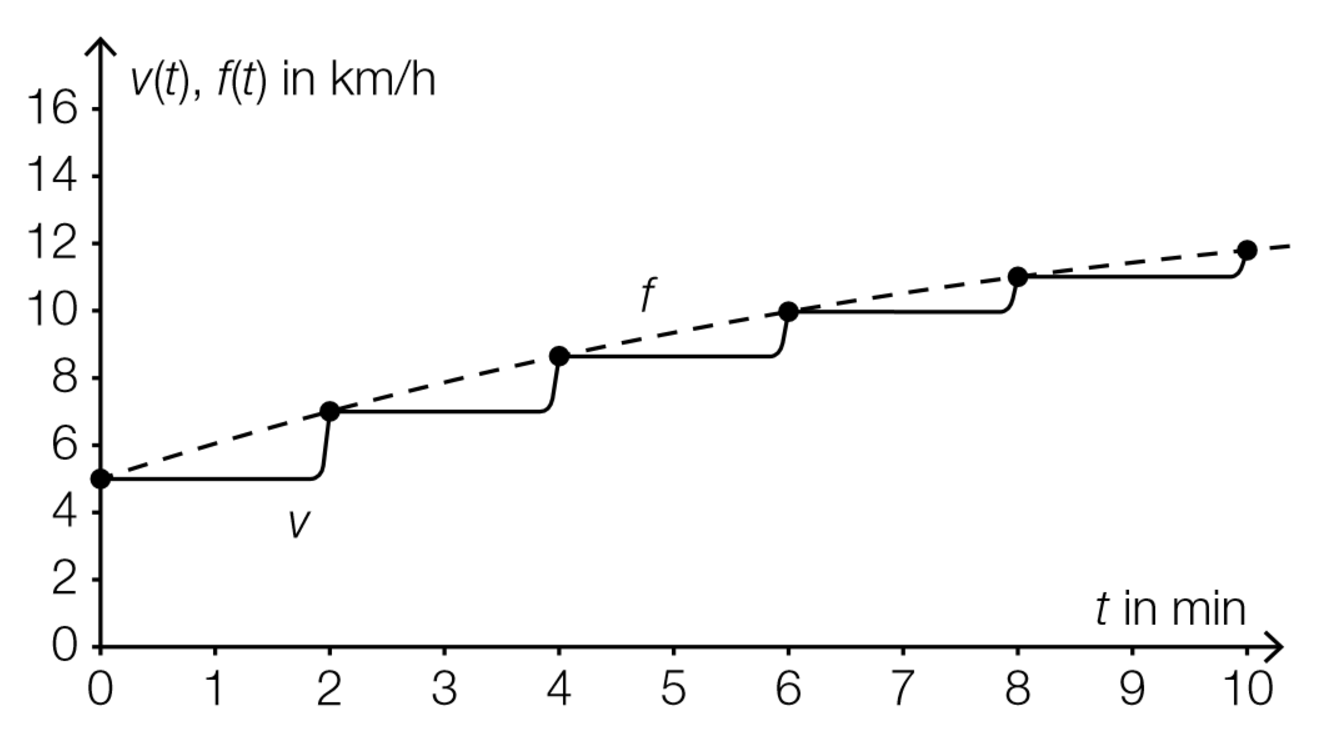
\includegraphics{../Bilder/Bild76-1.eps}}
\end{center}

\subsection{Aufgabenstellung:}
\begin{enumerate}
	\item Gib einen Ausdruck an, mit dem das arithmetische Mittel der Laufbandgeschwindigkeiten während des 30-minütigen Trainingsprogramms berechnet werden kann, und ermittle diesen Wert!\leer
	
	Begründe, warum das arithmetische Mittel der Laufbandgeschwindigkeiten der mittleren Geschwindigkeit $\bar{v}$ während des 30-minütigen Trainingsprogramms entspricht!
	
	Berechne unter Verwendung der mittleren Geschwindigkeit $\bar{v}$ die während des 30-minütigen Trainingsprogramms bewältigte Strecke!
	
	\item Gib die minimale und die maximale Geschwindigkeit des Laufbands während des 30-minütigen Trainingsprogramms an!\leer
	
	$v_\text{min}=$ \rule{5cm}{0.3pt}\,km/h\leer
	
	$v_\text{max}=$ \rule{5cm}{0.3pt}\,km/h\leer
	
	Begründe, warum zu den Zeitpunkten $t_{\text{min}}$ und $t_{\text{max}}$, zu denen die minimale bzw. die maximale Geschwindigkeit des Laufbands in dem 30-minptigen Trainingsprogramm erreicht wird, $f'(t_{\text{min}})\neq 0$ und $f'(t_\text{max})\neq 0$ gilt!\leer
	
	\item Gib den Wert von $v'(1)$ an und interpretiere diesen Wert (mit Angabe der Einheit) im gegebenen Kontext!\leer
	
	$v'(1)=$ \rule{5cm}{0.3pt}\leer
	
	Beschreibe anhand des Graphen in der Einleitung, wie der Graph der Ableitungsfunktion $v'$ im Intervall $[0;30]$ verlaufen müsste!\leer
	
	\item Die in den ersten zehn Trainingsminuten zurückgelegte Weglänge kann näherungsweise mit dem Integral $\frac{1}{60}\cdot\int^{10}_0{f(t)}$d$t$ berechnet werden.
	
	Berechne diesen Näherungswert und erläuter die Bedeutung des Faktors $\frac{1}{60}$!\leer
	
	Gib die absolute Abweichung des berechneten Näherungswertes von der tatsächlich zurückgelegten Weglänge während der ersten zehn Minuten in Metern an!	\leer
	
	\item Unter bestimmten Voraussetzungen ist der Energiebedarf einer Person bei einem Lauftraining direkt proportional zur Masse der Person (in kg) und zur zurückgelegten Weglänge (in km).

Die nachstehende Tabelle zeigt den Energiebedarf (in kcal) einer 80\,kg schweren Person bei einem Lauftraining in Abhängigkeit von der Dauer $t$ des Trainings. Die Person läuft mit einer konstanten Geschwindigkeit von 10\,km/h.

\begin{center}
	\begin{tabular}{|l|l|l|l|l|}\cline{2-5}
	\multicolumn{1}{c|}{}&$t=15$\,min&$t=30$\,min&$t=45$\,min&$t=60$\,min\\ \hline
	Energiebedarf in kcal&194&388&582&776\\ \hline	
	\end{tabular}
\end{center}

Zeige anhand der Tabellenwerte die direkte Proportionalität des Energiebedarfs zur zurückgelegten Wegstrecke und berechne den Proportionalitätsfaktor $k$!

Beim Lauftraining wird die Geschwindigkeit häufig als "`Tempo"' in min/km umschrieben. Berechne für die unten angeführten Geschwindigkeiten unter Verwendung des Proportionalitätsfaktors $k$ für eine 90\,kg schwere Person jeweils das Tempo und den Energiebedarf (in kcal) für die angegebene Zeitdauer!

\begin{center}
	\begin{tabular}{|p{3cm}|p{3cm}|p{3cm}|p{3cm}|}\hline
	\multirow{2}{2cm}{Geschwindigkeit in km/h}&\multirow{2}{2cm}{Tempo in min/km}&\multirow{2}{2cm}{Energiebedarf in 15\,min}&\multirow{2}{2cm}{Energiebedarf in 30\,min}\\
	&&&\\ \hline \hline
	\multicolumn{1}{|c|}{7,5}&\multicolumn{1}{c|}{8}&&\\ \hline
	\multicolumn{1}{|c|}{10}&&&\\ \hline
	\multicolumn{1}{|c|}{12}&&&\\ \hline	
	\end{tabular}
\end{center}
\end{enumerate}

\antwort{
\begin{enumerate}
	\item \subsection{Lösungserwartung:} 

$\bar{v}=\frac{1}{15}\cdot(f(0)+f(2)+f(4)+...+f(28)\approx 11,57$

Das arithmetische Mittel der Laufbahngeschwindigkeiten beträgt 11,57\,km/h\leer

Das Arithmetische Mittel entspricht der mittleren Geschwindigkeit während des 30-minütigen Trainingsprogramms, weil die Geschwindigkeiten $v(0),...,v(28)$ in gleich langen Zeitintervallen (2\,min) jeweils konstant sind.\leer

zurückgelegte Weglänge: $0,5\,\text{h}\cdot 11,57\,\text{km/h}=5,785$\,km

	\item \subsection{Lösungserwartung:}
	
	$v_\text{min}=5$\,km/h
	
	$v_\text{max}=14,16$\,km/h\leer
	
	$t_\text{min}$ und $t_\text{max}$ sind keine lokalen Extremstellen der Funktion $f$, weshalb die 1. Ableitung von $f$ an diesen Stellen nicht null ist.

\item \subsection{Lösungserwartung:}
	
$v'(1)=0$

Mögliche Interpretationen:

Die Beschleunigung (momentane Geschwindigkeitsänderung) des Laufbands nach 1 Minute beträgt 0\,m/s$²$.

oder:

Das Laufband (die Läuferin/der Läufer) bewegt sich während der ersten 2 Minuten mit konstanter Geschwindigkeit, d.h., seine Beschleunigung ist zum Zeitpunkt $t=1$\,min gleich null.\leer

Der Graph von $v'$ würde auf der 1. Achse verlaufen und nur zu den Zeitpunkten der Geschwindigkeitsänderungen $(t=2, t=4, t=6,...)$ sehr hohe Werte annehmen.

\item \subsection{Lösungserwartung:}
	
$\frac{1}{60}\cdot\int^{10}_0{f(t)}$d$t\approx 1,506$

zurückgelegte Weglänge: ca. 1,51\,km\leer

Mögliche Begründungen:

Der Faktor $\frac{1}{60}$ ist erforderlich, um die Geschwindigkeiten von km/h in km/min umzurechnen, da die Zeiten (Intervallgrenzen) in Minuten gegeben sind (1\,h=60\,min).

oder:

Der Faktor $\frac{1}{60}$ ist erforderlich, um die pro Stunde zurückgelegten Wegstrecken auf die pro Minute zurückgelegten Wegstrecken umzurechnen.\leer

Für die tatsächlich zurückgelegte Weglänge gilt:

$\frac{2}{60}\cdot(f(0)+f(2)+f(4)+f(6)+f(8))\approx 1,388$\,km

$\Rightarrow$ Der Näherungswert für die Weglänge weicht um ca. 118\,m vom exakten Wert ab.

\item \subsection{Lösungserwartung:}
	
$194=k\cdot 80\cdot 2,5$

$k=0,97$\leer

Bei der doppelten/dreifachen/vierfachen Laufzeit wird die doppelte/dreifache/vierfache Strecke zurückgelegt und auch der Energiebedarf ist doppelt/dreimal/viermal so groß.

\begin{center}
	\begin{tabular}{|p{3cm}|p{3cm}|p{3cm}|p{3cm}|}\hline
	\multirow{2}{2cm}{Geschwindigkeit in km/h}&\multirow{2}{2cm}{Tempo in min/km}&\multirow{2}{2cm}{Energiebedarf in 15\,min}&\multirow{2}{2cm}{Energiebedarf in 30\,min}\\
	&&&\\ \hline \hline
	\multicolumn{1}{|c|}{7,5}&\multicolumn{1}{c|}{8}&\cellcolor[gray]{0.7}163,7&\cellcolor[gray]{0.7}327,4\\ \hline
	\multicolumn{1}{|c|}{10}&\cellcolor[gray]{0.7}6&\cellcolor[gray]{0.7}218,25&\cellcolor[gray]{0.7}436,5\\ \hline
	\multicolumn{1}{|c|}{12}&\cellcolor[gray]{0.7}5&\cellcolor[gray]{0.7}261,9&\cellcolor[gray]{0.7}523,8\\ \hline	
	\end{tabular}
\end{center}

\end{enumerate}}
		\end{langesbeispiel}%
\hrule  \leer

\section{78 - MAT - AG 2.4, AN 4.2, AN 4.3, FA 1.4, FA 1.7, FA 3.2, FA 4.1, FA 5.6, WS 1.1, WS 1.2 - Einkommensverteilung - BIFIE Aufgabensammlung}

\begin{langesbeispiel} \item[0] %PUNKTE DES BEISPIELS
	
Der Statistiker Max Lorenz beschrieb bereits im Jahr 1905 statistische Verteilungen mithilfe der nach ihm benannten Lorenz-Kurve. Eine Lorenz-Kurve $f$ kann z.B. zur Beschreibung er Einkommensverteilung in einem Staat herangezogen werden. Je ausgepr�gter ihr "`Bauch"' ist, desto gr��er ist der Einkommensunterschied zwischen niedrigem und hohem Einkommen.

Die Lorenz-Kurve der Einkommensverteilung eines Staates, in dem alle Personen bis auf eine Person nichts verdienen und diese eine Person alles bekommt, wird in der nachstehenden Grafik durch die punktrierten Linien (Katheten eines rechtwinkeligen Dreiecks) dargestellt. Das andere Extrem ist ein Staat, in dem alle Personen gleich viel verdienen. In diesem Fall die die Lorenz-Kurve zu einer Geraden $h$, welche durch die strichlierte Linie dargestellt ist. Zwischen den beiden Extremen verl�uft die Lorenz-Kurve $f$ eines Staates.\leer

Jeder Punkt $P=(x|f(x))$ auf der Kurve $f$ steht f�r folgende Aussage: Die einkommensschw�chsten $x$\,\% aller Haushalte beziehen $f(x)$\,\% des Gesamteinkommens."'

\begin{center}
	\resizebox{0.7\linewidth}{!}{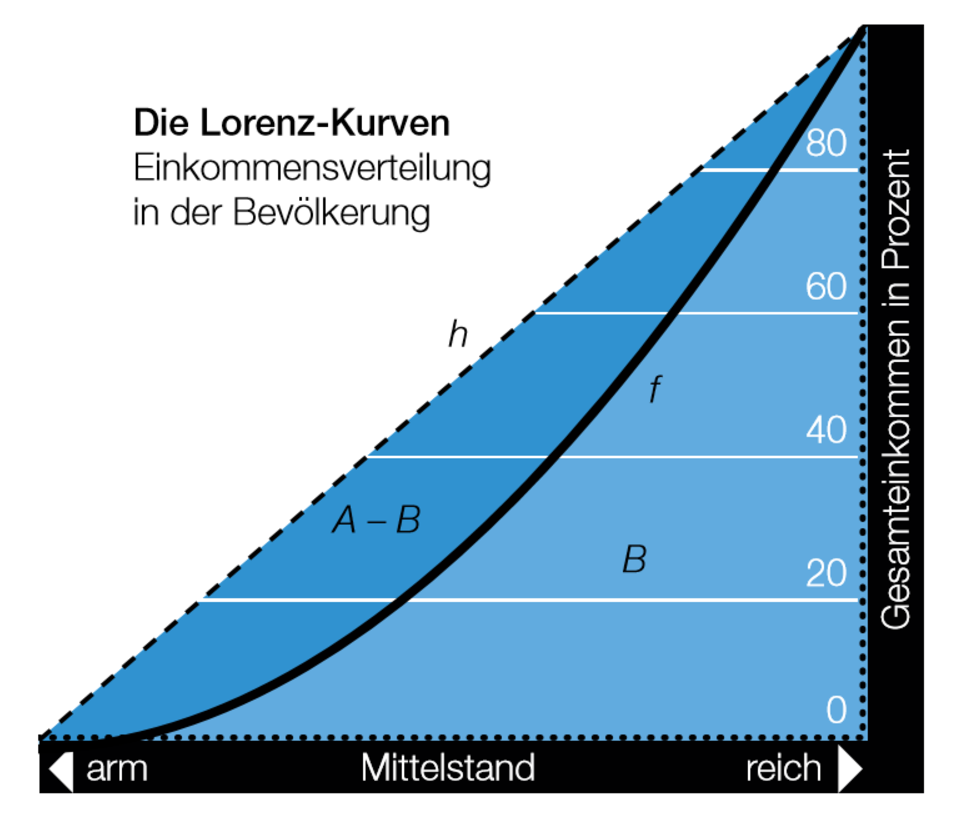
\includegraphics{../Bilder/Bild78-1.eps}}
\end{center}

Der Fl�cheninhalt des rechtwinkligen Dreiecks wird mit $A$ bezeichnet. Der Graph der Lorenz-Kurve $f$ schlie�t mit den beiden Katheten des rechtwinkeligen Dreiecks eine Fl�che mit Inhalt $B$ ein. Setzt man den Inhalt der Fl�che zwischen der Lorenz-Kurve $f$ und der Geraden $h$ mit der Dreiecksfl�che $A$ in Bezug, erh�lt man den Gini-Ungleichheitskoeffizienten $GUK=\frac{A-B}{A}$, eine Zahl zwischen null und ein. Je kleiner der GUK ist, desto gleichm��iger ist das Gesamteinkommen auf die Bev�lkerung verteilt.\leer

In der nachstehenden Grafik ist die Einkommensverteilung in �sterreich in Prozent der gesamten Bruttobez�ge im jahr 2006 dargestellt. Daraus ist z.B. abzulesen, dass jene 20\,\% der Bev�lkerung mit den niedrigsten Bruttoeinkommen nur 2,2\,\% des Gesamtbruttoeinkommens erhalten haben.

\begin{center}
	\resizebox{0.8\linewidth}{!}{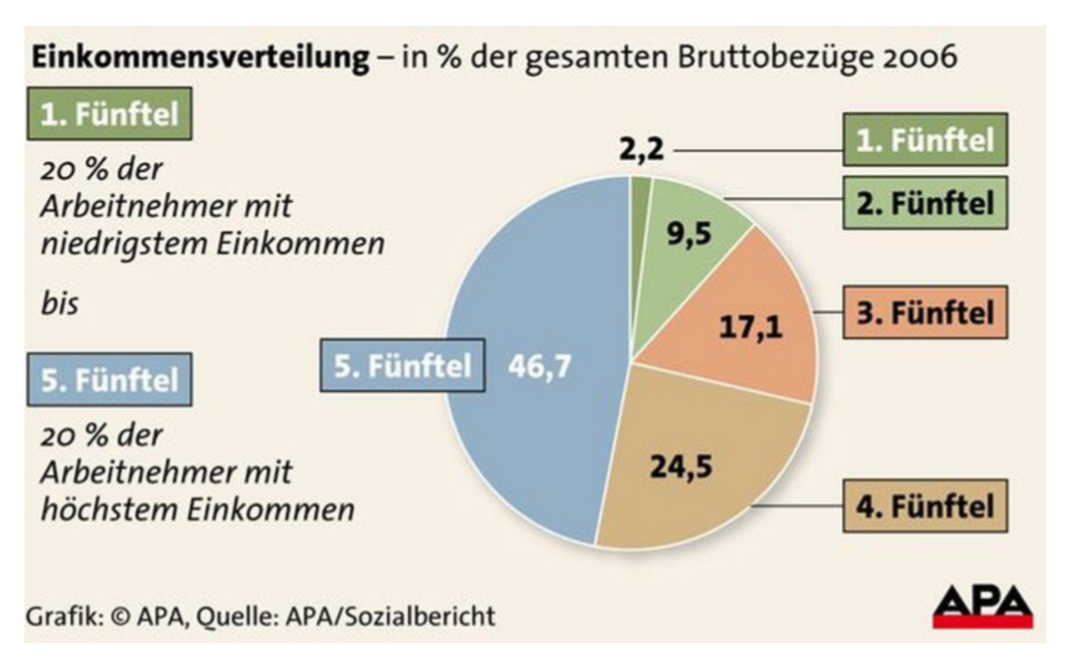
\includegraphics{../Bilder/Bild78-2.eps}}
\end{center}

\begin{scriptsize}\begin{singlespace}Quelle: http://diepresse.com/home/wirtschaft/economist/446997/Sozialbericht\_Einkommen-in-Oesterreich-ungleicher-verteilt [04.05.2017].\end{singlespace}\end{scriptsize}

\subsection{Aufgabenstellung:}
\begin{enumerate}
	\item Zeichne die Lorenzkurve f�r die Einkommensverteilung der Bruttobez�ge in �sterreich im Jahr 2006 in den nachstehenden Grafik als Streckenzug ein!
	
	\begin{center}
		\resizebox{0.8\linewidth}{!}{\psset{xunit=8.0cm,yunit=8.0cm,algebraic=true,dimen=middle,dotstyle=o,dotsize=4pt 0,linewidth=0.8pt,arrowsize=3pt 2,arrowinset=0.25}
\begin{pspicture*}(-0.08726875556452825,-0.12333898008375876)(1.1526748130814817,1.0658128492748549)
\multips(0,0)(0,0.1){12}{\psline[linestyle=dashed,linecap=1,dash=1.5pt 1.5pt,linewidth=0.4pt,linecolor=lightgray]{c-c}(0,0)(1.1526748130814817,0)}
\multips(0,0)(0.2,0){7}{\psline[linestyle=dashed,linecap=1,dash=1.5pt 1.5pt,linewidth=0.4pt,linecolor=lightgray]{c-c}(0,0)(0,1.0658128492748549)}
\psaxes[labelFontSize=\scriptstyle,xAxis=true,yAxis=true,Dx=0.2,Dy=0.1,ticksize=-2pt 0,subticks=2]{->}(0,0)(0.,0.)(1.1526748130814817,1.0658128492748549)
\begin{scriptsize}
\rput[tl](0.023837298973644686,1.0368091461197668){Einkommensanteil (relativ)}
\rput[tl](0.5727012083922189,0.05068323884677006){Einkommensgruppe (Anteil relativ)}
\psline[linewidth=1.2pt,linestyle=dashed,dash=1pt 1pt](0.,0.)(1.,1.)
\rput[tl](0.5660348451199285,0.6275346682646341){h}
\psline[linewidth=1.2pt]{->}(0.7,-0.09)(0.89,-0.09)
\psline[linewidth=1.2pt]{->}(0.49,-0.09)(0.3,-0.09)
\rput[tl](0.49937121239702476,-0.07983342535112656){Mittelstand}
\rput[tl](0.92,-0.075){reich}
\rput[tl](0.2,-0.07983342535112656){arm}
\end{scriptsize}
\end{pspicture*}}
	\end{center}
	
	Berechne mithilfe des eingezeichneten Streckenzuges den GUK f�r die Bruttobez�ge in �sterreich f�r das Jahr 2006!\leer
	
	\item Die Verteilung der Bruttoeinkommen in �sterreich im Jahr 2006 soll durch eine Polynomfunktion $p$ so modelliert werden, dass alle Daten, die aus dem Kreisdiagramm aus der Einleitung abgelesen werden k�nnen mit Funktionswerten dieser Polynomfunktion �bereinstimmen.\leer
	
	Begr�nde, welchen Grad die Polynomfunktion $p$ bei konkreter Berechnung (maximal) hat!\leer
	
	Begr�nde, warum eine Exponentialfunktion $e$ mit $e(x)=a\cdot b^x (a,b\in\mathbb{R}^+$ nicht f�r die Modellierung einer Lorenz-Kurve geeignet ist!\leer
	
	\item Um politische Ma�nahmen absch�tzen zu k�nnen, werden verschiedene Szenarien entworfen. So soll beispielsweise f�r die Bruttoeinkommen langfristig eine Lorenz-Kurve angestrebt werden, die durch die Funktion $g$ mit der Funktionsgleichung $g(x)=0,245\cdot x�+0,6\cdot x�+0,155\cdot x$ beschrieben werden kann.\leer
	
	Gib eine Gleichung an, mit der der GUK f�r die angestrebte Einkommensverteilung berechnet werden kann, und ermittle diesen GUK!\leer
	
	Gib mithilfe konkreter Zahlenwerte an, wie sich in diesem Fall die Einkommensverteilung der "`20\,\% der Arbeitnehmer/innen mit den niedrigsten Bruttoeinkommen"' und die Einkommensverteilung der "`20\,\% der Arbeitnehmer/innen mit den h�chsten Bruttoeinkommen"' im Vergleich zu den Bruttobez�gen im Jahr 2006 in �sterreich �ndern w�rde!\leer
	
	\item F�r das Jahr 2007 kann die Einkommensverteilung f�r �sterreich mit einem GUK von $0,26$ beschrieben werden.
	
	\begin{scriptsize}\begin{singlespace}Datenquelle: https://de.wikipedia.org/wiki/Liste\_der\_L\%C3\%A4nder\_nach\_Einkommensverteilung [04.05.2017]. \end{singlespace}\end{scriptsize}\leer
	
	Angenommen, die Lorenz-Kurve f�r die Einkommenverteilung kann f�r ein bestimmtes Land, das eine ausgeglichenere Einkommensverteilung als �sterreich aufweisen soll, durch eine Potenzfunktion $h$ mit $h(x)=a\cdot x^z+b$ mit $a,b,z\in\mathbb{R}$ beschrieben werden.\leer
	
	Gib an, welche Werte die Parameter $a$ und $b$ haben m�ssen, und begr�nde deine Wahl!\leer
	
	Gib eine Ungleichung an, die f�r das Jahr 2007 einen Zusammenhang zwischen dem GUK von �sterreich und dem GUK von demjenigen Land, das eine ausgeglichenere Einkommensverteilung als �sterreich aufweisen soll, beschreibt! Ermittle f�r diesen Fall einen m�glichen Wert f�r den Exponenten $z$ mit $z>1$!
	
\end{enumerate}

\antwort{
\begin{enumerate}
	\item \subsection{L�sungserwartung:} 

\begin{center}
		\resizebox{0.8\linewidth}{!}{\psset{xunit=8.0cm,yunit=8.0cm,algebraic=true,dimen=middle,dotstyle=o,dotsize=4pt 0,linewidth=0.8pt,arrowsize=3pt 2,arrowinset=0.25}
\begin{pspicture*}(-0.08726875556452825,-0.12333898008375876)(1.1526748130814817,1.0658128492748549)
\multips(0,0)(0,0.1){12}{\psline[linestyle=dashed,linecap=1,dash=1.5pt 1.5pt,linewidth=0.4pt,linecolor=lightgray]{c-c}(0,0)(1.1526748130814817,0)}
\multips(0,0)(0.2,0){7}{\psline[linestyle=dashed,linecap=1,dash=1.5pt 1.5pt,linewidth=0.4pt,linecolor=lightgray]{c-c}(0,0)(0,1.0658128492748549)}
\psaxes[labelFontSize=\scriptstyle,xAxis=true,yAxis=true,Dx=0.2,Dy=0.1,ticksize=-2pt 0,subticks=2]{->}(0,0)(0.,0.)(1.1526748130814817,1.0658128492748549)
\begin{scriptsize}
\rput[tl](0.023837298973644686,1.0368091461197668){Einkommensanteil (relativ)}
\rput[tl](0.5727012083922189,0.05068323884677006){Einkommensgruppe (Anteil relativ)}
\psline[linewidth=1.2pt,linestyle=dashed,dash=1pt 1pt](0.,0.)(1.,1.)
\rput[tl](0.5660348451199285,0.6275346682646341){h}
\psline[linewidth=1.2pt]{->}(0.7,-0.09)(0.89,-0.09)
\psline[linewidth=1.2pt]{->}(0.49,-0.09)(0.3,-0.09)
\rput[tl](0.49937121239702476,-0.07983342535112656){Mittelstand}
\rput[tl](0.92,-0.075){reich}
\rput[tl](0.2,-0.07983342535112656){arm}
\psline[linewidth=1.2pt](0.,0.)(0.2,0.022)
\psline[linewidth=1.2pt](0.2,0.022)(0.4,0.117)
\psline[linewidth=1.2pt](0.4,0.117)(0.6,0.288)
\psline[linewidth=1.2pt](0.6,0.288)(0.8,0.533)
\psline[linewidth=1.2pt](0.8,0.533)(1.,1.)
\rput[tl](0.5060375756693152,0.18764517041246404){f}
\end{scriptsize}
\end{pspicture*}}
	\end{center}
	
	Der Inhalt der Fl�che zwischen dem Polygonzug $f$ und der Strecke $h$ betr�gt 0,208 Fl�cheneinheiten (die Ermittlung des Fl�cheninhalts zwischen der waagrechten Achse und dem Streckenzug kann z.B. aus zwei Dreiecksfl�chen und drei Trapezfl�chen erfolgen).\leer
	
	$\Rightarrow GUK=\frac{0,208}{0,5}=0,416$

	\item \subsection{L�sungserwartung:}
	
	Aus den Daten des Kreisdiagramms ergeben sich (f�r die Argumente $x=0, x=0,2, x=0,4, x=0,6, x=0,8, x=1$) sechs Funktionswerte von $p$ und somit sechs "`Bedingungen"' f�r die Koeffizienten der Funktionsgleichung. Eine Polynomfunktion f�nften Grades hat sechs Koeffizienten und ist daher geeignet.
	
	\textit{(Anmerkung: Bei "`besonderer"' Lage der Punkte kann auch ein Grad kleiner als f�nf ausreichend sein.}\leer
	
	Jede Lorenz-Kurve verl�uft durch den Punkt $(0|0)$. Da eine Exponentialfunktion $e$ mit $e(x)=a\cdot b^x$ $(a,b\in\mathbb{R}^+)$ nicht durch den Koordinatenursprung verl�uft, ist sie nicht f�r die Modellierung geeignet.

\item \subsection{L�sungserwartung:}
	
$GUK=\dfrac{0,5-\int^1_0{(0,245x�+0,6x�+0,155x)dx}}{0,5}=0,3225$\leer

$g(0,2)\approx 0,057$

$g(0,8)\approx 0,633$\leer

Der Einkommensanteil der "`20\,\% mit den niedrigsten Bruttoeinkommen"' w�rde (um ca. 3,5 Prozentpunkte) von 2,2\,\% auf ca. 5,7\,\% steigen.\leer

Der Einkommensanteil der "`20\,\% mit den h�chsten Bruttoeinkommen"' w�rde (um ca. 10 Prozentpunkte) von 46,7\,\% auf 36,7\,\% sinken.
\item \subsection{L�sungserwartung:}
	
$b=0$, da der Graph durch den Punkt $(0|0)$ verlaufen muss

$a=1$, da der Graph durch den Punkt $(1|1)$ verlaufen muss

$$\frac{0,5-\int^1_0{x^z}dx}{0,5}<0,26$$

$z\in\left(1;\frac{63}{37}\right)$

\end{enumerate}}
		\end{langesbeispiel}%
\hrule  \leer

\section{83 - MAT - WS 4.1, AN 1.2, AN 1.3, WS 1.3, WS 1.2 - Wachstumskurve von Kindern - Matura NT 1 16/17}

\begin{langesbeispiel} \item[6] %PUNKTE DES BEISPIELS

Um die Entwicklung der K�rperh�he und der Masse eines Kinder kontrollieren zu k�nnen, sind im Mutter-Kind-Pass die Perzentielenkurven f�r K�rperh�hen (Gr��e) und Masse angegeben (K�rperh�he in cm, Masse in kg). Perzentile teilen die K�rperh�hen und Massen der Kinder in Prozent-Bereiche auf. Liegt ein Wert auf dem 10. Wachstumsperzentil, so sind 10\,\% der Kinder des ausgew�hlten Alters kleiner oder gleich dem angegebenen Wert und 90\,\% gr��er oder gleich dem angegebenen Wert.

Es ist �blich, alle Werte zwischen dem 3. und dem 97. Perzentil als "`normal"' zu bezeichnen. Das folgende Diagramm zeigt die Wachstums- und K�rpermassekurven f�r Buben im Alter von 0 bis 18 Jahren:

\begin{center}
\resizebox{0.8\linewidth}{!}{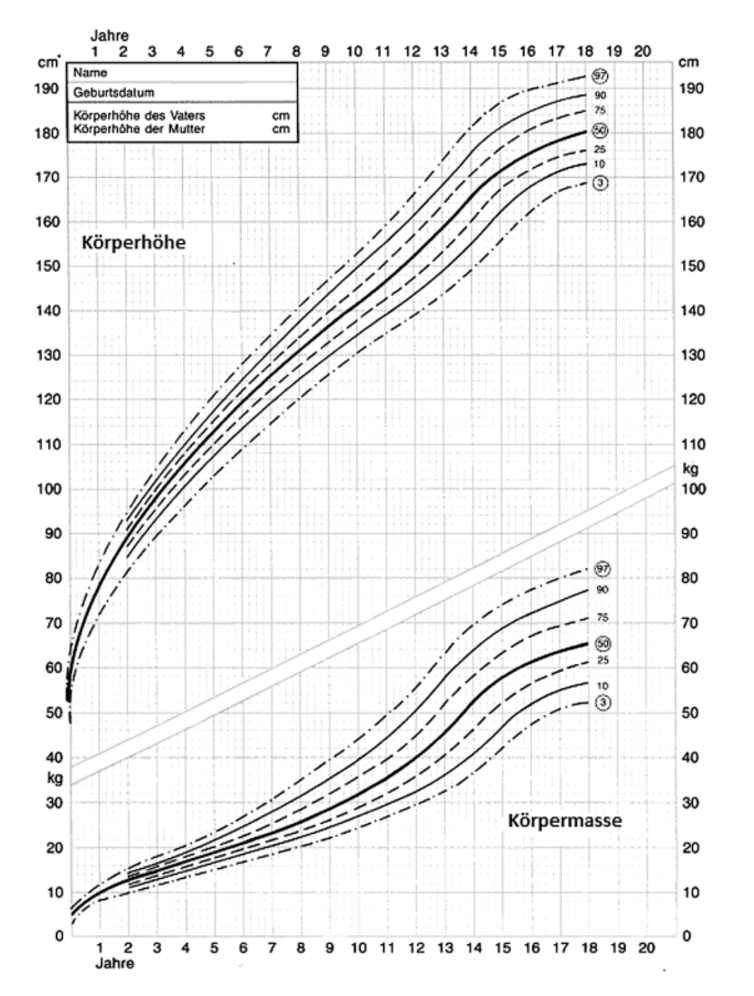
\includegraphics{../Bilder/Bild83-1.eps}}
\end{center}

\subsection{Aufgabenstellung:}
\begin{enumerate}
	\item Ein Schularzt untersucht eine zuf�llige Stichprobe von 8-j�hrigen Buben aus seinem Schulbezirk und erhebt unter anderem deren K�rpermassen (in kg). Anhand der Ergebnisse dieser Messung erstellt er f�r den Anteil der 8-j�hrigen Buben aus einem Schulbezirk, deren K�rpermasse im "`Normalbereich"' $[20\,\text{kg};35\,\text{kg}]$ liegt, das symmetrische Konfidenzintervall $[0,8535;0,9465]$ mit dem Konfidenzniveau $\gamma=0,95$.\leer
	
	Gib den Unterschied des der Berechnung zugrundeliegenden Stichprobenanteils zum Anteil der 8-j�hrigen Buben mit einer K�rpermasse im "`Normalbereich"' laut Diagramm in Prozentpunkten an!\leer
	
	Berechne die Anzahl der bei dieser Stichprobe gemessenen 8-j�hrigen Buben!\leer
	
	\item Angenommen, f�r ein bestimmtes Kind sind die K�rperh�hen $g(1),g(2),g(3),...$ zum ersten, zweiten, dritten usw. Geburtstag bekannt.
	
	Gib verbal oder als Formel an, wie sich die durchschnittliche Wachstumsgeschwindigkeit dieses Kindes in dem dreij�hrigen Zeitraum zwischen dem 6. und dem 9. Geburtstag bestimmen l�sst.\leer
	
	Betrache das Gr��enwachstum auf dem 50. Perzentil nach dem 8. Lebenjahr. Gib das ungef�hre Alter von Buben an, bei dem deren momentane Wachstumsgeschwindigkeit am gr��ten ist!\leer
	
	\item Gib an, welcher statistischen Kennzahl derjenige Wert entspricht, den man auf dem 50. Perzentil ablesen kann.\leer
	
	Erl�utere, welche Schwierigkeiten auftreten, wenn man aus dem angegebenen Diagramm ein Kastenschaubild (Boxplot) zur Darstellung der K�rperh�hen von 8-j�hrigen Buben erstellen m�chte!
	
	\end{enumerate}

\antwort{
\begin{enumerate}
	\item \subsection{L�sungserwartung:} 

Stichprobenanteil: 0,9

Anteil laut Diagramm: 0,94

Unterschied: 4 Prozentpunkte\leer

M�gliche Berechnung:

$0,9465=0,9+1,96\cdot\sqrt{\dfrac{0,9\cdot (1-0,9)}{n}}\Rightarrow\approx 160$ Buben
\subsection{L�sungsschl�ssel:}
\begin{itemize}
	\item Ein Punkt f�r die richtige L�sung.
	\item Ein Punkt f�r die richtige L�sung.
	
	Toleranzintervall: $[155\text{ Buben};165\text{ Buben}]$
	
	Die Aufgabe ist auch dann als richtig gel�st zu werten, wenn bei korrektem Ansatz das Ergebnis aufgrund eines Rechenfehlers nicht richtig ist.
\end{itemize}

	\item \subsection{L�sungserwartung:}

Die durchschnittliche Wachstumsgeschwindigkeit in diesem Zeitraum entspricht einem Drittel der Gr��enzunahme.

oder:

$\frac{g(9)-g(6)}{3}$\leer

Das ungef�hre Alter von Buben, bei dem deren momentane Wachstumsgeschwindigkeit am gr��ten ist, liegt bei ca. 13 Jahren.

\subsection{L�sungsschl�ssel:}
\begin{itemize}
	\item Ein Punkt f�r eine (sinngem��) korrekte Antwort bzw. eine richtige Formel. �quivalente Formeln sind als richtig zu werten.	
	\item Ein Punkt f�r die richtige L�sung, wobei die Einheit "`Jahre"' nicht angef�hrt sein muss.
	
	Toleranzintervall: $[12\text{ Jahre};14\text{ Jahre}]$
\end{itemize}

\item \subsection{L�sungserwartung:}

Die statistische Kennzahl, die demjenigen Wert entspricht, den man auf dem 50. Perzentil ablesen kann, ist der Median.

Die Schwierigkeiten bestehen darin, dass man zwar das 1. und das 3. Quartil sowie den Median, jedoch weder Minimum noch Maximum ablesen kann (und auch keine Informationen bez�glich Ausrei�ern hat).

\subsection{L�sungsschl�ssel:}
\begin{itemize}
	\item Ein Ausgleichspunkt f�r das Anf�hren der korrekten statistischen Kennzahl.
	\item Ein Punkt f�r eine (sinngem��) korrekte Erl�uterung.
\end{itemize}
\end{enumerate}}
		\end{langesbeispiel}%
\hrule  \leer

\section{86 - MAT - AG 2.1, FA 1.4, FA 2.2, FA 2.4, WS 1.1, WS 1.4 - Human Development Index - Matura 2016/17 2. NT}

\begin{langesbeispiel} \item[0] %PUNKTE DES BEISPIELS
Der Human Development Index ($HDI$) der Vereinten Nationen ist ein Wohlstandsindikator f�r L�nder, der eine Messung des Entwicklungsstandes des jeweiligen Landes erm�glichen sollte.
Der $HDI$ beinhaltet drei dimensionslose Gr��en (Lebenserwartungsindex ($LEI$), Bildungsindex ($BI$)
und Einkommensindex ($EI$)) und wird mit der Formel $HDI=\sqrt[3]{LEI \cdot BI \cdot EI}$ berechnet.

Dimensionslos bedeutet, dass diese Gr��en keine Einheiten haben.\leer

F�r die Berechnung des Indizes $LEI$ und $EI$ gilt seit 2010:

$LEI=\frac{LE-20}{85-20}$, wobei $LE$ die Lebenserwartung zum Zeitpunkt der Geburt in Jahren beschreibt

$EI=\frac{\ln(B)-\ln(100)}{\ln(75\,000)-\ln(100)}$, wobei $B$ das Bruttonationaleinkommen pro Kopf in US-Dollar (immer zu Jahresbeginn) beschreibt.\leer

Das Entwicklungsprogramm der Vereinten Nationen unterteilt die L�nder nach dem Wert des $HDI$ seit 2009 in vier Entwicklungskategorien:


\renewcommand{\arraystretch}{1.5}
\begin{center}
\begin{tabular}{c|c} \hline
\rowcolor{lightgray} Entwicklungskategorie eines Landes & Wert des $HDI$ \\ \hline
$E_1$ & $\leq 0,8$ \\ \hline
$E_2$ & $[0,7; 0,8)$ \\ \hline
$E_3$ & $[0,55; 0,7)$ \\ \hline
$E_4$ & $< 0,55$ \\ \hline
\end{tabular}
\end{center}
\tiny Datenquelle: Deutsche Gesellschaft f�r die Vereinten
Nationen (Hrsg.): Bericht �ber die menschliche Entwicklung
2015. Arbeit und menschliche Entwicklung. Berlin:
Berliner Wissenschafts-Verlag 2015, S. 240 \normalsize


Der $HDI$ einer Region in einem bestimmten Jahr ergibt sich aus dem arithmetischen Mittel der $HDI$s der zu dieser Region z�hlenden L�nder. \leer

Die Entwicklung des $HDI$ verschiedener Regionen zwischen 1980 und 2011 ist nachstehend abgebildet.

\begin{center}
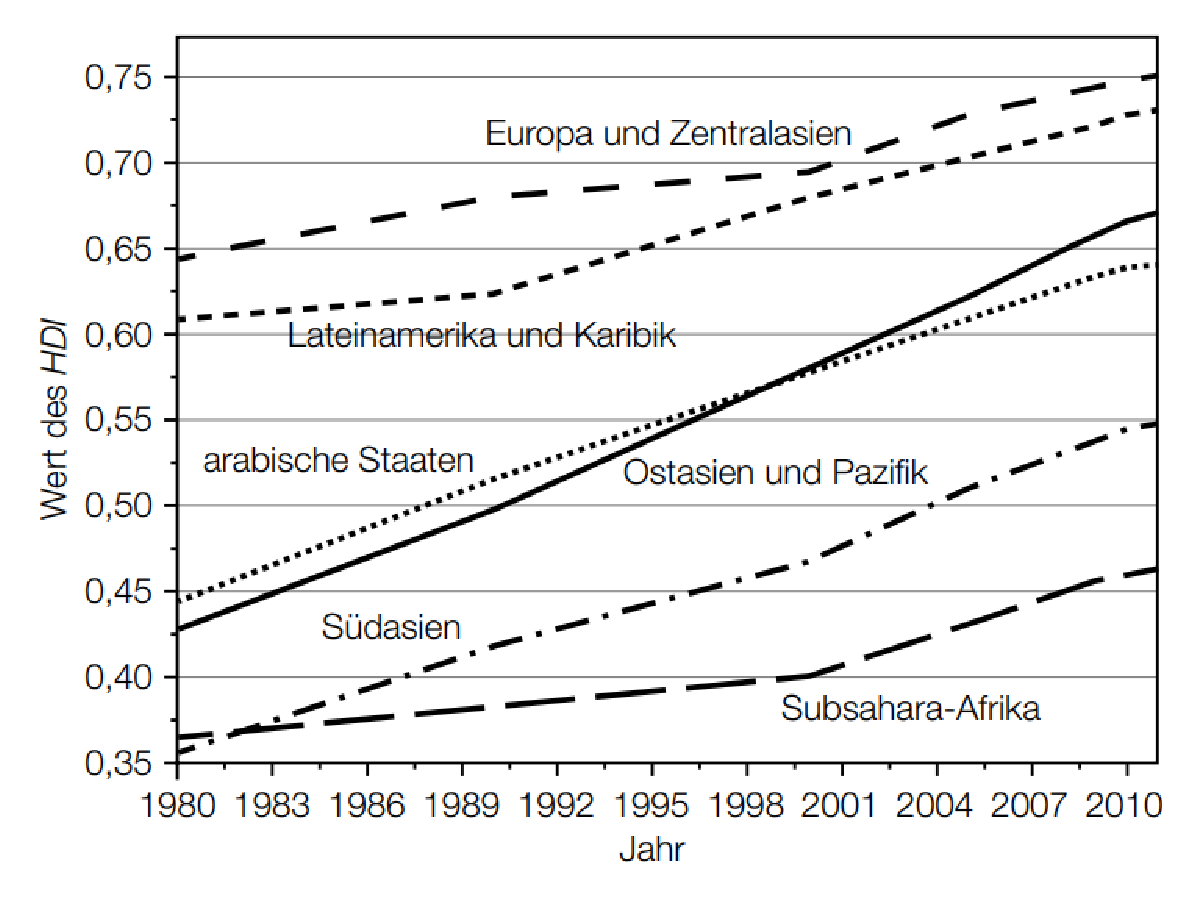
\includegraphics[width=0.7\textwidth]{../Bilder/Bild86-1.eps}
\end{center}
\begin{singlespace}
\tiny Datenquelle: https://de.wikipedia.org/wiki/
Index\_der\_menschlichen\_Entwicklung\#/
media/File:Human-Development-IndexTrends-2011.svg
[08.06.2017]. \normalsize
\end{singlespace}

\subsection{Aufgabenstellung:}

\begin{enumerate}
	\item F�r �sterreich wurde im Human Development Report f�r das Jahr 2013 die Lebenserwartung mit $LE = 81,1$ Jahren und der Bildungsindex mit $BI = 0,819$ angegeben. Die nachstehende Abbildung zeigt f�r die Jahre 2000 bis 2013 (jeweils zu Jahresbeginn) das Bruttonationaleinkommen �sterreichs pro Kopf in US-Dollar.
	
\begin{center}
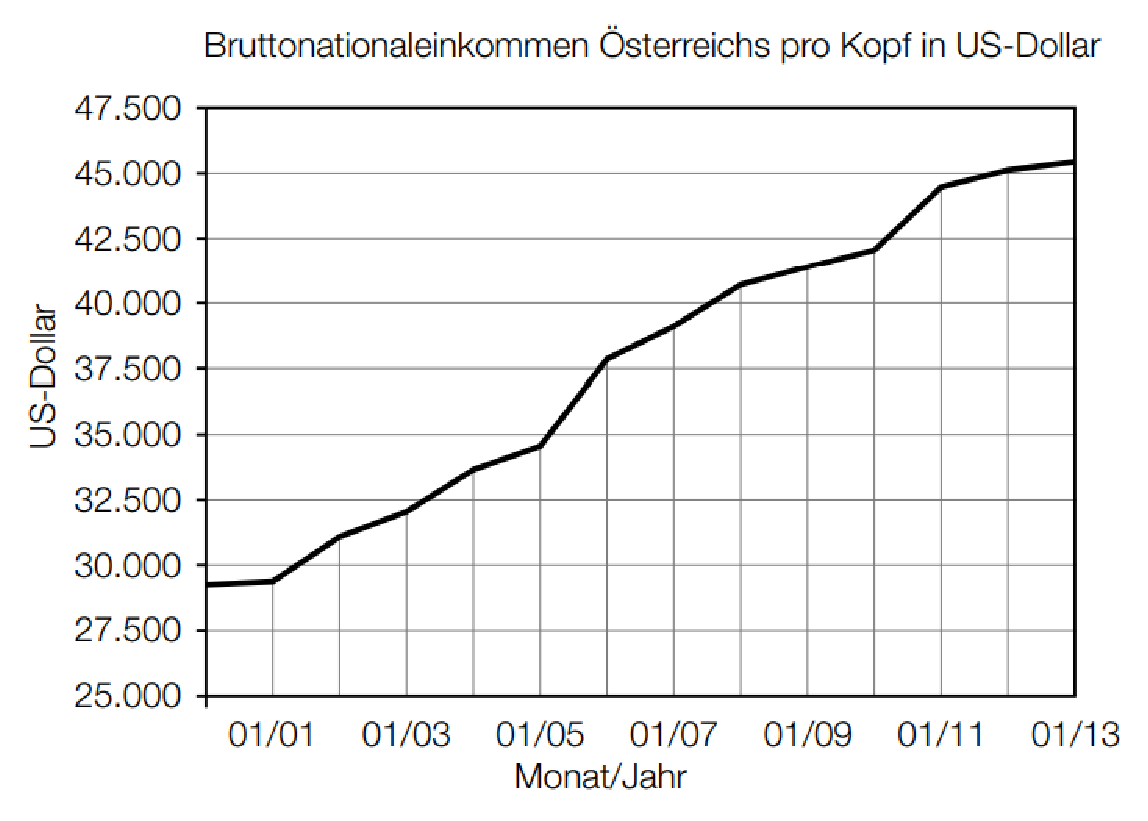
\includegraphics[width=0.6\textwidth]{../Bilder/Bild86-2.eps}
\end{center}	
\tiny Datenquelle: http://www.factfish.com/de/statistik/bruttonationaleinkommen [08.06.2017]. \normalsize

Ermittle f�r das Jahr 2013 den $HDI$ von �sterreich $(=HDI_{2013})$!\leer

Der $HDI$ von �sterreich f�r das Jahr 2013 $(HDI_{2013})$ war um ca. 2,5\,\% gr��er als der $HDI$ von �sterreich f�r das Jahr 2008 $(HDI_{2008})$. Gib eine Gleichung an, die diesen Zusammenhang beschreibt, und berechne den $HDI_{2008}$!

\item Die j�hrliche Entwicklung des $HDI$ der Region "`arabische Staaten"' kann im Zeitraum von 1980 bis 2010 n�herungsweise durch eine lineare Funktion $H$ mit der Gleichung $H(t) = k \cdot t + d$ mit $k, d \in \mathbb R$ und $t$ in Jahren beschrieben werden, wobei $H(0)$ dem Wert des Jahres 1980 entspricht.\leer

Bestimme die Werte der Parameter $k$ und $d$!\leer

Begr�nden Sie anhand der entsprechenden Abbildung, in welcher Region/in welchen Regionen die mittlere j�hrliche Zunahme des $HDI$ im Zeitraum von 1980 bis 2010 am ehesten jener der
Region "`arabische Staaten"' entsprach!

\item \fbox{A} Ermittle aus der entsprechenden Abbildung diejenige Jahreszahl, ab der die Region "`Lateinamerika und Karibik"' die Entwicklungskategorie $E_2$ aufweist!\leer

Gilt ab diesem Zeitpunkt sicher, dass ungef�hr die H�lfte der zu dieser Region z�hlenden L�nder
eine Entwicklungskategorie $E_2$ aufweist? Begr�nde deine Antwort!	
\end{enumerate}

\antwort{
\begin{enumerate}
	\item \subsubsection{L�sungserwartung:}

$LEI=\dfrac{81,1-20}{85-20}=0,94$

$EI\approx \dfrac{\ln(45\,400)-\ln(100)}{\ln(75\,000)-\ln(100)}\approx 0,924$

$HDI_{2013}=\sqrt[3]{0,94\cdot 0,819 \cdot 0,924} \approx 0,893$

$HDI_{2013}=HDI_{2008}\cdot 1,025$

$HDI_{2008}\approx 0,871$

\subsubsection{L�sungsschl�ssel}

- Ein Punkt f�r die richtige L�sung.
Toleranzintervall: $[0,88; 0,91]$
Die Aufgabe ist auch dann als richtig gel�st zu werten, wenn bei korrektem Ansatz das Ergebnis
aufgrund eines Rechenfehlers nicht richtig ist.
- Ein Punkt f�r eine korrekte Gleichung und die richtige L�sung. �quivalente Gleichungen sind
als richtig zu werten.
Toleranzintervall: $[0,85; 0,89]$

\item \subsubsection{L�sungserwartung:}

$k=\dfrac{0,64-0,44}{30}=0,006\dot{6}$

$d=0,44$

In der Region "`S�dasien"' entsprach die mittlere j�hrliche Zunahme des HDI im Zeitraum 1980 bis 2010 am ehesten jener der Region "`arabische Staaten"'.

M�gliche Begr�ndung:\\
Die Sekanten durch die Punkte $(1980|0,44)$ und $(2010|0,64)$ sowie $(1980|0,36)$ und $(2010|0,54)$ verlaufen ann�hernd parallel zueinander. 

\subsubsection{L�sungsschl�ssel:}

- Ein Punkt f�r die Angabe der beiden korrekten Werte.
Toleranzintervall f�r $k$: $[0,005; 0,01]$
Toleranzintervall f�r $d$: $[0,43; 0,45]$
- Ein Punkt f�r die Angabe der Region "`S�dasien"' und f�r eine (sinngem��) korrekte Begr�ndung.

\item \subsubsection{L�sungserwartung:}

Ab dem Jahr 2004 weist die Region "`Lateinamerika und Karibik"' die Entwicklungskategorie $E_2$
auf.\leer

Nein, es gilt nicht als sicher, dass ab diesem Zeitpunkt ungef�hr die H�lfte der zu dieser Region
z�hlenden L�nder die Entwicklungskategorie $E_2$ aufweist.


M�gliche Begr�ndung:
Wenn eine sehr kleine Anzahl an L�ndern mit sehr hohen HDI-Werten einer gro�en Anzahl an
L�ndern mit niedrigen $HDI$-Werten $(< 0,7)$ gegen�bersteht, kann dennoch das arithmetische
Mittel der $HDI$s gr��er als $0,7$ sein, ohne dass ungef�hr die H�lfte der zu dieser Region z�hlenden
L�nder die Entwicklungskategorie $E_2$ aufweist.

\subsubsection{L�sungsschl�ssel:}

- Ein Ausgleichspunkt f�r die richtige L�sung.
Toleranzintervall: $[2003; 2005]$
- Ein Punkt f�r eine richtige Antwort und eine korrekte Begr�ndung. Andere korrekte Begr�ndungen
(z.B. anhand sinnvoller Zahlenbeispiele oder mit der Feststellung, dass das arithmetische
Mittel nicht notwendigerweise der Median sein muss) sind ebenfalls als richtig zu
werten.

\end{enumerate}
}

		
\end{langesbeispiel}%
\hrule  \leer

\section{87 - MAT - AN 3.2, AN 3.2, AN 4.3, AN 4.2, WS 3.2 - Dichtefunktion und Verteilungsfunktion - Matura 2016/17 2. NT}

\begin{langesbeispiel} \item[3] %PUNKTE DES BEISPIELS
						Es sei $X$ eine Zufallsvariable, für die sich die Wahrscheinlichkeit, dass $X$ in einem Intervall $I$ liegt, mithilfe einer sogenannten Dichtefunktion $f$ folgendermaßen ermitteln lässt:
						
						$P(a\leq X\leq b)=\displaystyle\int^b_a f(x)$d$x$ für alle $a,b\in I$ mit $a\leq b$
						
						In diesem Fall gilt für die Verteilungsfunktion $F:F(x)=P(X\leq x)$ für alle $x\in\mathbb{R}$, d.h. insbesondere $F(b)-F(a)=P(a\leq X\leq b)$ für $a,b\in I$ und $a\leq b$.
						
						Die nachstehende Grafik zeigt den Graphen einer Dichtefunktion $f$ mit $f(x)=k\cdot\sin(x)$ für $x\in[0;c]$, wobei $k\in\mathbb{R}, k>0$ und $f(c)=0$ gilt. Für $x\neq[0;c]$ gilt: $f(x)=0$.
						
						\begin{center}
							\resizebox{0.8\linewidth}{!}{\psset{xunit=4.0cm,yunit=4.0cm,algebraic=true,dimen=middle,dotstyle=o,dotsize=5pt 0,linewidth=1.6pt,arrowsize=3pt 2,arrowinset=0.25}
\begin{pspicture*}(-0.1490384615384615,-0.1384157660521301)(3.2980769230769234,1.2816274634456448)
\psaxes[labelFontSize=\scriptstyle,xAxis=true,yAxis=true,labels=y,Dx=0.2,Dy=1.,yticksize=-2pt 0,xticksize=0]{->}(0,0)(0.,0.)(3.2980769230769234,1.2816274634456448)[x,140] [f(x),-40]
\psplot[linewidth=2.pt,plotpoints=200]{0}{3.14}{0.5*SIN(x)}
\antwort{\psplot[linewidth=2.pt,plotpoints=200]{0}{3.14}{-1.0/2.0*COS(x)+0.5}}
\rput[tl](3.1153846153846154,-0.03075905912269592){c}
\rput[tl](2.331730769230769,0.5075244755244751){$f$}
\antwort{\rput[tl](2.394230769230769,1.0406815003178636){$F$}}
\end{pspicture*}}
						\end{center}

				\subsection{Aufgabenstellung:}
\begin{enumerate}
	\item Gib für die gegebenen Dichtefunktion $f$ den Funktionswert $F(0)$ der zugehörigen Verteilungsfunktion $F$ an und begründe, warum $F(c)=1$ ist!\leer
	
	$F(0)=$\,\antwort[\rule{3cm}{0.3pt}]{0}
	
	Skizziere in der oben stehenden Grafik den Graphen der zugehörigen Verteilungsfunktion $F$ und beschreibe das Krümmungsverhalten von $F$ im Intervall $[0;c]$!
	
	\item Gib an, durch welche Eigenschaft von $f$ der Wert des Parameters $k$ festgelegt ist, und berechne den Wert von $k$!
	
	Gib einen Term der zugehörigen Verteilungsfunktion $F$ im Intervall $[0;c]$ an!\leer
	
	$F(x)=$\,\antwort[\rule{3cm}{0.3pt}]{$-0,5\cdot\cos(x)+0,5$}
	
	\item Für ein Ereignis $E$ gilt: $P(E)=1-P(X\leq c-a)$ für ein beliebiges $a\in[0;c]$.
	
	\fbox{A} Beschreibe dieses Ereignis $E$ verbal!
	
	Stelle für $a\leq\frac{c}{2}$ die Wahrscheinlichkeit $P(a\leq X\leq c-a)$ in nachstehender Grafik als Fläche dar und begründe den Zusammenhang \\ \mbox{$P(a\leq X\leq c-a)=1-2\cdot P(X\leq a)$} anhand dieser Darstellung!
	
	\begin{center}
		\resizebox{0.8\linewidth}{!}{\psset{xunit=4.0cm,yunit=4.0cm,algebraic=true,dimen=middle,dotstyle=o,dotsize=5pt 0,linewidth=1.6pt,arrowsize=3pt 2,arrowinset=0.25}
\begin{pspicture*}(-0.1490384615384615,-0.1384157660521301)(3.2980769230769234,1.2816274634456448)
\psaxes[labelFontSize=\scriptstyle,xAxis=true,yAxis=true,labels=y,Dx=0.2,Dy=1.,yticksize=-2pt 0,xticksize=0]{->}(0,0)(0.,0.)(3.2980769230769234,1.2816274634456448)[x,140] [f(x),-40]
\psplot[linewidth=2.pt,plotpoints=200]{0}{3.14}{0.5*SIN(x)}
\rput[tl](3.1153846153846154,-0.0307){c}
\rput[tl](2.331730769230769,0.5075244755244751){$f$}
\antwort{\pscustom[linewidth=0.8pt,fillcolor=black,fillstyle=solid,opacity=0.1]{\psplot{1.0471975511965976}{2.0943951023931953}{0.5*SIN(x)}\lineto(2.0943951023931953,0)\lineto(1.0471975511965976,0)\closepath}
\rput[tl](1.0144230769230769,-0.0307){$a$}
\rput[tl](2.0,-0.0307){$c-a$}}
\end{pspicture*}}
	\end{center}
	
						\end{enumerate}\leer
				
\antwort{
\begin{enumerate}
	\item \subsection{Lösungserwartung:}
	$F(c)=1$ bzw. $P(X\leq c)=1$, d.h., die Wahrscheinlichkeit, dass $X$ einen Wert kleiner gleich $c$ annimmt, beträgt 100\,\%, da $f(x)=0$ für $x>c$.
	
	Skizze: siehe oben.
	
	Bis zum lokalen Maximum von $f$ ist die Funktion $F$ linksgekrümmt, danach ist die Funktion $F$ rechtsgekrümmt.
	
	\subsection{Lösungsschlüssel:}
	
	- Ein Punkt für die richtige Lösung und eine (sinngemäß) korrekte Begründung.
	
	- Ein Punkt für eine korrekte Skizze und eine (sinngemäß) korrekte Beschreibung des Krümmungsverhaltens der Funktion $F$. Die Skizze ist als korrekt zu betrachten, wenn das korrekte Krümmungsverhalten des Graphen von $F$ in der Skizze klar erkennbar ist und die Wendestelle von $F$ dabei bei $x=\frac{c}{2}$ liegt. Für $x>c$ muss der Graph von $F$, sofern er in diesem Bereich skizziert ist, waagrecht verlaufen.
	
	\item \subsection{Lösungserwartung:}
	
	Der Wert von $k$ ist durch die Eigenschaft $F(c)=1$ festgelegt, d.h., der Inhalt der vom Graphen von $f$ und der $x$-Achse im Intervall $[0;c]$ eingeschlossenen Fläche muss 1 sein. Da die rechte Nullstelle bei $x=\pi$ liegt und somit $c=\pi$ ist, muss gelten:
	
	$\displaystyle\int^\pi_0\,k\cdot\sin(x)$d$x=1 \Rightarrow k=0,5$
	
	Mögliche Vorgehensweise:
	
	$F(x)=-0,5\cdot\cos(x)+C$
	
	$F(0)=0 \Rightarrow C=0,5$
	
	$F(x)=-0,5\cdot\cos(x)+0,5$
	
	\subsection{Lösungsschlüssel:}
	
	- Ein Punkt für eine (sinngemäß) korrekte Angabe, welche Eigenschaft von $f$ den Wert von $k$ festlegt, und für die richtige Lösung.
	
	- Ein Punkt für einen korrekten Term. Äquivalente Terme sind als richtig zu werten.
	
	\item \subsection{Lösungserwartung:}
	
	Das Ereignis $E$ beschreibt, dass die Zufallsvariable $X$ einen Wert annimmt, der größer (oder gleich) $c-a$ ist.
	
	Grafik siehe oben
	
	Mögliche Begründung:
	
	Wegen der Symmetrie der Dichtefunktion gilt: $P(X\leq a)=P(x\geq c-a)$.
	
	Aus $F(c)=1$ folgt: $P(a\leq X\leq c-a)=1-P(X\leq a)-P(X\geq c-a)=1-2\cdot P(X\leq a)$.
	
	\subsection{Lösungsschlüssel:}
	
	- Ein Ausgleichspunkt für eine (sinngemäß) korrekte Beschreibung.
	
	- Ein Punkt für eine korrekte Darstellung der Wahrscheinlichkeit als Fläche, wobei die beiden Grenzen symmetrisch zur Stelle des Maximums der Funktion $f$ liegen müssen, und eine korrekte Begründung. Andere korrekte Begründungen sind ebenfalls als richtig zu werten.
		\end{enumerate}}		
	
		\end{langesbeispiel}%
\hrule  \leer

\end{document}